%%%%%%%%%%%%%%%%%%%%%%%%%%%%%%%%%%%%%%%%%
% Masters/Doctoral Thesis 
% LaTeX Template
% Version 2.5 (27/8/17)
%
% This template was downloaded from:
% http://www.LaTeXTemplates.com
%
% Version 2.x major modifications by:
% Vel (vel@latextemplates.com)
%
% This template is based on a template by:
% Steve Gunn (http://users.ecs.soton.ac.uk/srg/softwaretools/document/templates/)
% Sunil Patel (http://www.sunilpatel.co.uk/thesis-template/)
%
% Template license:
% CC BY-NC-SA 3.0 (http://creativecommons.org/licenses/by-nc-sa/3.0/)
%
%%%%%%%%%%%%%%%%%%%%%%%%%%%%%%%%%%%%%%%%%

%----------------------------------------------------------------------------------------
%	PACKAGES AND OTHER DOCUMENT CONFIGURATIONS
%----------------------------------------------------------------------------------------

\documentclass[
12pt, % The default document font size, options: 10pt, 11pt, 12pt
english, % ngerman for German
singlespacing, % Single line spacing, alternatives: onehalfspacing or doublespacing
%draft, % Uncomment to enable draft mode (no pictures, no links, overfull hboxes indicated)
%liststotoc, % Uncomment to add the list of figures/tables/etc to the table of contents
%toctotoc, % Uncomment to add the main table of contents to the table of contents
parskip, % Uncomment to add space between paragraphs
%nohyperref, % Uncomment to not load the hyperref package
headsepline, % Uncomment to get a line under the header
%chapterinoneline, % Uncomment to place the chapter title next to the number on one line
% consistentlayout, % Uncomment to change the layout of the declaration, abstract and acknowledgements pages to match the default layout
openany,
]{MastersDoctoralThesis} % The class file specifying the document structure

\usepackage[utf8]{inputenc} % Required for inputting international characters
\usepackage[T1]{fontenc} % Output font encoding for international characters

\usepackage{mathpazo} % Use the Palatino font by default
\usepackage{tabularx}
\usepackage[demo]{graphicx}
\usepackage{subcaption}
\usepackage{changepage}
\usepackage{amssymb}
\usepackage{amsmath}
\usepackage{multirow}
\usepackage[boxed]{algorithm}
\usepackage{enumerate}
\usepackage{algpseudocode}
\usepackage{float}
\usepackage{bbm}
\usepackage{multirow}

\usepackage{biblatex}
\addbibresource{/Users/pavansingh/Library/CloudStorage/GoogleDrive-sngpav003@myuct.ac.za/My Drive/Masters 2022/Dissertation/Masters-Dissertation/Writing/Thesis.bib}

\renewcommand{\familydefault}{\rmdefault}

%\renewcommand{\familydefault}{\sfdefault}

\usepackage{natbib}

\renewcommand*{\bibfont}{\footnotesize}

\usepackage[autostyle = true]{csquotes} % Required to generate language-dependent quotes in the bibliography

\usepackage[bookmarksopen=true,
bookmarksopenlevel=0,
hypertexnames=false,
colorlinks=true,% Set to false to disable coloring links
citecolor=blue,% The color of citations
linkcolor=mdtRed,% The color of references to document elements (sections, figures, etc)
urlcolor=mdtRed,% The color of hyperlinks (URLs)
breaklinks=true]{hyperref}

\usepackage{cleveref}

\newtheorem{theorem}{Theorem}
\numberwithin{theorem}{section}
\newtheorem{remark}{Remark}
\numberwithin{remark}{section}
\newtheorem{assumption}{Assumption}
\numberwithin{assumption}{section}

\renewcommand{\vec}[1]{\mathbf{#1}}
\newcommand{\iu}{\mathrm{i}\mkern1mu}
\DeclareMathAlphabet\mathbfcal{OMS}{cmsy}{b}{n}

\newcommand\hmmax{0}
\newcommand\bmmax{0}

\usepackage{physics}
\usepackage{amsmath}
\usepackage{tikz}
\usepackage{mathdots}
\usepackage{yhmath}
\usepackage{cancel}
\usepackage{color}
\usepackage{siunitx}
\usepackage{array}
\usepackage{multirow}
\usepackage{amssymb}
% \usepackage{gensymb}
\usepackage{tabularx}
\usepackage{booktabs}
\usepackage{mathptmx}
% \usepackage{bbm}
\usetikzlibrary{fadings}
\usetikzlibrary{patterns}
\usetikzlibrary{shadows.blur}
\usetikzlibrary{shapes}
% \usepackage{subfig} %---------------- for subfigures

\usepackage{caption3} % load caption package kernel first
\DeclareCaptionOption{parskip}[]{} % disable "parskip" caption option
% \usepackage[small]{caption}

\usepackage[T1]{fontenc}
\usepackage[utf8]{inputenc}
\pagestyle{plain}
\setcounter{secnumdepth}{3}
\setcounter{tocdepth}{3}
\setlength{\parskip}{\medskipamount}
\setlength{\parindent}{0pt}
\makeatletter
\usepackage{caption}%----------------------- added newly
%\captionsetup{labelfont={sc,bf}}%----------------------- added newly
\captionsetup[figure]{labelfont={bf,footnotesize,rm},textfont={rm,footnotesize}}%----------------------- added newly
\captionsetup[subfloat]{labelfont={bf,footnotesize},textfont={rm,footnotesize}}%----------------------- added newly
\captionsetup[algorithm]{labelfont={bf,footnotesize},textfont={rm,footnotesize}}%----------------------- added newly
\captionsetup[table]{labelfont={bf,footnotesize},textfont={rm,footnotesize}}%----------------------- added newly

%----------------------------------------------------------------------------------------
%	MARGIN SETTINGS
%----------------------------------------------------------------------------------------

\geometry{
	paper=a4paper, % Change to letterpaper for US letter
	inner=1.0cm, % Inner margin
	outer=2.0cm, % Outer margin
	bindingoffset=.5cm, % Binding offset
	top=1.0cm, % Top margin
	bottom=1.0cm, % Bottom margin
	%showframe, % Uncomment to show how the type block is set on the page
}

%----------------------------------------------------------------------------------------
%	THESIS INFORMATION
%----------------------------------------------------------------------------------------
% Modelling high-frequency correlation dynamics: Is the Epps effect a bias?
\thesistitle{A Hybrid Multi-Modal Recommender System using Neural Collaborative Filtering and Content Based Filtering} % Your thesis title, this is used in the title and abstract, print it elsewhere with \ttitle
\supervisor{Assoc Professor Ian \textsc{Durbach} \\
		Dr. Allan E \textsc{Clark}} % Your supervisor's name, this is used in the title page, print it elsewhere with \supname
\examiner{} % Your examiner's name, this is not currently used anywhere in the template, print it elsewhere with \examname
\course{Master of Science Advanced Analytics} % Your degree name, this is used in the title page and abstract, print it elsewhere with \degreename
\author{Pavan \textsc{Singh}} % Your name, this is used in the title page and abstract, print it elsewhere with \authorname
\addresses{} % Your address, this is not currently used anywhere in the template, print it elsewhere with \addressname

\subject{Statistical Science Masters} % Your subject area, this is not currently used anywhere in the template, print it elsewhere with \subjectname
\keywords{} % Keywords for your thesis, this is not currently used anywhere in the template, print it elsewhere with \keywordnames
\university{\href{http://www.uct.ac.za/}{University of Cape Town}} % Your university's name and URL, this is used in the title page and abstract, print it elsewhere with \univname
\department{\href{http://www.stats.uct.ac.za/}{Department of Statistical Sciences}} % Your department's name and URL, this is used in the title page and abstract, print it elsewhere with \deptname
% \group{\href{http://researchgroup.university.com}{Research Group Name}} % Your research group's name and URL, this is used in the title page, print it elsewhere with \groupname
\faculty{\href{http://faculty.university.com}{Science}} % Your faculty's name and URL, this is used in the title page and abstract, print it elsewhere with \facname

\AtBeginDocument{
\hypersetup{pdftitle=\ttitle} % Set the PDF's title to your title
\hypersetup{pdfauthor=\authorname} % Set the PDF's author to your name
\hypersetup{pdfkeywords=\keywordnames} % Set the PDF's keywords to your keywords
}

\begin{document}

\frontmatter % Use roman page numbering style (i, ii, iii, iv...) for the pre-content pages

\pagestyle{plain} % Default to the plain heading style until the thesis style is called for the body content

%----------------------------------------------------------------------------------------
%	TITLE PAGE
%----------------------------------------------------------------------------------------

\begin{titlepage}
\begin{center}

\includegraphics*[width=\linewidth]{Figures/UCTLogoLong.jpg} 

\vspace*{.06\textheight}
{\scshape\LARGE \univname\par}\vspace{1.0cm} % University name
\textsc{\Large Master's Dissertation}\\[0.5cm] % Thesis type

\HRule \\[0.4cm] % Horizontal line
{\large \bfseries \ttitle\par}\vspace{0.4cm} % Thesis title
\HRule \\[1.5cm] % Horizontal line
 
\begin{minipage}[t]{0.4\textwidth}
\begin{flushleft} \large
{Author:}\\
\authorname
\end{flushleft}
\end{minipage}
\begin{minipage}[t]{0.4\textwidth}
\begin{flushright} \large
{Supervisor:} \\
\supname
\end{flushright}
\end{minipage}\\[1cm]
 
\vfill

\large {A dissertation presented for the degree of \\ \degreename \ }\\[0.3cm] % University requirement text
{from the}\\[0.4cm]
\deptname\\[1cm] % Research group name and department name
\includegraphics*[width=0.25\linewidth]{Figures/statslogo.png} \\[1cm]
{\large \today}\\[4cm] % Date
%\includegraphics{Logo} % University/department logo - uncomment to place it
 
\vfill
\end{center}
\end{titlepage}

%----------------------------------------------------------------------------------------
%	ACKNOWLEDGEMENTS
%----------------------------------------------------------------------------------------
\begin{acknowledgements}
\addchaptertocentry{\acknowledgementname} 
\vspace{1.5cm}

I would like to thank many people who made this journey happy, inspiring and rewarding. First and foremost, I would like to thank my advisors Ian Durbach and Allan Clark. I’ve learned a lot from their deep insights in statistics and their passion about developing scientific and practically useful methodologies.  They were both very generous with their time and are always there to help. I am deeply grateful for all the inspiring discussions we had and the constructive feedbacks I received. This project wouldn’t be possible without their valuable guidance and input. 

\vspace{0.3cm}

I’m also very grateful for the great faculty and staff at Department of Statistics. Finally, I’m thankful to my sibling and parents for their unconditional love and support. Because of them, no matter where I am and what I am doing, I always feel encouraged and loved.


\vspace{0.3cm}

I would additionally like to acknowledge the assistance and support from my friends and fellow statistics masters students, who have provided persistent support and advice during this year.

\end{acknowledgements}


%----------------------------------------------------------------------------------------
%	DECLARATION PAGE
%----------------------------------------------------------------------------------------

\begin{declaration}
\addchaptertocentry{\authorshipname} 
\vspace{1.5cm}

\noindent I, \authorname, declare that this thesis titled, \enquote{\ttitle} and the work presented in it are my own. I confirm that:

\begin{itemize} 
\item This work was done wholly while in candidature for a research degree at this University.
\item The contents of this thesis has not been previously submitted for a degree or any other qualification at this University or any other institution.
\item Where I have consulted the published work of others, this is always clearly attributed.
\item Where I have quoted from the work of others, the source is always given. With the exception of such quotations, this thesis is entirely my own work.
\item I have acknowledged all main sources of help.
\end{itemize}

\vspace{1cm}
\noindent Signed:\\
\rule[0.5em]{25em}{0.5pt} % This prints a line for the signature
 
\noindent Date:\\
\rule[0.5em]{25em}{0.5pt} % This prints a line to write the date
\end{declaration}

%----------------------------------------------------------------------------------------
%	ABSTRACT PAGE
%----------------------------------------------------------------------------------------

\begin{abstract}
\addchaptertocentry{\abstractname} % Add the abstract to the table of contents

Online shopping has become a ubiquitous aspect of modern life, and recommender systems have become a crucial tool for e-commerce platforms such as Amazon. Recommender systems aim to provide users with personalized product recommendations based on their preferences and behaviors. They analyze user data, such as their browsing history, purchase history, and ratings, to understand their preferences and make recommendations that align with those preferences. They have become fundamental applications in electronic commerce and information access, providing suggestions that effectively prune large information spaces so that users are directed toward those items that best meet their needs and preferences. Due to recommender systems being a crucial tool for e-commerce platforms, studies in this domain has been growing rapidly and has become a very active area of research.

This paper aims to develop a hybrid recommender system model which incorporates data from multi-modalities, textual data  and explicit ratings data. The hybrid model is composed of a neural collaborative filtering component and content based filtering component. The goal is to examine the impact of incorporating textual features and sentiment in potentially enhancing recommendation accuracy. We further explore the development of our proposed hybrid model by comparing its performance against the individual filtering models and several other popular filtering algorithms for recommendation systems. Our model shall be trained and deployed on the Amazon Reviews dataset, which contains millions of user reviews and feedback on thousands of different products. The data set also provides a large corpus of metadata making it adequate for exploring both dimensions of filtering approaches.  Our methodology is based on a literature analysis and aims to clearly extrapolate on our singular models to develop a hybridized recommender system. 

Empirical results indicate that the hybrid NCF and CBF model performed with a root mean square error (RMSE) of xyz with random data splits and sentiment features included. The model evidently outperformed all the benchmark models tested and shows that there exists scope for a hybridised multi-modal model incorporating NCF and CBF to benefit e-commerce industry to better modelling consumer preferences. Moreover, there is great support for including textual features and sentiment to further enhance models. Additionally, we found that the deep learning recommendation models consistently outperformed their classical counterparts. The algorithm, models and techniques developed and used in this paper are not problem-specifics and can be applied to different recognition and prediction problems.

\end{abstract}
%----------------------------------------------------------------------------------------
%	LIST OF CONTENTS/FIGURES/TABLES PAGES
%----------------------------------------------------------------------------------------

\tableofcontents % Prints the main table of contents


%----------------------------------------------------------------------------------------
%	THESIS CONTENT - CHAPTERS
%----------------------------------------------------------------------------------------

\mainmatter % Begin numeric (1,2,3...) page numbering

\pagestyle{thesis} 

# Acknowledgements 

I would like to thank many people who made this journey happy, inspiring and rewarding. First and foremost, I would like to thank my advisors Ian Durbach and Allan Clark. I’ve learned a lot from their deep insights in statistics and their passion about developing scientific and practically useful methodologies.  They were both very generous with their time and are always there to help. I am deeply grateful for all the inspiring discussions we had and the constructive feedbacks I received. This project wouldn’t be possible without their valuable guidance and input. 

I’m also very grateful for the great faculty and staff at Department of Statistics. Finally, I’m thankful to my sibling and parents for their unconditional love and support. Because of them, no matter where I am and what I am doing, I always feel encouraged and loved.
 % Chapter Template

\chapter{Literature Review and Related Work} % Main chapter title

\label{Chapter2} % Change X to a consecutive number; for referencing this chapter elsewhere, use \ref{ChapterX}

Chapter \ref{Chapter1} briefly introduced the key concepts around recommender systems, the problem they solve and the main ideas relevant to this thesis. Chapter \ref{Chapter2} will build on this by providing historical context through an overview of recommender systems. This overview will focus on e-commerce applications, reviewing literature done on recommenders incorporating similar features and characteristics relevant to the work done in this thesis. We divide this overview into several different sections, each addressing key discoveries and background information relevant to this thesis. To this end, the sections covered will focus on work which harnessed either collaborative-based filtering, deep learning, text analysis or a combination of these approaches all within the context of recommender systems.

\section{Recommender Systems: history and applications}
\label{sec:2 Recommender Systems: history and applications}

Recommender systems have evolved significantly since their inception, becoming a pivotal component of contemporary information retrieval and personalised content delivery. Due to their success they play a key part in many platforms, offering services or showcasing items to users across various different domains. In this section, we first look at the history and various applications of recommender systems (Section \ref{subsec:2 History and Applications}) and then we shall focus on the literature behind recommender systems within e-commerce (Section \ref{subsec:2 Recommenders in E-commerce: Amazon case study}) specifically. 


\subsection{History and Applications}
\label{subsec:2 History and Applications}

The roots of recommender systems can be traced back 1992, where \cite{goldberg1992using} proposed the Tapestry system, which was the first information filtering system based on collaborative filtering through human evaluation. This system laid the groundwork for collaborative recommendation approaches for the years to come. Similarly, the GroupLens project at the University of Minnesota in 1992, introduced a framework for recommender systems which involved generating recommendations by analysing users' historical preferences and behaviours \cite{konstan1997grouplens}. Their work significantly influenced the development of recommendation models and architectures (\cite{konstan1997grouplens}, \cite{huang2004applying}). In 1998, Amazon developed their own version of a collaborative-based filtering recommendation system, coined item-based filtering. This system changed and shaped the landscape for e-commerce \cite{linden2003amazon}. Although it is unclear when content-based filtering was first introduced \cite{balabanovic1997fab}, the method became popularised in 1999 \cite{herlocker1999algorithmic}, where items were recommended based on their inherent attributes and user preferences. In the years that followed, research interest on recommender systems grew significantly, leading to the exploration of diverse methodologies and variations of collaborative-based or content-based (and sometimes both) recommender system methods \cite{burke2002hybrid}. 

An important milestone in recommender systems occurred in 2006 when Netflix initiated an open competition offering a \textdollar1 million prize for an algorithm that could improve on the accuracy of their system, Cinematch\footnote{Cinematch was a recommendation algorithm developed by Netflix in the year 2000, which aimed to provide personalised movie recommendations to users based on their viewing history and preferences}. This competition spurred significant interest and development in recommender system applications and use cases, with the prize claimed in 2009 by a group of three researchers \cite{bennett2007netflix}. Their winning algorithm, an ensemble method that combined various collaborative filtering techniques, improved the accuracy of Cinematch by 10\%. This competition was a significant milestone in the development of recommender systems, as it demonstrated the potential for significant (and lucrative) improvements in recommendation accuracy and the value of collaborative filtering and matrix factorisation in recommendation systems.

Over the next decade, recommender systems have become critical for the success of major Internet companies such as Netflix, Amazon and Facebook, amongst others \cite{chen2012critiquing}. The widespread adoption of internet-based services further fuelled the proliferation of recommender systems, extending their use across diverse domains. In broad terms, when a wide variety of items exist and users differ from each other, personalised recommendations can assist in delivering suitable content to the respective individuals.  Applications of such systems range from tourism, encompassing hotels, restaurants, and parks (\cite{yang2013itravel},\cite{loh2003tourism}); advertising \cite{cheung2003mining}; business and retail \cite{ghani2002building}; medical diagnosis \cite{perez2013collective}; and music selection \cite{bogdanov2013semantic}. 

Table \ref{tab:recommendations} shows some popular e-commerce sites using recommender systems and a high-level description of what these systems recommend to users of these platforms. Streaming platforms like Netflix leverage recommender systems to personalise content recommendations, significantly impacting user engagement and retention \cite{gomez2015netflix}. In fact, Netflix used recommender systems so extensively that their Chief Product Officer, Neil Hunt, indicated that more than 80\% of movies watched on Netflix came through recommendations and placed the value of Netflix recommendations at more than \textdollar1 billion per year \cite{gomez2015netflix}. Social media platforms like Facebook and LinkedIn employ recommender systems to curate users' news feeds and suggest connections \cite{aivazoglou2020fine}. Recommendations were used so extensively by Amazon that a Microsoft research report estimated that 30\% of Amazon’s page views were from recommendations \cite{sharma2015estimating}. 

\begin{table}[h]
    \centering
    \begin{tabular}{|l|l|}
      \hline
      \textbf{Site/Platform} & \textbf{What is Recommended} \\
      \hline
      \text{Netflix} & \text{Movies, TV shows} \\
      \hline
      \text{Amazon} & \text{Books, Fashion, and other products} \\
      \hline
      \text{Facebook} & \text{Friends, posts, articles} \\
      \hline
      \text{LinkedIn} & \text{Posts, articles, jobs} \\
      \hline
      \text{Spotify} & \text{Music, podcasts} \\
      \hline
    \end{tabular}
    \caption{Content Recommendations on Different Platforms.}
    \label{tab:recommendations}
  \end{table}
  

  Ultimately, recommender systems continue to evolve and play a crucial role in delivering personalised content across various industries, adapting to the dynamic needs of users and businesses alike. The ongoing development and integration of these systems underscore their enduring significance in shaping the landscape of information retrieval and content delivery. We shall now describe the use of recommender systems in the e-commerce domain specifically.

\subsection{Recommenders in E-commerce: Amazon case study}
\label{subsec:2 Recommenders in E-commerce: Amazon case study}

The exponential growth of the internet has transformed the operations of companies, particularly within the realm of e-commerce. E-commerce, characterised by the buying and selling of goods and services over the internet, has become a platform ubiquitous with consumers exploring and purchasing products \cite{schafer2001commerce}. Users’ navigating through these platforms are confronted with a multitude of decisions, prompting questions such as "Which product should I purchase?" or "What brand should I choose?". For a successful e-commerce platform, efficiency in showcasing relevant products is paramount, and recommender systems have emerged as a pivotal tool in achieving this goal \cite{schafer1999recommender}. Recommender systems have evolved from novelties to indispensable tools that shape the world of e-commerce \cite{schafer1999recommender}. They are proven to have significant impacts on sales, diversity, customer retention, and revenue generation \cite{linden2003amazon}.

Today, prominent e-commerce websites, including Amazon, Netflix, eBay, Alibaba, and Etsy, leverage recommender systems to assist users in discovering products for purchase \cite{aivazoglou2020fine}. Recommenders are identified as able to turn browsers into buyers, addressing the challenge of users abandoning a platform when their desired item is not readily visible. In fact, research has demonstrated that users often exhibit a tendency to abandon a system when their desired item does not appear within the initial 5 or 10 search results and said user tries again on another system \cite{linden2003amazon}. Recommender systems have the capability to assist these customers in discovering the products they wish to buy. Moreover, recommender systems enhance cross-selling efforts by suggesting supplementary products during the checkout process. For example, during the checkout process, a website could suggest additional items based on the products already present in the shopping cart. Moreover, effective recommenders can contribute  to a 10-30\% increase in cross-selling revenue \cite{mckinsey_personalization_2021}. Cultivating customer loyalty in a competitive online landscape is another notable outcome of recommenders, as they establish value-enhanced relationships between platforms (e.g. Amazon) and users \cite{linden2003amazon}. These platforms' investment into recommenders which are able to comprehend their user’s preferences, and then accordingly translate this understanding into action, result in users tending to favour their platform - since they align well with their preferences.



Looking at the history of recommender systems within e-commerce, the paper by \cite{schafer1999recommender} offers a comprehensive exploration of how early e-commerce platforms employ their technologies, using notable businesses like Amazon as a case study. The paper unveils key insights by scrutinising recommender system implementations and their contributions to platform profitability. Several of these recommendation strategies are still used today and stand out as revenue drivers, some of which are discussed below. These include, "Similar Items", "Text Comments", "Average Ratings", and "Top-\textit{N} Recommendations". The "Similar Items" approach prompts customers to explore related products based on their previous purchases. "Text Comments" allow users to read (or leave) impartial comments on a product so as to get a better understanding. And "Average Ratings" provides a numerical rating which gives a convenient gauge of item quality, and "Top-\textit{N} Recommendations" provides lists of top unrated items aligning to a users preferences. These strategies collectively contribute to the effectiveness of recommender systems in optimising the e-commerce landscape and, additionally, many of these strategies are still offered on Amazon’s platform today. 


Looking at Amazon speicfically beyond these strategies employed, the company says their recommender systems play a critical role in leveraging the "long tail" concept, contributing to substantial profits from their products with infrequent purchases \cite{leino2007case}. While individually rare, the collective presence of such items can yield substantial profits. For instance, Amazon attributes a noteworthy portion of its sales, ranging from 20-40\%, to products that do not fall within its top 10 000 best-selling items \cite{brynjolfsson2003consumer}. The e-commerce giants approach involves dynamically personalising the online store for each customer, aligning with the concept of having "2 million stores on the web" as articulated by Jeff Bezos, the CEO of Amazon \cite{linden2003amazon}. Amazon's technical implementation of recommender systems involves applying a variety of recommender algorithms, such as item-based collaborative filtering. These recommender systems extend across various pages on Amazon's platform, including the homepage, search results page, and shopping cart, offering personalised recommendations based on customers' past behaviour and preferences. The paper by \cite{linden2003amazon} discusses the recommender system - item-based collaborative filtering algorithm - in great detail. 

Ultimately, recommender systems serve as communication bridges between products and users, enhancing customer experiences and increasing the likelihood of a sale. Amazon's success stands as a testament to the effectiveness of quality recommender systems, continuously adapting to user preferences and fostering customer loyalty. Within e-commerce, recommenders greatly impact the revenue generation and cross-selling ability of platforms by directly being able to understand customer preferences and show or highlight items aligning well to these user preferences. Having established the background and history of recommender systems (with a focus on e-commerce), we now look toward one of the primary types of recommender systems - collaborative-based filtering.  


\section{Collaborative Filtering}
\label{sec:2 Collaborative Filtering}

The basic concept behind collaborative-based filtering methods is that it harnesses the collective behavior of a community of users to make personalised recommendations, without relying on explicit domain knowledge or item attributes. The paper done by \cite{resnick1994grouplens} serves as one of the seminal pieces of work which played a pivotal role in popularising collaborative filtering techniques for recommenders. While not the absolute first use of recommender systems, it brought attention to the concept's potential applications, especially in personalised recommendations. In 1992, the Tapestry system \cite{goldberg1992using} introduced collaborative filtering, leveraging users' experiences to tailor recommendations without requiring external information about items or users. Specifically, collaborative filtering is defined as a recommendation technique used to personalise the experience of users through recommendations tailored to their interests, leveraging the experiences of other users with similar profiles \cite{herlocker1999algorithmic}. It does this without need for exogenous information about either items or users \cite{shapira2022recommender}. It comprises two primary approaches: memory-based, recommending based on similarity between users or items, and model-based, recommending by developing a predictive model based on user interactions \cite{symeonidis2008collaborative}. 

Both memory-based and model-based approaches have their strengths. Both practical experience and related research have reported that memory-based algorithms present excellent performance, in terms of accuracy, for multi-value (e.g., 1-5 rating scale) rating data. On the other hand, model-based algorithms can efficiently handle scalability\footnote{Scalability refers to the ability of a system to handle increasing amounts of data or workload without sacrificing performance.} to large data sets \cite{symeonidis2008collaborative}. This is not to say that these methods have no weaknesses. These traditional collaborative filtering methods face two primary challenges in a growing e-commerce landscape: real-time scalability and recommendation quality. More details about scalability are discussed later on in Section \ref{subsec:2 Scalability}. Regardless, a major appeal of collaborative filtering methods in general is that it is domain free, yet it can address data aspects that are often elusive and difficult to profile using other recommender techniques such as content filtering \cite{koren2009matrix}. In fact, collaborative filtering is recognised as the most successful recommender system, able to produce user-specific recommendations based on patterns of ratings or usage without the need for additional information \cite{koren2009matrix}. 

The following subsections will outlay the details, background and literature into the two primary branches of collaborative filtering: memory-based and model-based approaches.

\subsection{Memory-Based Algorithms}
\label{subsec:2 Memory-Based Algorithms}

As mentioned, memory-based methods are techniques within collaborative filtering systems which involve recommending items based on a similarity measure. One prominent family of methods within memory-based collaborative filtering are neighbourhood-based methods, which focus on creating a “neighbourhood” of users (or items) based on their similarity to a target user (or item) \cite{adamopoulos2013beyond}. Specifically, these methods make recommendations by first identifying similar users (or items) to a target user (or item) and then utilises the preferences of these entities to make personalised recommendations. The two most prominent neighbourhood methods are user-based and item-based collaborative filtering \cite{herlocker2004evaluating}.

The user-based approach for neighbourhood methods is one of the most popular applications of memory-based collaborative filtering, largely due to its simple implementation \cite{herlocker1999algorithmic}. In the mid-1990s, collaborative filtering predominantly followed a user-based methodology, where the initial step involved searching for other users with similar preferences, such as users having comparable purchase patterns. That is, identifying a set of customers whose purchased and rated items overlap with the target user's preferences (perhaps they purchased similar items or rated common items similarly in the past). By aggregating items from these similar customers, the algorithm eliminates those already purchased or rated by the user and recommends the remaining items \cite{smith2017two}. The original GroupLens system \cite{resnick1994grouplens} (that we have previosuly mentioned) from 1994, implemented a user-based collaborative filtering algorithm, using users' similarities to identify a neighbourhood of nearest users. Numerous improvements to user-based algorithms have since been suggested, enhancing the predictive capabilities of these methods \cite{breese2013empirical}. The original GroupLens system used Pearson correlations\footnote{Pearson correlation is a measure of the linear correlation between two variables. It is often used to quantify the similarity between users based on their item ratings. A higher correlation coefficient indicates a stronger similarity between users' preferences.} to weight user similarity, used all available correlated neighbours, and computed a final prediction by performing a weighted average of deviations from the neighbour’s mean. The Ringo music recommender \cite{shardanand1995social} represented a significant advancement beyond the original GroupLens algorithm. Ringo's innovation involved achieving superior performance by calculating similarity weights through a constrained Pearson correlation coefficient\footnote{Constrained Pearson correlation is a variation of the Pearson correlation coefficient that incorporates constraints to address issues such as sparsity or data scarcity.}. Since, “similarity” is a key component in this (and all memory-based) approach, the way in which similarity is measured had garnered significant research in the early beginnings of neighbourhood-based approaches. An empirical analysis of various neighbourhood-based collaborative filtering algorithms and, specifically, similarity measures, namely Pearson correlation and cosine vector similarity, was conducted by \cite{breese2013empirical}. The findings indicated that Pearson correlation demonstrated superior performance, although subsequent research suggests potential equivalence with cosine similarity \cite{pennock2013collaborative}. User-based collaborative filtering is still synonymous with collaborative filtering till this day. Due to its simplicity and ease of understanding, it is often employed in simple recommendation tasks. 


The other neighbourhood-based method is item-based collaborative filtering which was first introduced in the late 1990s and was popularised by Amazon - it is based on the items’ similarities (instead of users) for a neighbourhood generation of nearest items \cite{sarwar2001item}. It is a prominent technique under neighbourhood methods, where it evaluates a user's preference for an item based on the ratings of "neighbouring" items by the same user. Amazon has successfully employed item-item collaborative filtering since 2003, generating real-time, scalable, and high-quality recommendations \cite{smith2017two}. It’s successful implementation has led to a large number of research to be focused on this technique. In contrast to user-based approaches, item-to-item collaborative filtering focuses on finding similar items rather than similar customers, offering a unique recommendation approach \cite{linden2003amazon}. Specifically, the item-to-item collaborative filtering algorithm builds a similar-items table to recommend highly correlated items, leveraging the cosine measure for similarity calculations. It excels in recommendation quality even with limited user data and has gained widespread use across platforms like YouTube and Netflix due to its simplicity, scalability, explainability, and immediate updates based on new customer information \cite{davidson2010youtube}. However, like user-based approach, item-based collaborative filtering has its flaws, such as the risk of trapping users in a "similarity hole"\footnote{The term "similarity hole" refers to a situation where a recommendation system continuously suggests items that are too similar to those already consumed by the user, potentially leading to a lack of diversity in recommendations and limiting the discovery of new and potentially relevant items.} by offering overly similar recommendations \cite{rashid2002getting}. The method, like user-based approach, also struggles to scale well to larger volumes of data. 

Further details about these two memory-based approaches will be explored in Chapter \ref{Chapter4}, as they serve as important comparative benchmarks in our analysis. At this point, we can highlight that all memory-based algorithms face scalability challenges when dealing with large volumes of data. To address this, dimensionality reduction techniques have been proposed to balance the trade-off between accuracy and execution time of collaborative filtering algorithms \cite{sarwar2000analysis}. More details on this limitation (scalability) shall be explored in greater detail later on in this chapter, in Section \ref{subsec:2 Scalability}.


\subsection{Model-Based Algorithms}
\label{subsec:2 Model-Based Algorithms}

Model-based algorithms are the second branch of collaborative-based filtering systems. In contrast to memory-based methods, model-based algorithms harness the overall dataset of ratings to build predictive models, often employing statistical or machine learning techniques \cite{adomavicius2005toward}. So, the key distinction between model-based techniques and memory-based approaches lies in their approach to generate predictions. Model-based techniques rely on models (i.e., mathematical representations or algorithms that capture patterns and relationships within the data) to derive predictions whilst memory-based methods generate predictions from the weighted similarity of preferences among users or items \cite{adomavicius2005toward}.

There are a variety of different model-based algorithms. Bayesian models \cite{chien1999bayesian}, probabilistic relational models \cite{getoor1999using}, linear regressions \cite{sarwar2001item}, and Latent Dirichlet Allocation \cite{marlin2003modeling} are among the diverse array of model-based methods. Some of the most successful realisations of model-based methods (and collaborative filtering in general) are latent factor models, namely matrix factorisation \cite{koren2009matrix}. Matrix factorisation is characterised by transforming both items and users into separate latent factor spaces. Each latent factor space represents a set of latent variables (or features) that capture the underlying characteristics of either items or users \cite{koren2009matrix}. Each latent factor is a dimension in the space, and the value of each dimension represents the extent to which the user or item possesses that characteristic.The model is trained to learn these latent factors, and once learned, the model can predict the rating of an item by a user by computing the dot product of the user and item latent factor vectors. Generally, the model is trained to minimise the difference between the predicted ratings and the actual ratings in the training data. The model is then used to predict the ratings of items that the user has not yet rated, and the highest predicted ratings are recommended to the user - i.e., once these latent factors are learned, the recommender system can provide personalised recommendations for each user \cite{koren2008factorization}. For instance, in the context of movies, the identified factors could encompass straightforward aspects like categorising films into genres like comedy or drama, gauging the level of action, or assessing suitability for children. Additionally, these factors might delve into more ambiguous facets such as the depth of character development or the presence of unique qualities, or even include entirely unexplainable dimensions. Regarding users, each factor signifies the extent to which a user favours movies that align with the specific characteristics identified in the corresponding movie factor.

Matrix factorisation, particularly highlighted by its success in the Netflix competition, has rose in popularity, demonstrating superiority over nearest-neighbour techniques for product recommendations \cite{koren2009matrix}. The acclaim for matrix factorisation stems from its exceptional scalability, effective handling of sparse data, and the ability to incorporate additional information, such as implicit feedback\footnote{Implicit feedback refers to user interactions with items that are not explicitly expressed as ratings, such as clicks, views, or purchases. It includes any user behaviour that can be used to infer preferences or satisfaction with items, such as consuming, using or buying an item} \cite{koren2009matrix}, temporal effects, and confidence levels\footnote{Confidence levels represent the degree of certainty associated with observed ratings or interactions. Matrix factorisation algorithms can adaptively weight or adjust the influence of ratings based on their associated confidence levels} \cite{koren2009matrix}. However, this is not to say that matrix factorisation techniques (and additionally all model-based) approaches do not have their own set of limitations. Model-based approaches, like all collaborative filtering approaches, struggle when it comes to recommending items to new users (the cold start problem). Details of these limitations are discussed in greater detail in section \ref{sec:2 Limitations and Challenges}.  Now, having set the stage by discussing the background and different types of collaborative filtering, we shall begin to explore deep learning and the impact it has had on the recommender landscape. 

\section{Deep Learning in Recommender Systems}
\label{sec:2 Deep Learning in Recommender Systems}

Over the past few decades, deep learning has achieved remarkable success in a diverse range of domains like computer vision and speech recognition \cite{seth2022comparative}. Both academia and industry have quickly embraced its application, driven by its ability to tackle complex tasks and deliver state-of-the-art results (\cite{cherkassky2012statistics}; \cite{clark1999scientific}). 

The most basic deep learning model entails a multilayer feed-forward neural network which undergoes training, employing back-propagation\footnote{Back-propagation is a supervised learning algorithm used to train neural networks by adjusting the network's weights in order to minimise the error between the predicted and actual outputs. It works by propagating the error backward from the output layer to the hidden layers, updating the weights based on the error gradients with respect to each parameter.} or other supervised algorithms, to create a predictive statistical model for a specific input–output mapping \cite{zhang2019deep}. The network learns from a set of examples, embedding information in connection weights, allowing it to generalise to examples beyond the training set. Effectively, the neural network serves as a flexible tool that can apply its learned knowledge to new data points, showcasing its ability to generalise beyond the specific examples encountered during training.

The recent (in the last decade) advancements in machine learning and artificial intelligence, have paved the way for refining and enabling recommender systems to first, integrate deep learning models, and second, achieve more accurate and relevant recommendations \cite{he2017neural}. The successful integration and apparent advantageous performance of deep learning in recommenders has led to there being a significant increase in the number of research publications on deep learning-based recommendation methods. The majority of which have provided further strong evidence of the inevitable pervasiveness of deep learning in recommender system research \cite{zhang2019deep}.

Traditionally, the state-of-the-art for collaborative filtering has predominantly entailed matrix factorisation (or some derivative of it) for modelling the interaction between user and item features (see Section \ref{subsec:2 Model-Based Algorithms}). This involved applying an inner product on the latent features of users and items. Much research effort has been devoted to enhancing matrix factorisation, such as integrating it with neighbor-based models \cite{koren2008factorization}, combining it with topic models\footnote{Topic models are statistical models used to discover the abstract topics that occur in a collection of documents} of item content \cite{wang2015collaborative}, and extending it to factorisation machines\footnote{Factorisation machines are a type of machine learning model that extends traditional matrix factorisation techniques by incorporating additional features, such as user and item attributes, into the factorisation process.} \cite{rendle2010factorization} for a generic modelling of features. Despite these numerous efforts to enhance matrix factorisation, its performance has been limited by the simplicity of the inner product interaction function (which simply combines the multiplication of latent features linearly), and may not capture the complexity of user interaction data \cite{he2017neural}. One approach to address this limitation is increasing the number of latent factors, but this can lead to overfitting, particularly in sparse settings \cite{rendle2010factorization}. To tackle this challenge, deep learning based approaches have  been proposed, which use a neural network architecture to model the interaction between users and items (replacing the inner product), enabling the model to learn arbitrary functions from data \cite{he2017neural}. Furthermore, the paper by \cite{he2017neural} has established a general framework for using this deep learning based approach for collaborative filtering, named Neural Collaborative Filtering (NCF). In their paper, their NCF model, leveraging a multi-layer perceptron for non-linearities, demonstrated consistent and statistically significant improvements over state-of-art matrix factorisation approaches such as eALS\footnote{eALS, or explicit Alternating Least Squares, is a matrix factorisation algorithm that explicitly models observed user-item interactions using least squares optimisation.} and basic baselines such as item-based collaborative filtering on MovieLens and Pinterest datasets. 

In addition to NCF, neural networks have been applied to develop Deep Matrix Factorisation, a hybrid technique merging matrix factorisation and deep learning \cite{zhang2019deep}. In this approach, a deep neural network is employed to factorise the user-item interaction matrix, creating low-dimensional representations for both users and items \cite{zhang2019deep}. This stands in contrast to NCF, where the approach involves using neural networks to directly learn representations of users and items, eliminating the need for explicit factorisation of the interaction matrix. 

In the contemporary landscape, numerous companies leverage deep learning to enhance the quality of their recommendations, showcasing a notable shift in the recommender system paradigm (\cite{cheng2016wide}; \cite{covington2016deep};\cite{okura2017embedding}). Specifically, there has been a deep neural network-based recommendation algorithm tailored for video recommendations on YouTube \cite{covington2016deep}, a wide and deep model for an App recommender system on Google Play \cite{cheng2016wide}, and an RNN-based news recommender system designed for Yahoo! News \cite{okura2017embedding}. These models underwent rigorous online testing and demonstrated significant improvements over traditional counterparts, illustrating the transformative impact of deep learning on industrial recommender applications. A comprehensive review of deep learning-based recommendation models and their applications is provided by \cite{zhang2019deep}, which serves as an invaluable resource for understanding the evolution of deep learning within the realm of recommender systems.

Ultimately, we follow the approach done in \cite{he2017neural} for NCF. That is, embracing a neural network-based collaborative filtering paradigm that operates to capture and learn the user-item interactions through using multi-layer network, offering non-linear transformations in our recommender system. This can be particularly useful when the relationships between input features and user preferences are complex and non-linear, which may be the case in many real-world scenarios \cite{he2017neural}. Furthermore, neural networks and their inherent layered structure make it easy to incorporate auxiliary information since each layer can process different aspects of the data. This provides an effective platform for which we can evaluate the influence of textual features within our NCF model, aligning with our specified research objectives (see Section \ref{sec:1 Research Questions and Significance}). To that end, we will look into the history and literature of text within recommender systems, also exploring the relevance of text-based recommender systems. 

\section{Text Analysis in Recommender Systems}
\label{sec:2 Text Analysis in Recommender Systems}

An important shortcoming of collaborative filtering systems is that these algorithms are not able to capture the rationale for a user’s rating, and thus can not holistically capture a target user’s preference. This is a key (and unique) problem for collaborative filtering, which generally relies on numerical ratings. To tackle these challenges, integrating additional information to collaborative filtering models have been looked at, including tags \cite{zhou2003learning}, geo-location \cite{hu2014your} and user reviews \cite{srifi2020recommender}. In this thesis, we focus on the integration of textual information such as user reviews as a solution to the aforementioned challenge (lack of rationale). Textual information is a rich source of data that can provide nuanced insights into user preferences, and has been utilised to enhance recommender systems in many domains, including movies \cite{diao2014jointly}, hotels \cite{musat2013recommendation}, and e-commerce \cite{he2016ups}. Reviews, often in unstructured text, present a complex yet valuable pool of information \cite{shoja2019customer}. These reviews offer a fine-grained, nuanced, and reliable source of user preference information, enabling the system to construct detailed user preference representations \cite{zhang2014urcf}. 

Recommender systems using text reviews generally use one of three  key elements extracted from review texts: review words, review topics, and overall opinions \cite{chen2015augmenting}. Specifically, using term frequency-inverse document frequency\footnote{Term frequency-inverse document frequency (TF-IDF), a statistical measure which is used to evaluate the importance of a word in a document relative to a collection of documents. TF-IDF weighting helps capture representative terms in reviews by giving higher weights to words that are frequent in the review but rare in the entire corpus.} on review texts, we can identify representative words that capture the essence of the review \cite{chen2015augmenting}. Topics can be detected through methods like latent dirichlet allocation\footnote{Latent Dirichlet Allocation (LDA) is a generative probabilistic model used for topic modeling, which aims to uncover latent topics present in a collection of documents. It can uncover the underlying themes or aspects discussed in the reviews.} \cite{chen2015augmenting}, which can reveal the aspects discussed in reviews. Additionally, overall opinions, reflecting sentiments, can be deduced using sentiment analysis techniques. 

Several works have used review texts and their related rich information like review words, review topics and review sentiments, for improving the rating-based collaborative filtering recommender systems (\cite{he2015trirank}; \cite{hariri2011context}; \cite{zhang2014urcf}). A detailed survey of recent works that integrate review texts and also discusses how these review texts are exploited in order to mitigate the main issues of the standard rating-based systems like sparsity and prediction accuracy problems has been conducted \cite{srifi2020recommender}. The paper reiterated that the elements that can be extracted and used for recommenders are the actual review words, topics and opinions. They also concluded that the inclusion of textual features was associated with positive outcomes in terms of recommender accuracy. The experimental results from the paper demonstrated that the performance of the recommender system by incorporating information from reviews, produces recommendations with higher quality in terms of rating prediction accuracy compared to the baseline methods (which included matrix factorisation).


As mentioned, user sentiment or opinion is another piece of information we can extract from review text and used for recommender systems. To extract this opinion from the review we use sentiment analysis\footnote{Sentiment analysis, also known as opinion mining, is a natural language processing technique used to determine the sentiment or opinion expressed in a piece of text.}. Extracting sentiments and augmenting a recommender model with it, is one of the the more conventional approaches towards the incorporating review text within recommenders \cite{kim2016convolutional}. Techniques like sentiment-based matrix factorisation have been proposed to integrate review sentiments into recommendation models \cite{shen2019sentiment}. This model has been shown to improve the quality of recommendations, particularly in the presence of sparse data \cite{shen2019sentiment}. In fact, sentiment analysis has been shown to be a valuable tool to complement traditional ratings, improving recommendation quality in several works (\cite{shen2019sentiment}; \cite{kim2016convolutional};\cite{dang2021approach};  \cite{dang2020sentiment}; \cite{diao2014jointly}). Effectively, sentiment analysis on review texts to extract user opinion, poses as a viable option to not only addresses sparsity but also as a tool to complement traditional ratings, improving recommendation quality \cite{shoja2019customer}.

Ultimately the integration of review texts into collaborative filtering recommender systems has shown positive impacts on system performance both from a perspective of augmenting the existing user feedback (review words) and incorporating the user sentiment from review texts (\cite{dang2020sentiment}; \cite{hernandez2019comparative}). As such we pursue integrating both user reviews and review sentiment into our neural collaborative filtering architecture - the details of which will be discussed further in Chapter \ref{Chapter4}.


\section{Other Recommenders: a brief overview and history}
\label{sec:2 Other Recommenders: a brief overview and history}

While this thesis shall focus solely on the application and enhancement of established techniques in collaborative filtering, it is essential to acknowledge the broader landscape of recommender systems, encompassing various methodologies beyond collaborative filtering. For recommender systems, there are three predominant categories: collaborative filtering, content-based filtering, and hybrid models \cite{sarwar2000analysis}. Collaborative filtering, the central theme of this thesis, leverages user preferences and behaviours to provide personalised recommendations \cite{smith2017two}. In contrast, content-based filtering relies on the intrinsic attributes and characteristics of items to offer suggestions \cite{lops2011content}. Hybrid models, as the name implies, integrates elements of both collaborative and content-based approaches, aiming to harness the strengths of each \cite{thorat2015survey}. In this section, we briefly explore the historical development and distinctive features of content-based filtering and hybrid models within the realm of recommender systems, emphasising how they differ from collaborative filtering. Hereby, we can provide a greater depth of understanding of recommender systems and also place collaborative filtering within the broader spectrum of methodologies.



\subsection{Content-Based Filtering}
\label{subsec:2 Content-Based Filtering}

Content-based filtering approaches the recommendation problem as a quest to find related items - that is, to find other items with similar attributes \cite{balabanovic1997fab}. The method relies on the item’s information, neglecting contributions from other users -  in contrast to the workings of collaborative filtering - focusing on recommending items akin to those the user has liked in the past \cite{pazzani1999framework}. The simplicity of content-based filtering lies in its three-step process: extracting item attributes, comparing them with user preferences, and recommending items based on matching features \cite{linden2003amazon}. One notable example of successful content-based filtering is the Music Genome Project, used by Pandora for its internet radio service /cite{koren2009matrix}. Content-based methods are a popular approach when it comes to domains such as streaming platforms for TV shows, music or movies where the items have a rich set of attributes that can be used to describe them and user preferences can be easily inferred from the attributes of the items \cite{chen2017fully}.

Research suggests that most content-based recommender systems use relatively simple algorithms, such as keyword matching or a vector space model with basic TF-IDF weighting \cite{musto2015word}. These models operate by representing user preferences and item descriptions as vectors in a high-dimensional space, measuring their similarity using cosine similarity or other distance metrics \cite{weihong2006commerce}. Recent developments in content-based filtering include word embedding techniques like Latent Semantic Indexing\footnote{Latent Semantic Indexing (LSI) is a technique to analyse the relationships between terms and documents in a corpus. It works by representing documents and terms as vectors in a high-dimensional space, where the similarity between documents or terms is calculated based on the cosine similarity between their corresponding vectors} \cite{chan2011web} and Word2Vec\footnote{Word2Vec is a word embedding technique that learns distributed representations of words in a continuous vector space. It is based on neural network architectures, such as the skip-gram and continuous bag-of-words models, which are trained on large text corpora to predict the context or neighboring words of a target word} \cite{ozsoy2016word}. Effectively, these techniques represent items and user profiles in a low-dimensional vector space, allowing for measuring similarity based on semantic understanding and improving the quality of recommendations \cite{mikolov2013distributed}.

Despite its success in several domains, collaborative filtering methods often outperform content-based ones \cite{thorat2015survey}. However, content-based filtering, unlike collaborative methodologies, are unaffected and alleviate the cold-start problem \cite{chen2017fully} - the challenge when it comes to recommending items to new users (or new items to users). In addition to alleviating the cold-start problem, content-based filtering methods also offer transparency in recommendation explanations by explicitly listing content features that influenced the recommendations, unlike collaborative systems, which are often perceived as black boxes \cite{lops2011content}. However content-based algorithms often deliver recommendations that are either too broad, like best-selling drama DVDs, or overly specific, such as all books by the same author - this problem is termed overspecialisation \cite{linden2003amazon}. The recommendations tend to be confined to items similar to those already rated by the user, limiting the system's ability to suggest novel or unexpected items, a phenomenon known as the serendipity problem. Introducing randomness or filtering out items that are too similar to those the user has seen before are potential solutions that have been explored to overcome these shortfalls \cite{lops2011content}. 

\subsection{Hybrid Models}
\label{subsec:2 Hybrid Models}

Despite the successes of content-based filtering and collaborative-based approaches, each method has its own limitations, including issues like overspecialisation, cold-start problems, sparsity, and scalability. This was acknowledged early into these model inceptions and led to hybrid filtering implementations \cite{vassiliou2006hybrid}.

Hybrid filtering, entails a recommender system which combines two or more filtering techniques (such as collaborative-based and content-based filtering), with the aim to enhance recommender system performance and mitigate the limitations associated with the individual approaches \cite{seth2022comparative}. These hybrid systems leverage the strengths of each method while compensating for their inherent weaknesses \cite{zhou2010solving}. Several comparative studies demonstrate the superior performance of hybrid recommender systems compared to standalone approaches (\cite{burke2007hybrid};\cite{vassiliou2006hybrid};\cite{ccano2017hybrid}). 

The most common type of hybrid models are the weighted hybrid, cascade hybrid, and switching hybrid recommender systems \cite{ccano2017hybrid}. The weighted hybrid model combines the scores from different recommenders, the cascade hybrid model uses the output of one recommender as input to another, and the switching hybrid model select the most appropriate recommendation model based on certain conditions or user preferences \cite{ccano2017hybrid}. All of these types of hybrid models typically involve combining collaborative and content-based filtering methods. 

Although hybrid models have been shown to outperform standalone methods, they are not without their challenges. These type of models are more complex and require more computational resources \cite{ccano2017hybrid}. Additionally, the performance of hybrid models is highly dependent on the quality of the individual methods being combined \cite{ccano2017hybrid}. Additionally, selecting appropriate weighting or integration strategies for combining different recommendation sources can be non-trivial and may impact system performance \cite{thorat2015survey}. Despite these challenges, hybrid models have been widely adopted in practice, with many commercial recommender systems, such as Netflix and Amazon, using hybrid models to provide recommendations (\cite{ccano2017hybrid}; \cite{thorat2015survey}).

\section{Evaluation Methods}
\label{sec:2 Evaluation Methods}

In general, evaluating recommender systems poses inherent challenges, with algorithms exhibiting variable performance across different datasets \cite{herlocker2004evaluating} due to the fact that generally collaborative filtering models (and indeed all recommender models) have been developed or tailored for specific datasets. The diverse goals of evaluations further complicate matters, as early research focused on predictive accuracy\footnote{Predictive accuracy measures how close the recommender system’s predicted ratings are to the true user ratings.}, while more recent efforts have looked to assess a recommender comprehensively, both from a perspective of predictive accuracy as well as its ability to generate useful and relevant recommendations \cite{zangerle2022evaluating}. 

Predictive accuracy metrics have facilitated early algorithm comparisons and are still widely used in evaluating recommender systems, since they are easy to understand and interpret \cite{zangerle2022evaluating}. There have been many different predictive accuracy metrics applied to collaborative filtering results, including (but not limited to) mean absolute error (\cite{breese2013empirical}; \cite{herlocker1999algorithmic};\cite{pennock2013collaborative}; \cite{resnick1994grouplens}; \cite{shardanand1995social}), correlation (\cite{hill1995recommending}; \cite{sarwar2001item}) and mean squared error (\cite{shardanand1995social}; \cite{burke2015robust}). Empirical experiments have shown that mean absolute error correlates strongly with many other proposed metrics for collaborative filtering \cite{herlocker1999algorithmic}, yet is easier to measure and has well understood significance measures. Furthermore, mean absolute error is still the most frequently used metric among collaborative filtering researchers \cite{zangerle2022evaluating}. We used mean absolute error, mean squared error and root mean square error as our chosen predictive accuracy metrics to report the performance of the prediction problem because they are most commonly used and easiest to interpret directly \cite{zangerle2022evaluating}. More details on these metrics will be discussed in Chapter \ref{Chapter4}.

Although most early research in the field has focused on improving accuracy of recommender systems, an accurate predictive recommender system does not necessitate that the recommender will generate useful or relevant recommendations. As such there have been additional, more user-centric, metrics that have been proposed to evaluate recommender systems. These metrics assess the ability of the recommender to generate useful and relevant recommendations \cite{madadipouya2017literature}. Generally, these user-centric metrics are more appropriate for evaluating the performance of a recommender system when a list of recommendations is the final output. Here, the focus is on the quality of the recommendations, rather than the accuracy of the predictions \cite{zangerle2022evaluating}. This is termed top-\textit{n} evaluation, where the goal is to evaluate the quality of the top-\textit{n} recommendations generated by the system \cite{cremonesi2010performance}. In top-\textit{n} evaluation, we use certain metrics to evaluate a recommenders ability to recommend useful or relevant items to users. These metrics include precision, recall and F1 score \cite{cremonesi2010performance}. Given that top-\textit{n} evaluation is particularly valuable in e-commerce settings, we shall use these metrics to evaluate the performance of our recommender system. We shall expand on these top-\textit{n} metrics further in Chapter \ref{Chapter4}.

Often, depending on the goals of the evaluation, different metrics may be more appropriate. For instance, if the goal is to assess the ability of the recommender to generate useful and relevant recommendations in a list of recommendations only, then top-\textit{n} evaluation metrics are more appropriate. However, if the goal is to assess the accuracy of the predictions only, then predictive accuracy metrics are more appropriate. However, in practice, it is often beneficial to use both predictive accuracy and top-\textit{n} evaluation metrics to evaluate the performance of a recommender system in a holistic manner \cite{zangerle2022evaluating}. To this end, we acknowledge the importance of a holistic view of a recommender system. To facilitate this, we incorporate predictive accuracy metrics as well as top-\textit{n} evaluation metrics to get a clearer picture as to the performance of our recommender and assess it in a comprehensive manner.

\section{Limitations and Challenges}
\label{sec:2 Limitations and Challenges}

Recommenders, particularly collaborative filtering, have achieved success across diverse domains by delivering personalised content tailored to users on various platforms \cite{chen2012critiquing}. Despite their widespread effectiveness, these systems are not immune to certain limitations. While we have briefly touched upon these limitations throughout this Chapter, this Section aims to provide a more comprehensive overview of the challenges and limitations that collaborative filtering recommenders face. These limitations are specific to collaborative filtering models; however, we also provide some domain-specific challenges that e-commerce recommender applications pose. 

\subsection{Sparsity}
\label{subsec:2 Sparsity}

Sparsity, formally, refers to the situation where the available data in a collaborative filtering recommender system is limited, resulting in a sparse user-item interaction matrix with a significant number of missing values \cite{huang2004applying}. In scenarios where the pool of available items is exceptionally large, as observed in major e-commerce platforms with millions of items \cite{ghani2002building}, the overlap between items and users becomes minimal. Effectively, we will often have instances where users don't purchase the same items. In e-commerce, it is not uncommon for users to rate or purchase only a small fraction of the available items, leading to a high degree of sparsity in the user-item interaction matrix - frequently exceeding 99 percent sparsity \cite{ghani2002building}. 

A high level of sparsity critically hinders the effectiveness of collaborative filtering approaches \cite{da2018effects}, since it diminishes the ability of the (collaborative) system to identify meaningful patterns or similarities between users or items, ultimately impacting the quality and reliability of the generated recommendations \cite{burke2015robust}.Specifically, it impedes the calculation of similarities among users, a fundamental aspect of collaborative filtering. When the sparsity is extensive, the system struggles to find a sufficient number of overlapping preferences between users, leading to ineffective similarity computations. And, even when similarities are calculable, they become unreliable due to the inadequacy of information caused by the sparsity \cite{da2018effects}.

There has been several approaches to mitigate the sparsity problem in collaborative filtering. Namely, augmenting the user-item interaction matrix with additional information, such as user demographics, item attributes, or user reviews, has been proposed to alleviate the sparsity problem \cite{srifi2020recommender}. Another approach is to use content-based filtering to alleviate the sparsity problem, as content-based filtering relies on the intrinsic attributes and characteristics of items to offer suggestions, and is not affected by the sparsity problem \cite{lops2011content}.

Ultimately, the challenge when users rate on a few items makes it increasingly difficult to discern their interests accurately. While this thesis does not primarily focus on this limitation, it is nonetheless addressed due to the augmenting our collaborative model with review text - an approach well-known for mitigating or assisting recommenders in coping with sparsity issues \cite{srifi2020recommender}.


\subsection{Cold Start Problem}
\label{subsec:2 Cold Start Problem}

The cold start problem is a persistent age-old challenge encountered in recommender systems when dealing with new users or items that lack sufficient information in the system \cite{lika2014facing}. The problem emerges when novel users or items are introduced to the user-item matrix\footnote{}, preventing collaborative filtering methods from generating accurate recommendations due there being not enough ratings available about them \cite{huang2004applying}. This differs from the sparsity problem, which is concerned with the lack of ratings across the entire user-item matrix, whereas the cold start problem is concerned with the lack of ratings for new users or items specifically \cite{lika2014facing}. 

Effectively, the cold start problem encompasses three distinct scenarios within the recommender system domain \cite{lika2014facing}. The first scenario arises when a new user joins the system, and no prior information is available about their preferences, constituting the \textit{new user} cold-start problem. The second scenario emerges with the introduction of a completely new item to the system, lacking any associated ratings—an issue known as the \textit{new item} cold start problem. And finally, the third scenario occurs during the initial launch of the system when both user and item information are absent, characterising the cold start system problem. In these instances, content-based solutions, renowned for their effectiveness in handling information scarcity, can be applied to mitigate the challenges associated with cold start problems.

To address this issue, hybrid recommender techniques, combining both content and collaborative data, have been employed as solutions \cite{lika2014facing}. This is because content-based filtering leverages the inherent characteristics of items, such as textual or numerical features, to provide recommendations even when user-item interactions are limited or absent \cite{lika2014facing}. Another approach is for a recommender to ask for some base information (such as age, location and preferred genres) from the users, also known as active learning (\cite{burke2015robust}; \cite{zheng2010collaborative}). Using this information, the system can profile a user and generate initial recommendations for them, and then use the user's feedback to improve the recommendations \cite{zheng2010collaborative}. Notably, another approach has proposed a novel technique that tracks individual users' activities across multiple e-commerce sites, allowing recommendations for a cold-start user in one site to be informed by their records in other sites \cite{liu2014promoting}.

In our thesis, addressing the cold start problem is not considered and is beyond the scope of the work, as such we mitigate any risk of the cold start problem by selecting or using a pool of users and items with sufficient information available (see Section \ref{sec:3 Data Collection and Preprocessing}).

\subsection{Scalability}
\label{subsec:2 Scalability}


Scalability is formally defined as the ability of a system or process to handle a growing amount of work, resources, or an expanding user base, without compromising performance, efficiency, or overall functionality \cite{burke2015robust}. As such, scalability becomes a key concern for many platforms as they grow, and their user base or item catalog rises in numbers. For example, Amazon deals with millions of customers and has a catalog of items equally as big \cite{smith2017two}. The enormity of this available data provides both opportunities and challenges. The challenge lies in
the computational complexity of collaborative filtering algorithms, particularly memory-based methods, which grow quadratically with the number of users or items \cite{singh2020scalability}. This is due to the fact that collaborative filtering algorithms (specifically memory-based methods) rely on the computation of a similarity measure, which becomes prohibitively expensive with larger datasets, hampering scalability and necessitating significant memory and computational power \cite{smith2017two}. The scale at which recommender systems operate, especially for successful internet companies like Amazon, incurs substantial infrastructure costs and limitations due to the escalating volume of processed data \cite{singh2020scalability}. This added dimension makes an interesting problem for building recommenders.

In practice, the issue of scalability is addressed by dividing the prediction generation steps of the recommendation process into offline and online components, where the offline part requires extensive computation, and the online component dynamically generates predictions for users in real time (\cite{singh2020scalability}; \cite{sarwar2000analysis}). Additionally, it is also not uncommon for companies to incorporate collaborative filtering algorithms into distributed computing engines such as Apache Hadoop or Spark, leveraging their speed and efficiency in parallel large-scale data processing (\cite{burke2015robust};\cite{smith2017two}). Other more simplistic techniques to handle scalability involve methods such as sampling users, data partitioning, and omitting high or low-frequency items to manage scalability, yet these strategies face the risk of compromising the quality of recommendations \cite{singh2020scalability}. Dimensionality reduction techniques like clustering and principal component analysis have also been considered too, however, similar to aforementioned techniques they can potentially adversely impact recommendation quality by eliminating low-frequency items \cite{sarwar2000application}. 

These challenges of scalability have been long standing issues in recommender systems landscape and have been present since the inception of collaborative filtering. However, they have become more pertinent obstacles nowadays with the vast amounts of data readily available. Effectively, we acknowledge and discuss this limitation to raise awareness, though it is not an immediate concern for this thesis. To address this potential obstacle in our work, we opted to reduce our dataset to a more manageable size. This allows us to eliminate any concerns related to scalability, ensuring a smoother and more efficient execution of our analysis.

\subsection{Domain and Data Challenges}
\label{subsec: Domain and Data Challenges}

Another key challenge faced by collaborative filtering methods, in particular, are rooted in their reliance on users' numeric ratings as the primary source of preference information, leading to a significant limitation in recommendation accuracy due to the often inadequate semantic explanation of scalar rating information (\cite{leino2007case}; \cite{shoja2019customer}). Recognising this drawback, efforts have been made to enhance recommendation accuracy by integrating other information with ratings - such as user reviews. This was briefly touched on in Section \ref{sec:2 Text Analysis in Recommender Systems}, when discussing the role of text for recommenders.

Furthermore, each domain has their inherent  challenges. In the context of e-commerce, there are a variety of characteristics of the field which make it slightly more challenging for collaborative filtering methods. Some of these challenges have been discussed already (cold-start problem and scalability), however, we discuss them below in the context of e-commerce.

\begin{enumerate}
    \item \textbf{Scalability and need for real-time results}: As mentioned in the previous subsection (see Section \ref{subsec:2 Sparsity}), recommenders in E-commerce are often faced with scalability obstacles. Large retailers contend with extensive data, managing tens of millions of customers and millions of distinct catalog items. Navigating this vast landscape poses a considerable challenge to generate useful recommendations. This coupled with the fact that many applications demand real-time results, requiring recommendations to be generated in no more than half a second while maintaining high-quality outputs. This necessity adds a layer of complexity to the operational efficiency of recommendation algorithms \cite{linden2003amazon}.
    \item \textbf{Cold Start Problem}: There is limited information for new customers or items on an e-commerce platform - as discussed in earlier subsections (see Section \ref{subsec:2 Cold Start Problem}). Given the limited or non-existent user history, it is difficult to generate accurate recommendations for new user. In e-commerce platforms, this is particularly challenging as the user base is constantly growing and new items are being added to the catalog \cite{linden2003amazon}.
    \item \textbf{Volatile Customer Data}: Customer interactions in e-commerce are dynamic and volatile, with each new interaction offering valuable data. Effectively, the preferences and interests of users are constantly evolving, and their interactions with items are continuously changing. Recommendation algorithms must promptly respond to this evolving information to ensure relevance and accuracy \cite{linden2003amazon}.
\end{enumerate}

Besides these aforementioned challenges, many novel issues have begun to appear more recently. Generally, progress and propagation of new techniques brings new challenges \cite{smith2017two}. For example, GPS equipped mobile phones have become mainstream and internet access is ubiquitous, as such location-based recommendation is now feasible and increasingly significant\footnote{Websites like Foursquare, Gowalla, Google Latitude, Facebook, Jiapang, and others already provide location-based services and show that many people want to share their location information and get location-based recommendations.}. 

Additionally, one of the more interesting challenges for research on recommender systems is that there are a large number of factors which affect recommendation quality; namely, data partitioning (train and test sizes), similarity measures, recommendation list size amongst some others. These factors are greatly explored in the paper by \cite{symeonidis2008collaborative}. We have thus used the literature from this paper to infer the most commonly used approaches and techniques used in selecting the optimum values for these certain factors. These will be discussed in detail in Chapters \ref{Chapter3} and Chapters \ref{Chapter4}.

Given these discussions on the specific limitations for this domain, the scope of this thesis does not extend to a comprehensive discussion or addressing these issues. Primarily, we are concerned with development and analysis of a neural collaborative filtering network together with multiple modalities (text and ratings data) to better improve the performance (in terms of predictive accuracy and top-\textit{n} generation) of recommender systems. Effectively, we have taken the neccesary steps to adjust the dataset to mitigate any potential issues related to scalability and cold start problems. The limitations that these recommender systems approaches suffer from inherently as discussed in this section were to simply build a better picture of collaborative filtering approach.

\section{Conclusion}
\label{sec: Conclusion}

This Chapter reviewed past work which is related to our research. We began this Chapter by presenting a giving a brief history of recommender systems as well as their impact and application in e-commerce, where they play a significant role in better engaging and driving sales between content and consumer. Recommender systems prove to be a key element in the operation of e-commerce platforms looking to meet their customer's needs. These recommender systems filter out information desired or would perhaps be of interest to the user. Ultimately, a good recommender system staves off a user's time, keeps them engaged, enhancing their experience and consequently leads to increased revenue.

In Section \ref{sec:2 Collaborative Filtering}, we delved into the details and literature around collaborative-based filtering, one of the three main recommender system paradigms. We found that this method has its own unique strengths as well as weaknesses. For example, collaborative filtering can excel in providing accurate recommendations based on user preferences, historical behaviors, or item similarities, but its performance can be significantly negatively affected by user feedback sparsity.

We also looked at deep learning and text analysis for recommender systems in Sections \ref{sec:2 Deep Learning in Recommender Systems} and \ref{sec:2 Text Analysis in Recommender Systems} respectively, particularly focusing on the recent implementations of neural collaborative filtering. This historical analysis provides context for the choices made in this thesis, such as the decision to use a deep learning approach for collaborative filtering as well as why we augment our NCF model to incorporate textual features and user sentiments. Specifically, there is scope that neural collaborative filtering enhances traditional collaborative filtering methods by capturing intricate patterns and non-linear relationships in user-item interactions, while the incorporation of textual features and user sentiments has been shown to enrich a model's understanding of user preferences, resulting in more nuanced and tailored recommendations (as well as addressing sparsity concerns in the data).

We also addressed all the various aspects of evaluation for recommender systems in Section \ref{sec:2 Evaluation Methods}. This serves as a guide to help support the decision for the metrics used in this thesis. We have decided to use predictive accuracy metrics as well as top-\textit{n} evaluation metrics to assess our recommender systems going forward. This decision enables us to have a more comprehensive perspective of the performance of the recommender system as well as alleviate the problems pertaining to the narrow rating prediction (predictive accuracy) metrics.

The final Section in this Chapter addressed the limitations and challenges faced by collaborative-based filtering systems and recommender systems as a whole in general. This section discussed in length data sparsity, cold start problem, scalability as well as domain specific problems such as the volatile nature of customer preferences. To this end we outlined that the scope of this thesis does not seek to answer or address all of these problems. As such we have taken the necessary steps to mitigate any potential issues related to scalability and cold start problems. The concern of data sparsity is inadvertently addressed through us augmenting our collaborative filtering with textual features.

Ultimately, this review has established context for the rest of the thesis. As we transition to the next Chapter on the data used in this thesis, it becomes evident that the success of these models is tied to the quality and characteristics of the data they leverage. Understanding the nuances of data used in recommender systems is crucial for establishing our methodologies. In the forthcoming section, we focus on the the data used in our thesis. 








  
 % Chapter Template
\chapter{Data Exploration and Analysis} % Main chapter title

\label{Chapter3} % Change X to a consecutive number; for referencing this chapter elsewhere, use \ref{ChapterX}

Chapter \ref{Chapter2} provided a review of literature done on the history and applications of collaborative filtering models, as well as the research conducted within the space of text analysis, deep learning and collaborative filtering in the context of e-commerce. Chapter \ref{Chapter3} will discuss the details of the dataset used for the development of the neural collaborative filtering recommender system using both user sentiment and user reviews. This Chapter is divided into several sections; the first of which will introduce the data set chosen for this thesis (\ref{subsec:3 Amazon Review Dataset}), followed by some descriptions of the variables in the dataset (\ref{sec:3 Variable Description}). We shall then provide some technical details about how we collected and prepared the data (\ref{sec:3 Data Collection and Preprocessing}), also detailing how the user review text was handled as well as the sentiment analysis (\ref{subsec:3 Text Analysis and Cleaning}). Following this, we shall provide a summary of the data, giving some high-level figures and statistics (\ref{sec:3 Data Summary}). We shall then explore the data by identifying trends and patterns within the dataset (\ref{sec:3 Trends and Patterns}). To conclude this chapter, we provide a description of how we partitioned the dataset for the subsequent analyses (\ref{sec:3 Data Partitioning}). 

\section{Amazon Review Dataset}
\label{subsec:3 Amazon Review Dataset}

For this research, we use the Amazon Review dataset \cite{mcauley2013hidden}. This dataset has gained significant popularity and recognition within the research community due to its size, diversity, and real-world relevance (\cite{kaushik2018exploring}; \cite{haque2018sentiment}; \cite{skalicky2015statistical}). It spans numerous product categories, ranging from electronics and books to fashion and home appliances. Due to the vast number of reviews and diverse range of products, the Amazon product review dataset offers a large-scale and real-world representation of user preferences and behaviours in an e-commerce setting. Specifically, this dataset contains just over 142 million reviews on the Amazon products between May 1996 and February 2018 along with user profiles and item metadata. The data gathered over this 18-year period, enables it to be a rich and dynamic source of information reflecting the evolving landscape of consumer choices on the Amazon platform.

Amazon, as one of the world's largest online retailers, facilitates an immense volume of transactions and interactions daily \cite{kaushik2018exploring}. Like many other large e-commerce platforms, they contain a wealth of user-generated content, particularly in the form of product reviews, which presents a unique opportunity for studying consumer behaviour and preferences \cite{kaushik2018exploring}. Specifically, each review in the dataset is accompanied by a written text component where users express their opinions, experiences, and feedback regarding the products they have purchased. The significance of the Amazon product review dataset in the context of this thesis lies in its ability to provide a rich source of information for building and evaluating a review-aware neural collaborative-based filtering recommender system. By incorporating user reviews (and additionally, review sentiments) into the recommendation process, the system may gain a deeper understanding of user preferences and the factors that influence their satisfaction with products, as well as perhaps alleviate the limitations of traditional collaborative filtering methods (namely, sparsity) as discussed in Section \ref{subsec:2 Sparsity}. The dataset also enables us to directly ask and answer the questions posed in this thesis (see Section \ref{sec:1 Research Questions and Significance}). 

In summary, the Amazon review dataset serves as a foundational element for this thesis, offering a real-world, diverse, and expansive source of information to build and evaluate a review-aware neural collaborative filtering recommender system. Ultimately, the diverse nature of products (all of which are considered in this thesis) and wide array of information (including review text and product ratings) available within the Amazon dataset enables us to effectively study the impact of incorporating sentiment and user reviews in recommendation systems. 


\subsection{Feedback and Data Types}
\label{subsubsec:3 Feedback and Data Types}

Recommender systems rely on different types of input data, which are often placed in a matrix with one dimension representing users and the other dimension representing items. Specifically, in recommender systems, user feedback falls into two primary categories: explicit and implicit. Explicit feedback is directly provided by users through numerical ratings - often accompanied by their text review which is another form of explicit feedback \cite{koren2009collaborative}. Implicit feedback refers to users' implicit preferences derived from their behaviour, such as purchase history or browsing patterns. Implicit feedback can be inferred from indicators like the number of times a product was purchased, the frequency of clicks, or the length of time spent on a product page \cite{koren2009collaborative}. 

In our thesis, we concentrate on explicit feedback, which (as mentioned) involves direct and intentional input from users regarding their preferences and satisfaction with products. This explicit feedback is represented through numerical ratings (on a numerical scale from 1-5), user reviews in our dataset, and review sentiments. Review sentiments are considered to be derived explicit feedback, since they are inferred from the explicit review text provided by the user\cite{chen2015recommender}. Additionally, the written review goes beyond simple numerical ratings and provides a more detailed and contextual understanding of users' experiences, highlighting specific features, pros and cons of the product. 

While this thesis only uses explicit feedback, it is worth noting that almost all platforms nowadays gather implicit evaluations along with explicit \cite{koren2009collaborative}. A list of examples of these (explicit and implicit feedback) are shown in Table \ref{tab:explicit_and_implicit_feedback}.

\begin{table}[h]
  \centering
  \begin{tabular}{|p{3cm}|p{3.5cm}|p{3.5cm}|p{5cm}|}
  \hline
  \textbf{Company} & \textbf{Recommendations} & \textbf{Explicit Data Captured} & \textbf{Implicit Data Captured} \\
  \hline
  Netflix & Movies, TV Shows & User ratings, Watched or not & Viewing history, like what you watched, how long you watched it, etc. Scroll and hover behavior on content. \\
  \hline
  Amazon & Products, Movies, Books, etc & Product reviews and ratings & Products viewed, including categories and items. Shopping cart activity. \\
  \hline
  Spotify & Music, Podcasts & User-generated playlists and liked songs & Play count of songs, skip behavior of songs, time of day you listen to certain music. \\
  \hline
  YouTube & Videos, Music & User interactions (likes, dislikes, comments, shares) & Watch history like what you watch, how long you watch, engagement, Click-through rate, likelihood of users clicking on recommendations based on thumbnails. \\
  \hline
  LinkedIn & Connections (people) & Recommendations, join groups, endorse skills & Profile views, job searches. \\
  \hline
  \end{tabular}
  \caption{Comparison of Data Captured by Different Companies}
  \label{tab:explicit_and_implicit_feedback}
  \end{table}
  
  In summary, our thesis focuses on explicit feedback, encompassing numerical ratings, user reviews and review sentiments. This approach allows for a comprehensive examination of user preferences and sentiments, providing the foundation for the development and evaluation of a neural collaborative filtering recommender system that leverages direct user input, via ratings and reviews, to enhance the accuracy of recommendations.




\section{Variable Description}
\label{sec:3 Variable Description}

As highlighted, the Amazon product reviews dataset contains millions of records, each row corresponding to a user review of a certain product in the Amazon catalog. It is important to note that the dataset was anonymised and stripped of any personally identifiable information to ensure (individual's) privacy and that it complies with ethical considerations. Each review (record) comprises a variety of features - namely the product ID, review ID, rating and review text amongst several others. The wealth of available item information presents opportunities for exploring  additional features that could potentially enhance recommendations, including features like price, brand or images. Although incorporating these features are not studied in this thesis, they are discussed for potential future work in Section \ref{sec:6 Future Work}. We are particularly interested in the user review text and the user product ratings. A detailed breakdown of all the features for each record is shown in Table \ref{tab:variable_description}, including the feature name in the dataset, the feature description and examples of how they appear in the data.

\begin{table}[h]
  \centering
  \begin{tabular}{|p{3cm}|p{5cm}|p{6cm}|}
  \hline
  \textbf{Feature} & \textbf{Feature Description} & \textbf{Example} \\
  \hline
  reviewerID & ID of the reviewer & A2SUAM1J3GNN3B \\
  \hline
  asin & ID of the product & 0000013714 \\
  \hline
  vote & Helpful votes of the review & 23 \\
  \hline
  style & Style or variant of the product & Black \\
  \hline
  reviewText & Text of the review & “This product exceeded my expectations” \\
  \hline
  overall & Rating of the product & 4 \\
  \hline
  summary & Summary of the review & "Does what it needs to" \\
  \hline
  unixReviewTime & Time of the review (unix time) & 1426777271 \\
  \hline
  reviewTime & Time of the review (raw) & 2019-08-15 14:30:00 \\
  \hline
  title & Name of the product & “Samsung HDTV” \\
  \hline
  description & Description of the product & “High-definition smart television with HDR” \\
  \hline
  price & Price in US dollars & \$799.99 \\
  \hline
  imageURL & URL of the product image & (http://example.com/image.jpg) \\
  \hline
  brand & Brand name & Samsung Electronics \\
  \hline
  categories & List of categories the product belongs to & Electronics \\
  \hline
  \end{tabular}
  \caption{Variable Descriptions}
  \label{tab:variable_description}
  \end{table}
  
  
\section{Data Collection and Preprocessing}
\label{sec:3 Data Collection and Preprocessing}


The specific data (Amazon product reviews) used in this thesis was sourced from an online repository, which contained a comprehensive collection of Amazon product reviews (between 1996 and 2018) organised in 29 JSON files categorised by product categories \cite{pasricha2018translation}. That is, each JSON file has reviews associated with products from a specific category. There were 29 product categories, and hence JSON files, with each category containing on average over 8 million reviews. Despite the categorisation, the size of each file posed a computational challenge and demanded substantial computational resources for data management. The volume of reviews within individual files proved too large for efficient processing using Pandas\footnote{A popular data manipulation library in Python.}, rendering direct loading into memory unfeasible.

To address this issue, we designed specific code which selectively read random selection of rows from each JSON file. Specifically, for each category (JSON file), we extracted up to 500 000 randomly chosen reviews. For categories having fewer than 500 000 reviews, we opted to read all available entries. Following the extraction of each subset, we stored these randomly selected reviews in a CSV file, reset the environment, and proceeded to load another file representing another distinct category. Once we had repeated this process for all categories, we successfully merged the randomly selected reviews from the 29 different CSV files into a unified dataset, creating a comprehensive CSV file containing reviews spanning various categories. 

Subsequently, we aimed to further reduce this dataset, as well as address potential cold start problems (see Section \ref{subsec:2 Cold Start Problem}). The unified dataset was still relatively very large (just over 9 million reviews), but also highly sparse. For example, over 30\% of users had only one review, making it difficult to evaluate collaborative filtering algorithms as we would encounter the cold start problem. As such, we filtered the dataset and only retained users with at least 13 reviews. The minimum threshold of 13 was chosen to ensure that we had enough data to train and evaluate the recommender system. To achieve this filtering, we first identified which users from the merged file have over 13 reviews, and then took that user’s ID ($reviewerID$) and identified each and every review associated with this ID. The result of this was a significantly reduced subset. We followed a similar process to ensure that each product had at least 13 reviews. Effectively, after ensuring that each user and product had at least 13 reviews, we were left with a dataset of 91 235 rows (or reviews), 3801 unique users and 3283 unique products. This reduction in the dataset size alleviates the cold start problem, and also enables us to handle the dataset using the available computation resources more effectively. Having loaded and reduced the number of reviews, we sought to conduct a thorough data cleaning process, prior to analysis and building of recommender models.


\subsection{Data Preprocessing}
\label{subsec:3 Data Preprocessing}

Upon acquiring, loading and filtering the data, our focus shifted to applying certain preprocessing steps aimed at cleaning the dataset. Data cleaning is a crucial step in any data analysis project as it helps eliminate inconsistencies, missing values, and irrelevant information that could affect the accuracy and reliability of the results \cite{witten2005practical}. To begin the data cleaning process, the dataset was loaded into a Pandas DataFrame\footnote{A two-dimensional, tabular data structure provided by the Pandas library in Python.}, making it easier to manipulate and analyse the dataset. In order to focus the analysis on the relevant variables and reduce computational complexity, certain features that were not directly related to the research question were identified and removed from the DataFrame. Some of these columns included the fields ‘image’, ‘description’, ‘price’, to name a few - these were dropped since we were not considering these features in our analysis. In fact, the only fields that were kept were: $reviewerID$, $asin$, $reviewText$ and $overall$ (see Table \ref{tab:variable_description} for definitions). We also made sure to address missing values appropriately to ensure the integrity of the dataset. Any rows that contained a null value were considered unnecessary for the analysis as they lacked the essential information needed for building our recommender system. Therefore, such rows were removed from the DataFrame. We also identified that there were many users who rated an item but provided no written review. We removed these reviews from the dataset as well. Duplicates in the dataset can introduce bias and impact the reliability of the analysis \cite{witten2005practical}. Therefore, duplicate rows in the DataFrame were identified and removed. Another issue we picked up on was that some users had reviewed the same product multiple times. To address this, we decide to take the first (earliest) review (based off the review time) from the user for said product - removing the other reviews. Moreover, in preparation for further analysis, we transformed the ratings feature, by normalising this value. Two of the most popular rating normalisation schemes that have been proposed to convert individual ratings to a more universal scale are mean-centering and the Z-score \cite{desrosiers2010comprehensive}. We opted for mean centering approach, since it is a simpler method, that involves subtracting the mean rating from each individual rating. By bringing all ratings to a common scale, biases arising from variations in rating scales were mitigated \cite{he2016fast}.

During this preprocessing we had removed some reviews from the dataset. As a result, we need to re-validate and ensure that each user and product had at least 13 reviews. To that end, we were left with 83 139 reviews in the dataset, where we had 3668 unique users and 3249 unique products. Having completed the high-level data cleaning process, we proceeded to conduct a more detailed pre-processing of the review text, as well as sentiment analysis, which is discussed in the following section.

\subsection{Text Analysis and Cleaning}
\label{subsec:3 Text Analysis and Cleaning}

As outlined in Section \ref{sec:2 Text Analysis in Recommender Systems}, the idea is to use the review text (and sentiments) as additional information to supplement the ratings for collaborative filtering. The motive is that this additional information (reviews and sentiments) provides valuable insights and opinions expressed by users about the items they have reviewed. By including the review text as a feature in our dataset, we can potentially leverage natural language processing techniques to extract meaningful information and sentiment from the text to better inform the recommendation process \cite{leino2007case}. However, to achieve or study these potential outcomes, the text data needs to undergo a cleaning process, ensuring its readiness and appropriateness for subsequent  analysis \cite{chen2015augmenting}. To fulfil this requirement, we conduct a through text cleaning procedure. 

Text cleaning refers to the process of preparing textual data for analysis by removing unnecessary or irrelevant information and transforming the text into a suitable format \cite{gharatkar2017review}. In the context of this thesis, text cleaning specifically refers to the steps taken to preprocess and clean the review text data before incorporating it into recommenders as well as performing sentiment analysis. As such, the textual data ($reviewText$) was subjected to several principal text preprocessing steps - which we will discuss in detail. These text analysis techniques were applied so as to extract meaningful information from the review text and enable it to be incorporated with our explicit numerical ratings for the recommender model to be built at a later stage. It was also pivotal to clean the text before conducting sentiment analysis to generate the sentiment feature. The cleaning steps as well as an explanation of the techniques used and choices made shall be made clearer, next.


We began by normalizing\footnote{Normalization in text processing involves converting text to a standard form or representation to make it easier to analyze or compare. In this context, normalizing the text in the $reviewText$ column typically involves transforming it to lowercase to ensure consistency in subsequent text processing tasks.} the text in the $reviewText$ column, by first converting the string to lowercase.

We began by normalising\footnote{Normalisation in text cleaning involves converting text to a standard form or representation to make it easier to analyze or compare. It often involves several steps.} the text in the $reviewText$ column, by first converting the text to lowercase. We then removed all of the stop words\footnote{Stop words are commonly used words (e.g., "the," "is," "and") that do not carry significant meaning in the sentiment analysis process.} and punctuation, including any non-alphabetic characters, as well as the removal of any HTML tags and any other special symbols present in the review text which provided no additional information. This step effectively strips away the noise and enhances the focus on meaningful content \cite{saravanan2003summarization}. Subsequently, we tokenised the field which facilitated uniformity in subsequent analyses. Tokenisation is the process of breaking down the text into individual words (sentences, etc.) or tokens \cite{saravanan2003summarization}. This step also proves quite useful preparation for sentiment analysis as we will be able to get the sentiment of each word individually and capture the overall sentiment of the text - more on this in Section \ref{subsec:3 Sentiment Analysis}. One of the final steps we took in our text analysis cleaning is to lemmatise the $reviewText$. Lemmatisation is a technique used to reduce words to their root form \cite{saravanan2003summarization}. For example, stemming would convert "running", "runs" and "ran" to the root word "run". This step helps to consolidate similar words and reduces the dimensionality of the text data \cite{gharatkar2017review}. After executing all these steps, we were left with a cleaned version of the review text data, which was  stored in a new column in the DataFrame, which we named $cleanedText$. This column will be used in the subsequent sentiment analysis and recommendation system development.


\subsection{Sentiment Analysis}
\label{subsec:3 Sentiment Analysis}

Having undergone a comprehensive text cleaning process on the $reviewText$ column, our dataset is now primed for sentiment analysis. In the context of this thesis, we aim to augment our recommender system with two sources of information: review text and review sentiments. To get the review sentiments we need to extract it from the review text. Sentiment analysis is tool that we can use to determine the sentiment of the review texts \cite{shen2019sentiment}. Using the sentiments, we can  gauge the user's satisfaction or dissatisfaction with the product. For recommender systems, sentiment analysis can provide a deeper understanding of user preferences and opinions, which can perhaps be leveraged to enhance the accuracy and relevance of recommendations \cite{chen2015recommender}. 

Formally, sentiment analysis, also known as opinion mining, refers to the task of identifying or associating sentiment with a given text, such as a review \cite{medhat2014sentiment}. This process, sentiment analysis, employs a variety of methods, encompassing machine learning algorithms \cite{agarwal2016machine}, lexicons \cite{taboada2011lexicon}, rule-based approaches  \cite{hutto2014vader}, and ensemble methods \cite{kazmaier2022power}. The overarching goal is to automatically categorise text as positive, negative, or neutral, or alternatively, assign sentiment scores that reflect the degree of positivity or negativity within the text \cite{medhat2014sentiment}. These sentiment scores or labels subsequently facilitate our analysis by providing a more nuanced understanding of customer opinions, as well as valuable insights into the prevailing sentiments regarding the products under consideration. At times, these sentiments might more accurately reflect a user's preference or liking for an item compared to a numerical 5-scale rating alone \cite{chen2015augmenting}. 

In our experimentation, we explored three sentiment lexicon-based\footnote{Sentiment lexicon-based methods rely on predefined dictionaries or lexicons containing words or phrases annotated with sentiment scores or polarity labels. These lexicons are used to determine the sentiment of text by matching words in the text with entries in the lexicon and aggregating their sentiment scores.} methods: VADER \cite{hutto2014vader}, BING \cite{hu2004mining}, and AFINN \cite{nielsen2011new}. These methods were chosen due to their simplicity, ease of use, and effectiveness in sentiment analysis tasks (\cite{taboada2011lexicon}; \cite{hutto2014vader}). 


VADER operates as a lexicon and rule-based\footnote{In sentiment analysis, lexicon and rule-based approaches rely on predefined dictionaries or lexicons containing words or phrases annotated with sentiment scores or polarity labels. Additionally, they may incorporate rules or heuristics to handle linguistic nuances and context-specific sentiment expressions.} sentiment analysis tool, systematically assigning sentiment scores to each token in the text.

VADER operates as a lexicon and rule-based\footnote{Lexicon and rule-based approaches rely on predefined dictionaries or lexicons containing words or phrases annotated with sentiment scores or polarity labels. Additionally, they may incorporate rules or heuristics to handle linguistic nuances and context-specific sentiment expressions.} sentiment analysis tool, systematically assigning sentiment scores to each token in the text \cite{hutto2014vader}. This evaluation takes into account both the polarity (positive or negative) and the intensity of sentiments. The underlying mechanism involves a pre-built lexicon containing words associated with varying sentiment intensities, forming the basis for calculating the sentiment scores. In contrast, BING adopts a lexicon-based sentiment analysis approach, where each word is distinctly labeled as positive or negative in the lexicon \cite{hu2004mining}. Sentiment scores for a given text are determined through a tally of positive and negative words present in the text. The ultimate sentiment determination typically relies on the majority of positive or negative terms within the analysed content. AFINN, similar to BING, is characterised by a list of pre-computed integer-valued sentiment scores assigned to words \cite{nielsen2011new}. In this lexicon-based method, each word is given a numerical score, and the overall sentiment of a text is calculated as the sum of the scores of its constituent words. A positive sum denotes a positive sentiment, while a negative sum signifies a negative sentiment. AFINN differs from BING in that it assigns a numerical score to each word, as opposed to a binary positive or negative label \cite{medhat2014sentiment}.

We implemented sentiment analysis using the three methods on the cleaned review text data. To implement these methods we used the NLTK library\footnote{The Natural Language Toolkit (NLTK) is a popular Python library for natural language processing tasks, including sentiment analysis.} in Python. The sentiment scores generated by each method were then compared to determine the most effective method for our dataset. To compare the sentiment scores from AFINN, BING and VADER, we normalised the scores from AFINN and BING to be between -1 and 1 - the same scale as VADER.

For the subsequent analysis, we decided to use VADER as the sentiment analysis method of choice for generating our desired sentiment feature - to be augmented to the recommender system. VADER is  specifically designed for social media text and considers sentiment intensity alongside polarity, which aligns well with the informal and emotive nature of user-generated reviews and comments in our dataset \cite{singh2020sentiment}. We also found that VADER had a stronger correlation (see \ref{fig:correlation heat map sentiments}) with the user ratings compared to AFINN and BING - which suggests that VADER is more effective in capturing the sentiment of the review text in our dataset. As such, this concluded our sentiment analysis process. The generated sentiment scores were then stored in a new column in the DataFrame, which we named $sentiment$. This column will be used in the subsequent recommender system development.

In summary, using VADER we were able to generate sentiment scores for each review in our dataset. These scores provide a measure of the sentiment expressed in the review text, which can be used to augment the recommender system or contribute an additional layer of understanding to perhaps enhance the accuracy and relevance of recommendations.




\section{Data Summary}
\label{sec:3 Data Summary}

Having cleaned and preprocessed the review text, as well as generated the user sentiments feature, we have transformed the dataset into a suitable format and laid the groundwork for subsequent analysis. We summarise the dataset that we have cleaned and preprocessed in Table \ref{tab:data statistics overview}, including general statistics and numbers.

\begin{table}[h]
  \centering
  \begin{tabular}{|p{10cm}|c|}
  \hline
  \textbf{Metric}                                & \textbf{}            \\
  \hline
  Number of Reviews                     & 256 725          \\
  \hline
  Number of Unique Products             & 10 487          \\
  \hline
  Number of Unique Reviewers            & 11 675          \\
  \hline
  Average Number of Reviews per Reviewer& 22.0        \\
  \hline
  Average Number of Reviews per Product & 24.5        \\
  \hline
  Average Ratings Overall               & 4.4        \\
  \hline
  Mean Sentiment Score Overall          & 0.58           \\
  \hline
  Average Word Count of Reviews         & 116.5        \\
  \hline
  Most Words in a Review                &   5838      \\
  \hline
  Least Words in a Review               &   1      \\
  \hline
  \end{tabular}
  \caption{Summary Metrics for the Dataset}
  \label{tab:data statistics overview}
  \end{table}

 We have a dataset of just over 250 000 reviews from around 11 500 unique clients and have around 10 500 unique products after cleaning the data. This diversity in users and products offers ample opportunity to test the robustness of our recommender models and challenges them to generalise well beyond the data the models were trained on. The dataset is 1gb in size, which is relatively large, but manageable for the computational resources available locally. The numbers in Table \ref{tab:data statistics overview} also takes into account that we further filtered our dataset to ensure that each user and product had at least 13 reviews, which ensures that we do not encounter any cold-start problems and also offers us space to partition the dataset accordingly for subsequent analysis. Our review ratings are highly skew (more on this in Section \ref{subsec:3 User Ratings Distribution}), with the majority of reviews having relatively high ratings given. As such, we opted to show the median rating in Table \ref{tab:data statistics overview} to provide a more accurate representation of the central tendency of the ratings. The numbers from Table \ref{tab:data statistics overview} provide a high-level overview of the dataset, which warrant further exploration and analysis to uncover deeper insights and patterns that can inform the development of the recommender system - this will be discussed in the next section.

\section{Trends and Patterns}
\label{sec:3 Trends and Patterns}

In this section we will explore the dataset to identify trends and patterns that may inform the development of the recommender system. Exploring the dataset at an early stage (before modelling and further analyses) helps identify potential issues or patterns that may require attention during the data cleaning and analysis process \cite{witten2005practical}. We divide this section into several subsections to support better clarity. 

\subsection{User Engagement}
\label{subsec:3 User Engagement}


We begin by exploring the users within the dataset and their review habits. The distribution of user engagement, measured by the number of reviews per user - shown in Figure \ref{fig:user review distribution} - provides an initial understanding of user activity. Notably, the Figure highlights that the vast majority of users have fewer than 40 reviews associated with their ID, with the peak frequency exceeding 5000 users. As the number of reviews increases, the frequency sharply decreases, indicating that user engagement in terms of review contribution is skewed towards lower values. That is, the distribution is highly right skewed. As explained in Section \ref{sec:3 Data Collection and Preprocessing}, we ensured that each user had at least 13 reviews to alleviate the cold start problem, thus Figure \ref{fig:user review distribution} shows the minimum number of reviews per user in the dataset, starts at 13. The median number of reviews per user is 21.9. This observation suggests that while some users are highly engaged, contributing numerous reviews, the bulk of users tend to contribute fewer reviews. Understanding this distribution can help in providing context around the level of data sparseness within the dataset.

\begin{figure}[ht]
  \centering
  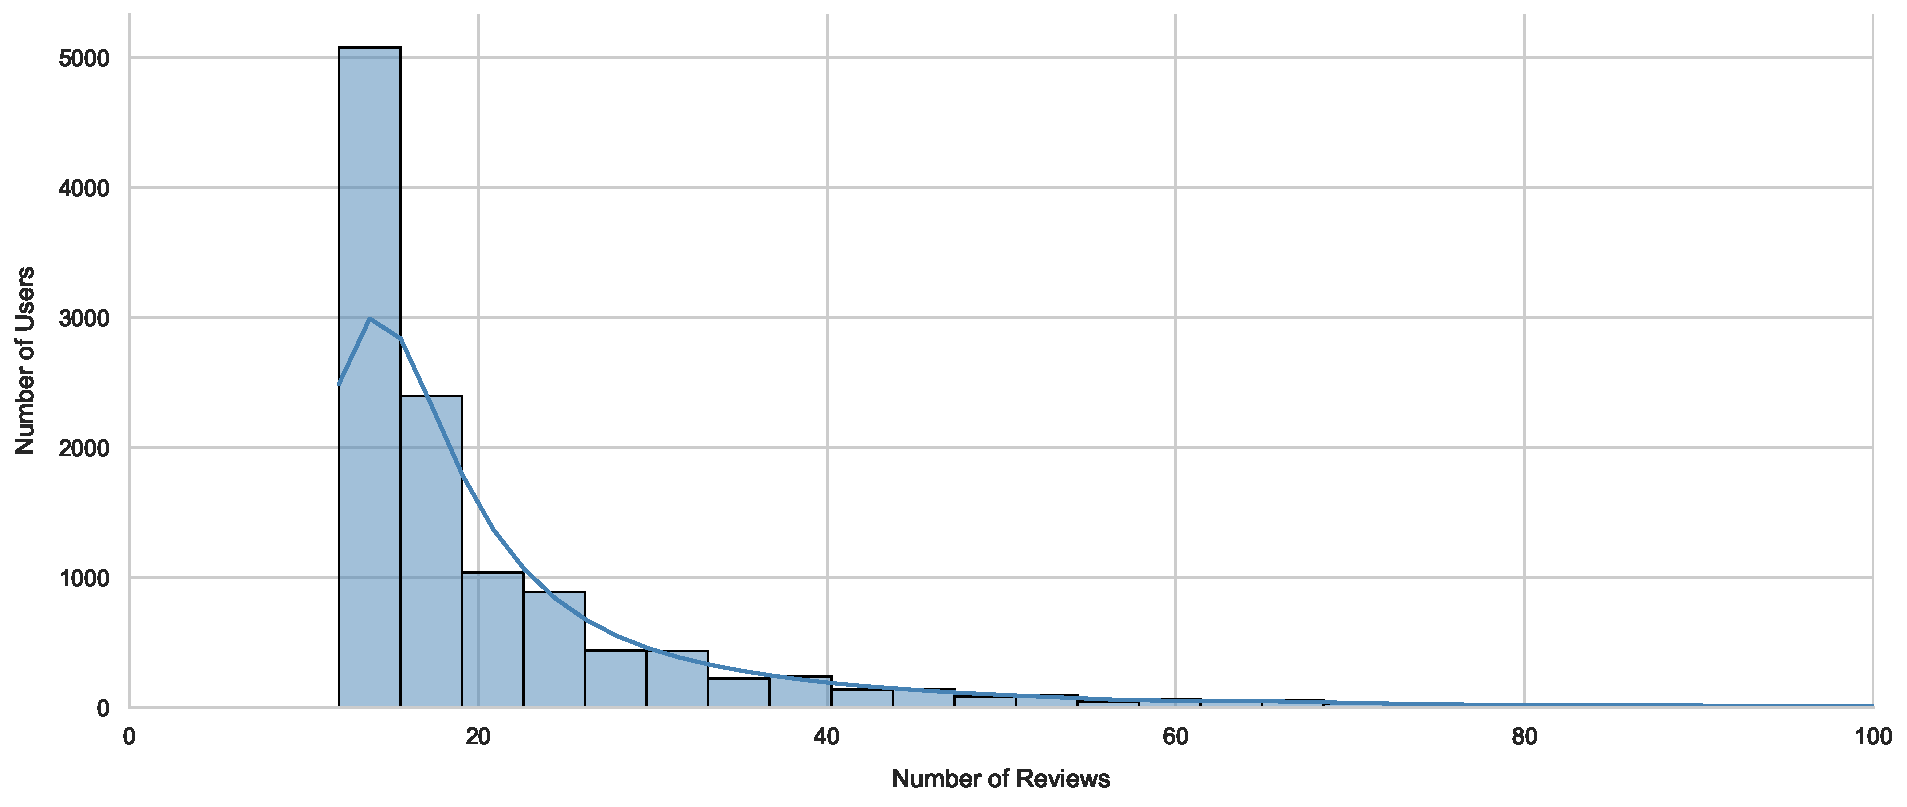
\includegraphics[width=0.9\textwidth]{Figures/reviews_per_user_distribution.pdf} % Adjust the width as needed
  \caption{Distribution of Reviews per Reviewer.}
  \label{fig:user review distribution}
\end{figure}

Additionally, a temporal analysis, shown in Figure \ref{fig:reviews per year}, illustrates an increasing trend in the number of reviews over time which illustrates an increasing trend in user engagement. Specifically, the line chart in Figure \ref{fig:reviews per year} displays the trend in the number of reviews per year from 1998 to 2018. It is clear that the number of reviews has experienced exponential growth over the years. The review count remains relatively low until around 2010, after which there is a sharp increase, indicating a surge in user engagement on the platform. This trend of exponential growth is a common characteristic of user-generated content on digital platforms, reflecting the rapid adoption and increasing popularity of online shopping and product reviews \cite{alzoubi2022effect}. In 2017, the review count reaches its peak at 57,934, demonstrating the high level of user engagement during this period. However, there is a noticeable dip in the number of reviews in 2018, with the count dropping to 12,042. This decline is not indicative of a decrease in user engagement but it is likely due to the dataset only containing reviews up until February 2018. Therefore, the data for 2018 is not complete, which explains the sudden drop.

\begin{figure}[ht]
  \centering
  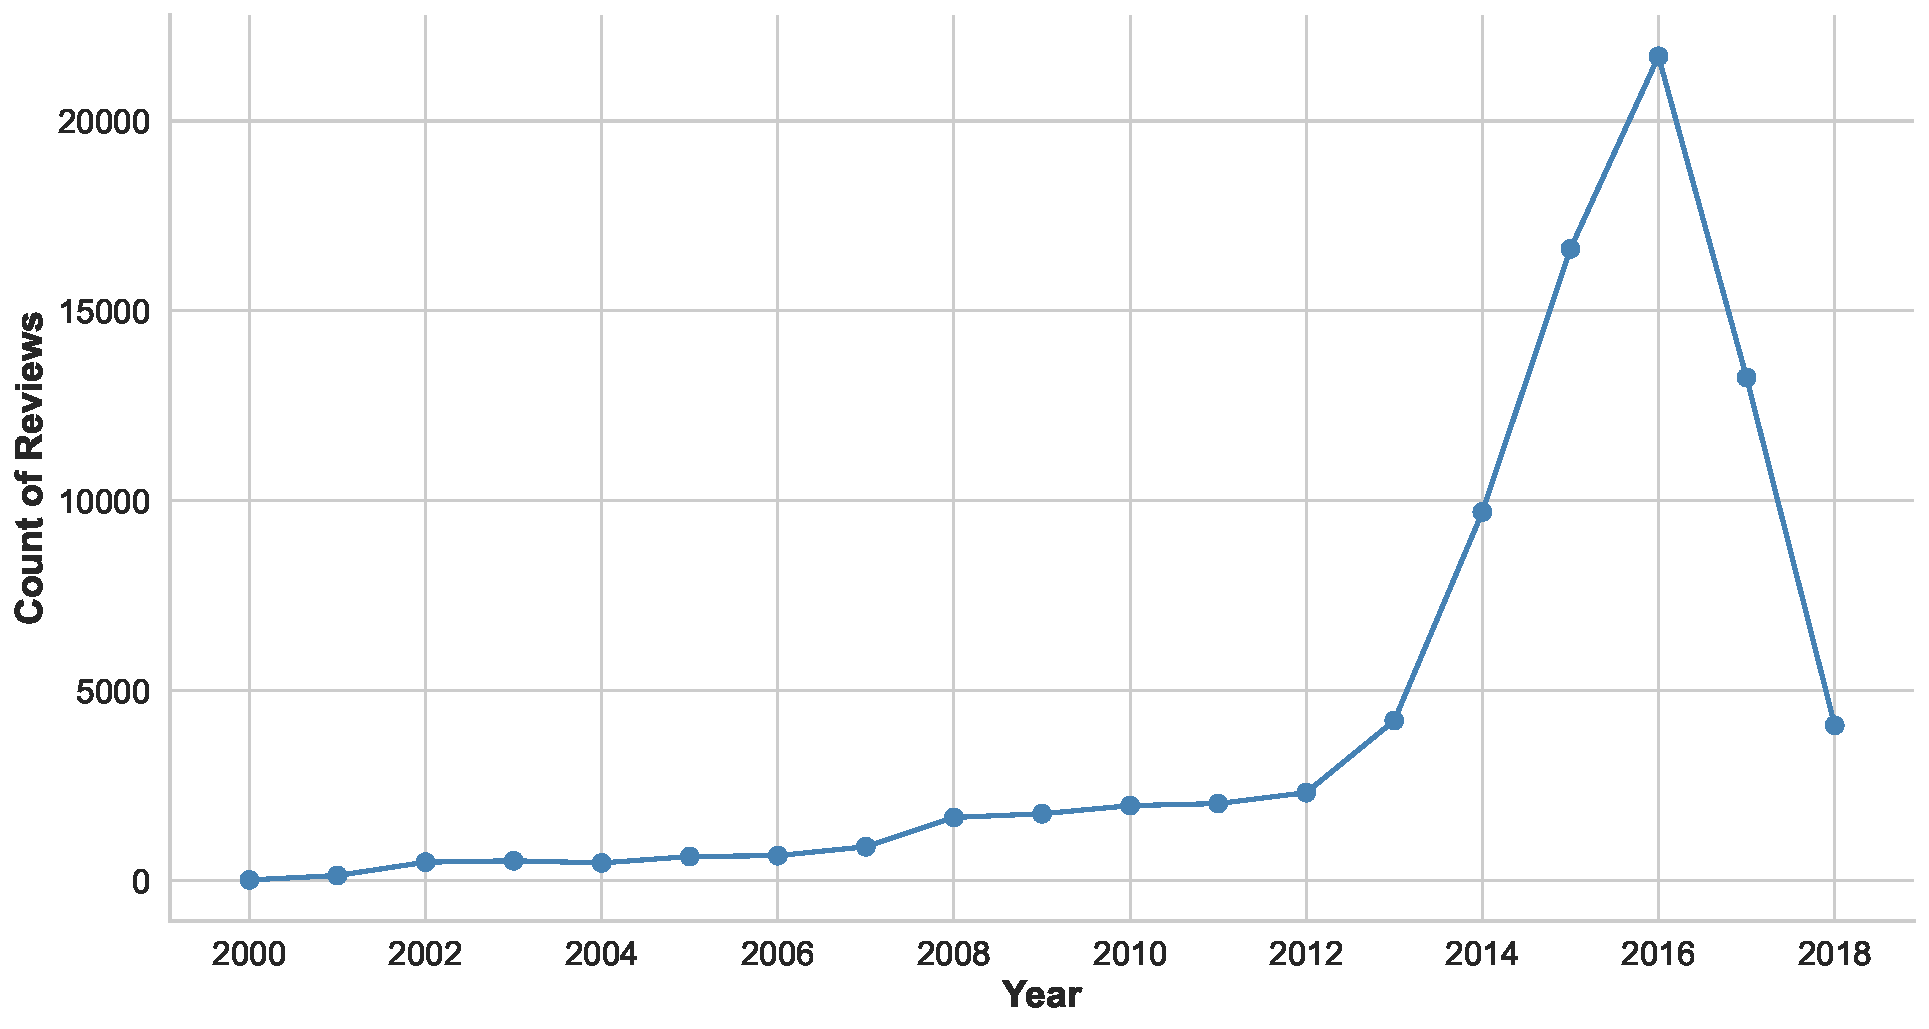
\includegraphics[width=0.9\textwidth]{Figures/reviews_per_year.pdf} % Adjust the width as needed
  \caption{Number of Reviews per Year.}
  \label{fig:reviews per year}
\end{figure}

These figures have provided valuable insights into the general user engagement, and in extension the temporal dynamics of user engagement in terms of review contribution on Amazon's e-commerce platform. Although the temporal aspect is not considered in this thesis, it is worthwhile showing to provide context on the dataset chosen. 

\subsection{Products}
\label{subsec:3 Products}

Similar to Figure \ref{fig:user review distribution}, we can look at the number of reviews per product. Analysing this is essential for shedding light on the dynamics and characteristics of the dataset that extend beyond individual user behaviors. Figure \ref{fig:product review distribution} illustrates the number of reviews per product. From the Figure, it is evident that a significant number of products have received fewer than 40 reviews, with a peak frequency observed for products with around 12 to 20 reviews. This suggests that while some products receive a high volume of reviews, the majority tend to have a relatively lower count.

Importantly, the figure aligns with our data subsetting process of ensuring that each product has at least 13 reviews. Again, this was done to alleviate the cold start problem, ensuring that there is sufficient interaction data for each product to generate reliable recommendations. Similar to Figure \ref{fig:user review distribution}, this product distribution is right skewed and the median number of reviews per product is 24.5. 

\begin{figure}[h]
  \centering
  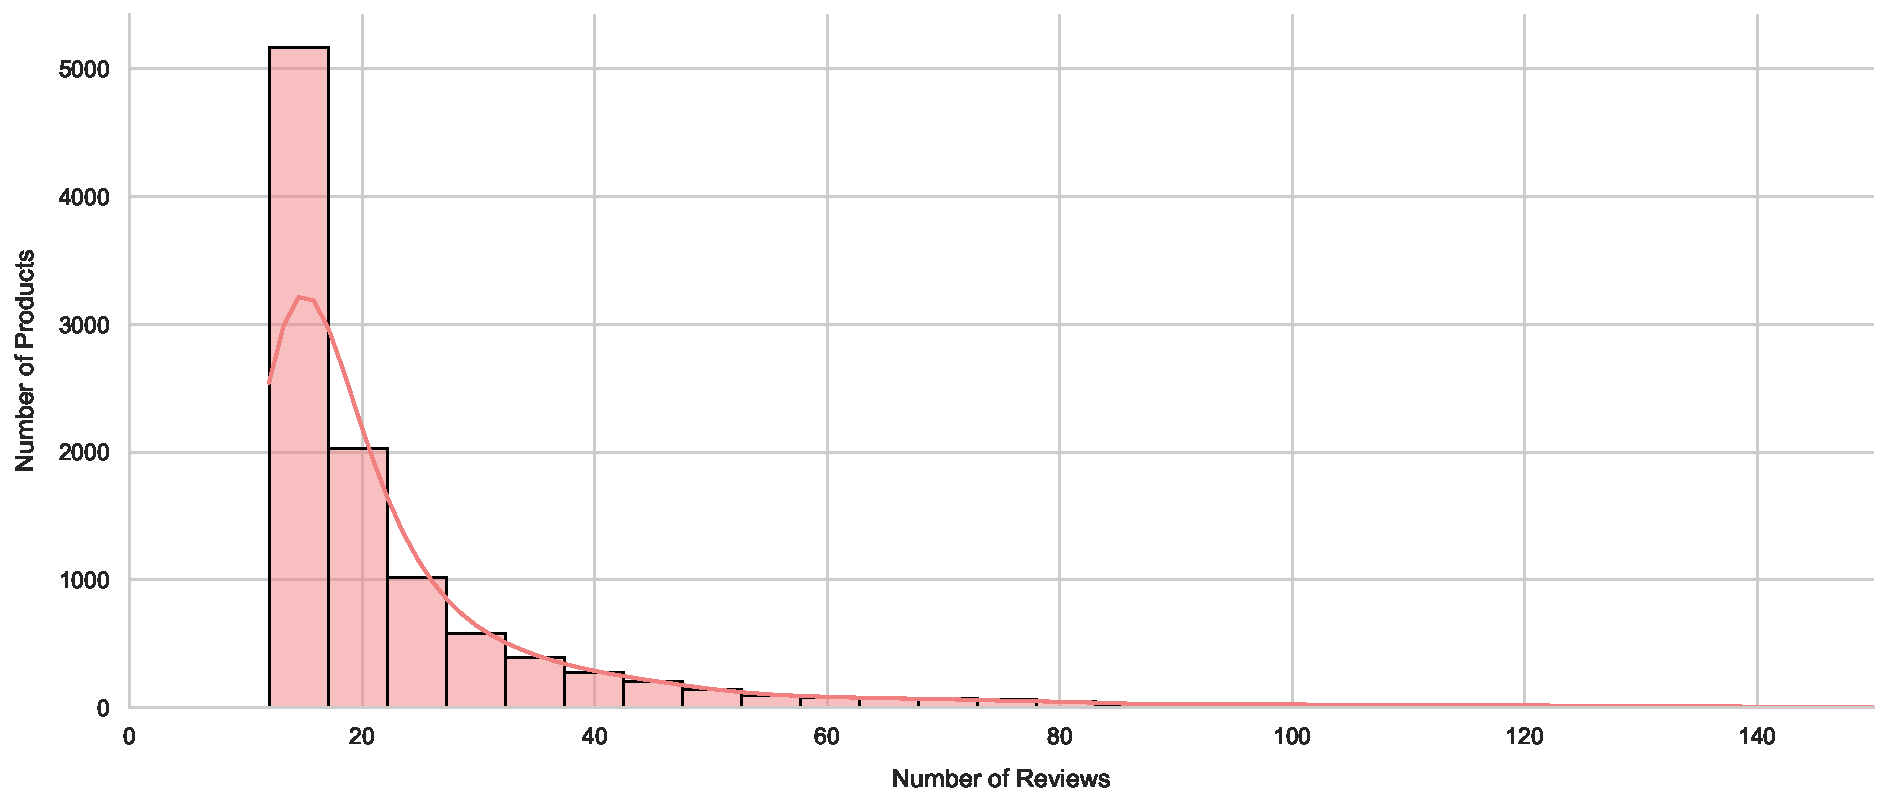
\includegraphics[width=0.9\textwidth]{Figures/reviews_per_product_distribution.pdf} % Adjust the width as needed
  \caption{Distribution of Reviews per Product.}
  \label{fig:product review distribution}
\end{figure}


\subsection{Ratings}
\label{subsec:3 Ratings}

We can also generate an overall picture of the dataset by looking at the distribution of ratings - allowing us to discern the user's general perception toward the products in our dataset. Figure \ref{fig:ratings distribution}, illustrates the the spread and central tendency of ratings. As mentioned in Section \ref{subsec:Amazon Review Dataset}, the rating scale is 1 to 5 for this Amazon Product Reviews dataset. From the Figure, it is clear that the majority of users have given a rating of 5, with the count exceeding 160,000 reviews. This suggests a high level of customer satisfaction, indicating that most users had positive experiences with the products they reviewed. On the other end of the spectrum, very few users have given ratings of 1 and 2, with counts of 7,606 and 8,465 respectively. This suggests that negative experiences are relatively rare among the users. Nevertheless, this scarcity could be indicative of two potential scenarios: either negative encounters are genuinely uncommon, or users may not be as prompt to express dissatisfaction compared to their enthusiasm in sharing positive experiences (\cite{chen2015augmenting};\cite{skalicky2015statistical})

\begin{figure}[h]
  \centering
  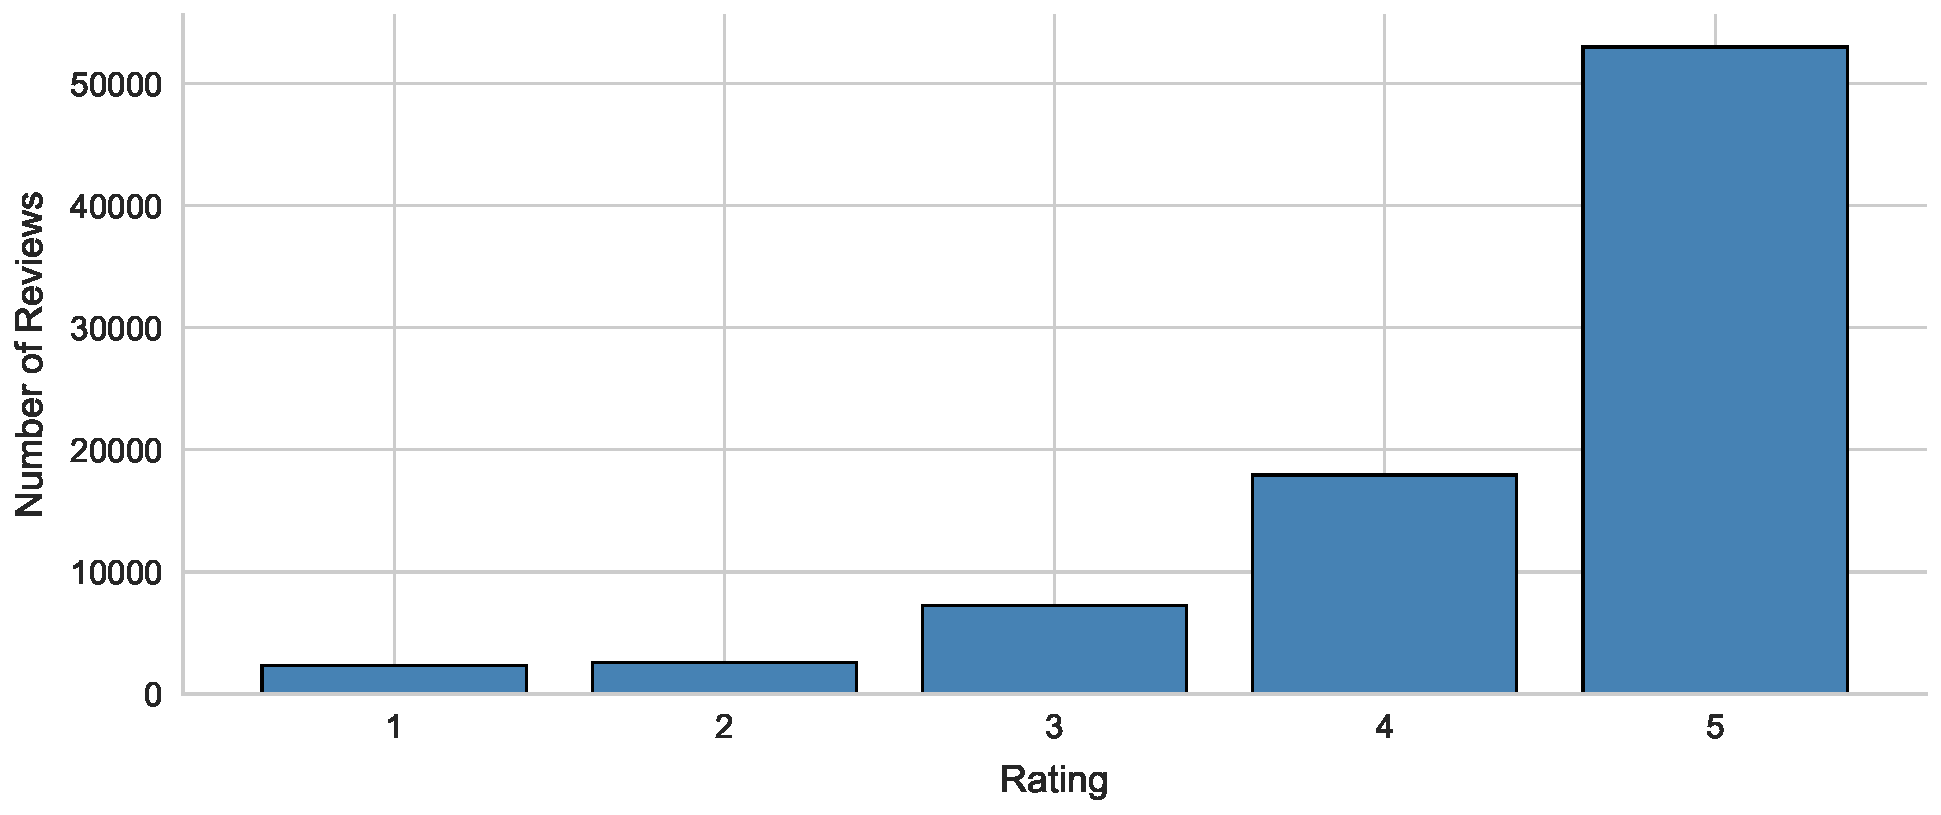
\includegraphics[width=0.9\textwidth]{Figures/rating_distribution.pdf} % Adjust the width as needed
  \caption{Distribution of Ratings from Users.}
  \label{fig:ratings distribution}
\end{figure}

Ultimately, understanding the distribution of user ratings is crucial for building and optimising our recommender system as it plays a large role in informing us of the potential user bias. We complement this Figure by looking at the the summary statistics in Table \ref{tab:rating summary}, for the ratings attribute which again reiterates how a large portion of the ratings are highly rated (5). Furthermore, the mean rating of 4.4 highlights the positive trend in the user feedback. Sentiment analysis scores could perhaps adjust for this bias, as they provide a more nuanced understanding of user preferences and opinions, which can potentially enhance the recommenders  ability to better capture the user's preferences and satisfaction with products and ultimately provide more accurate and relevant recommendations \cite{dang2021approach}.

\begin{table}[ht]
  \centering
  \begin{tabular}{l c}
      \hline
      \textbf{Statistic} & \textbf{Value} \\
      \hline
      Count & 294,255 \\
      Mean & 4.41 \\
      Standard Deviation & 0.98 \\
      Minimum & 1 \\
      25\% Percentile & 4 \\
      50\% Percentile & 5 \\
      75\% Percentile & 5 \\
      Maximum & 5 \\
      \hline
  \end{tabular}
  \caption{Summary Statistics of Ratings}
  \label{tab:rating summary}
\end{table}

\subsection{Review Text and Sentiments}
\label{subsec:3 Review Text}

Regarding the review, we have spent a considerable amount of time cleaning and preprocessing the this feature. We can now explore it, both from a lens of the textual content and the sentiments - the goal being to visualise and iedentify any patterns within the user reviews or sentiments. 

On average, we found that there are 116 words in each review. To supplement this, we visualise the distribution of the word count in Figure \ref{fig:distribution of word count}. From the Figure, it is clear that a majority of the reviews are relatively short, with most falling under 200 words - with large number of reviews containing somewhere in the region of 100 words. This suggests that users typically prefer to leave concise feedback on products. Since we are looking at incorporating these reviews into NCF models, this could have several implications. Given that shorter reviews are more frequent, they might have a more significant impact on the prediction outcomes. However, shorter reviews might not always provide comprehensive insights into a user’s preferences or experiences, as they might lack detailed descriptions or explanations. On the other hand, longer reviews, although less frequent, might offer more detailed insights into a user’s preferences, potentially enhancing the accuracy of the recommendations. However, they might also introduce noise into the model due to the increased likelihood of off-topic content or unnecessary details. A potential outcome of this is that the model might be biased towards shorter reviews, as they are more frequent \cite{srifi2020recommender}. This shall be explored further in the Chapter \ref{Chapter5} - the results.

\begin{figure}[h]
  \centering
  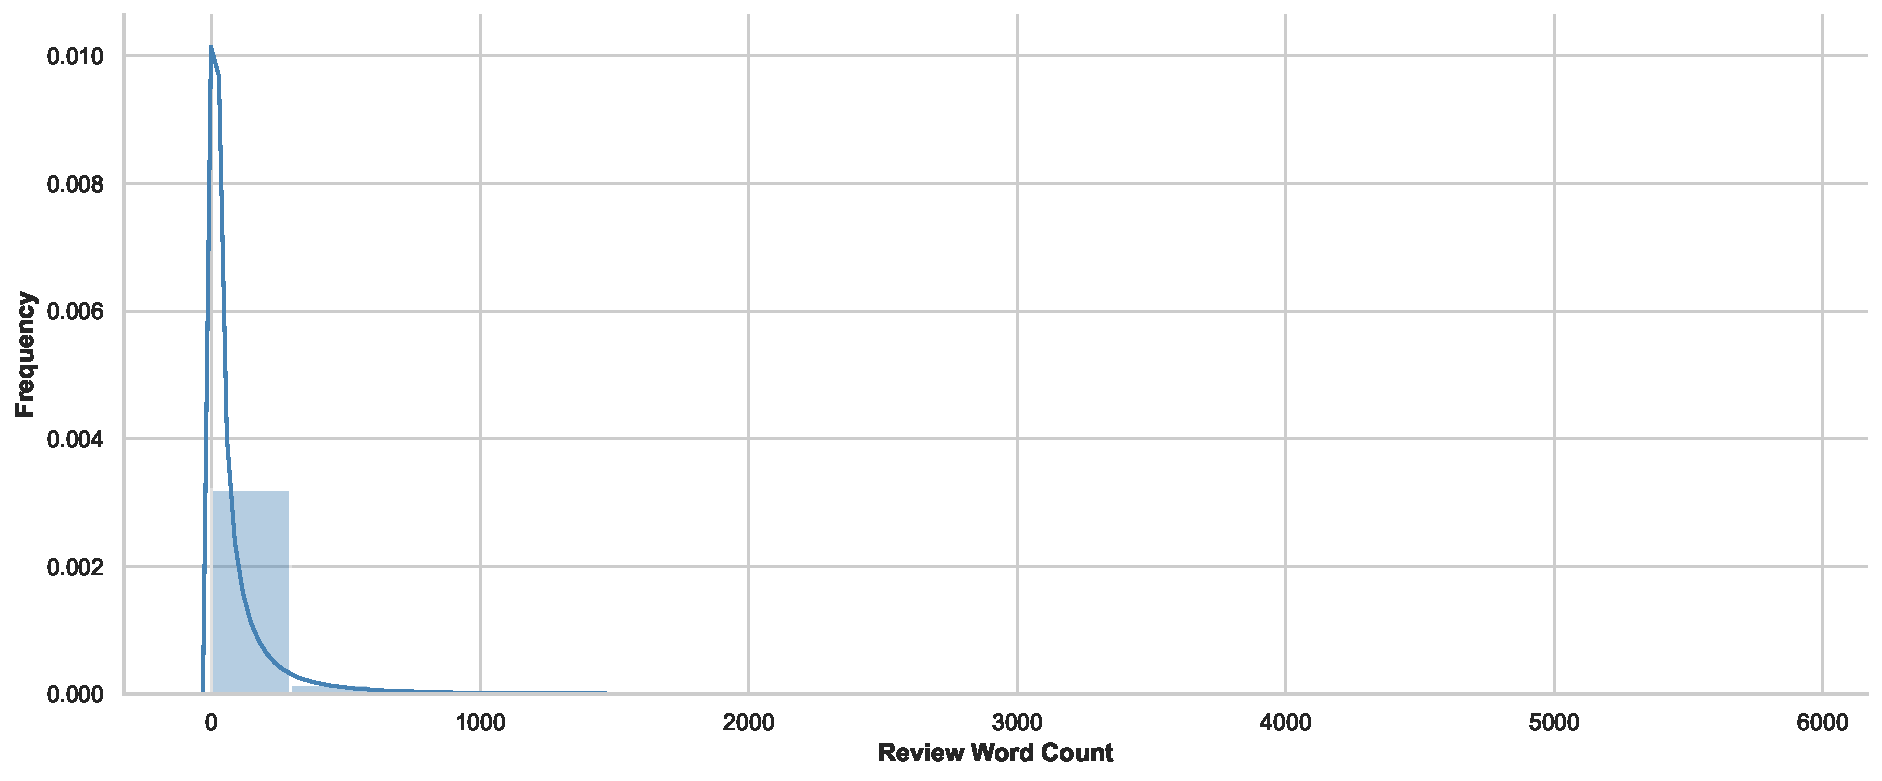
\includegraphics[width=0.9\textwidth]{Figures/distribution_of_review_word_count.pdf} % Adjust the width as needed
  \caption{Distribution of Review Word Count.}
  \label{fig:distribution of word count}
\end{figure}

Using the review text we can also explore the prevalence of specific phrases or consecutive words, commonly known as $n$-grams, where $n$ is the number of words \cite{mcauley2013hidden}. In Figure \ref{fig:n-grams}, we specifically examine the top 10 frequently occurring consecutive tri-grams (Figure \ref{fig:trigrams}) and four-grams (Figure \ref{fig:four-grams}). This analysis provides insights into the distinctive linguistic structures that frequently appear in the reviews, improving our understanding of the language dynamics within the dataset.

\begin{figure}[h]
  \centering
  \begin{subfigure}{0.48\textwidth}
      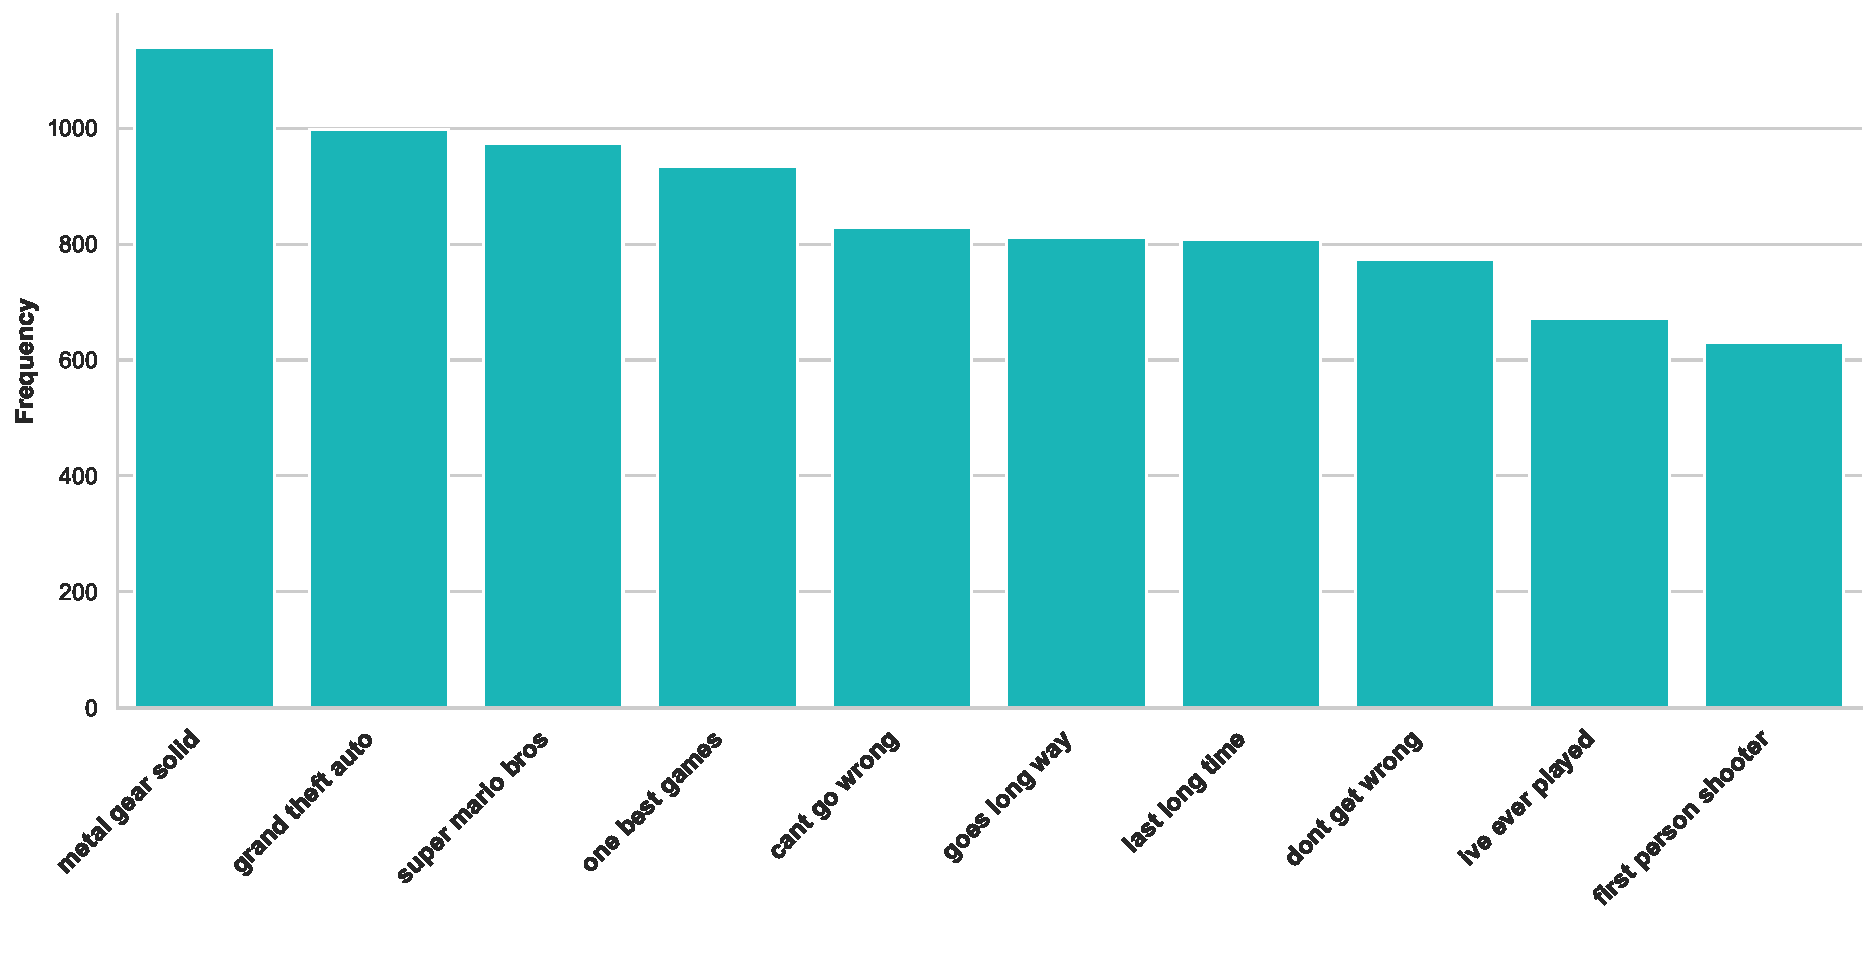
\includegraphics[width=\textwidth]{Figures/trigrams.pdf} % Adjust the file path and width as needed
      \caption{Tri-gram}
      \label{fig:tri-grams}
  \end{subfigure}
  \hfill
  \begin{subfigure}{0.48\textwidth}
      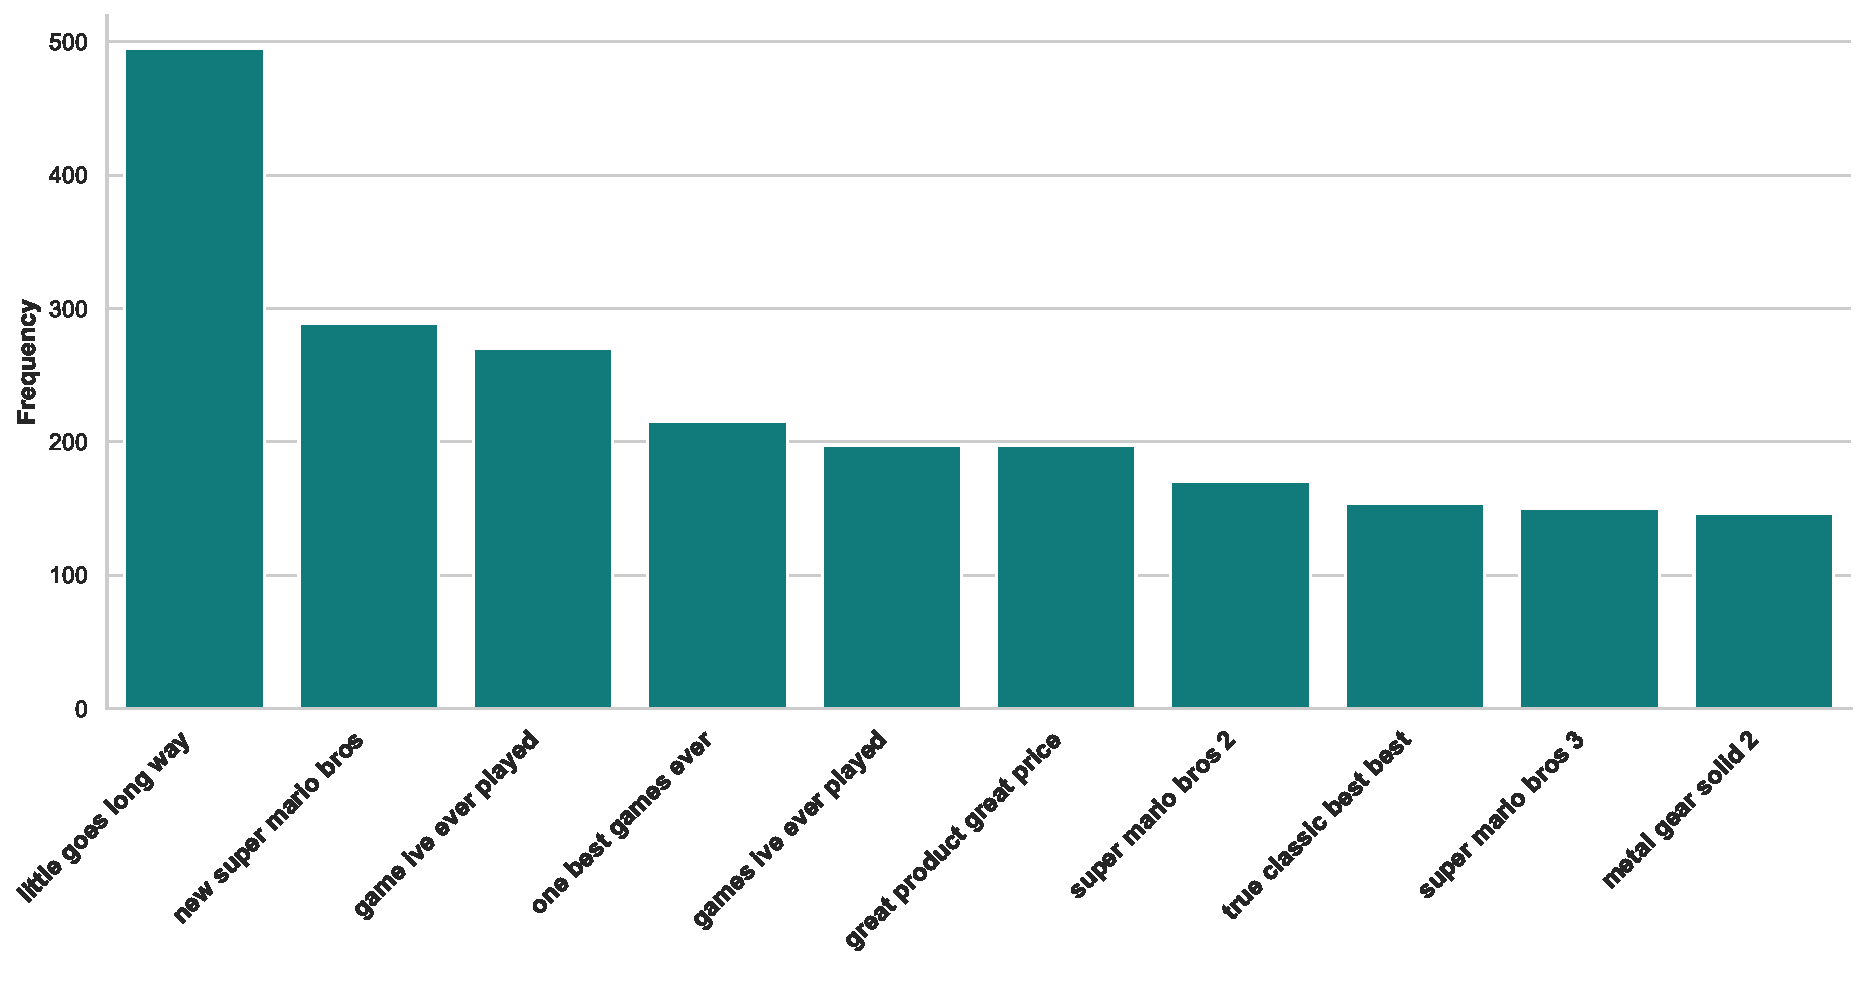
\includegraphics[width=\textwidth]{Figures/fourgrams.pdf} % Adjust the file path and width as needed
      \caption{Four-gram}
      \label{fig:four-grams}
  \end{subfigure}
  \caption{Top 10 N-grams in Review Text from Users}
  \label{fig:n-grams}
\end{figure}

From the Figure \ref{fig:n-grams}, it is clear that phrases like “metal gear solid”, “grand theft auto”, and “super mario bros” are among the most frequent tri-grams. These tri-grams appear to be related to popular video game titles, suggesting that our dataset includes a significant amount of reviews for these games or rather, users frequently mention these games in their reviews. This could be indicative of the popularity of these games among users. Other tri-grams like “one best games”, “can’t go wrong”, and “goes long way” could be common phrases users employ to express their positive experiences or high regard for a product.  We find similar results when we look at the four-grams (Figure \ref{fig:four-grams}) where some of the phrases are  “little goes long way”, “now super mario bros”, and “one best games ever” are among the most frequently used. 

These $N$-grams are useful in text analysis as they provide context that individual words might not. By considering sequences of words (like tri-grams and four-grams), we can capture more meaningful phrases that often occur in our text data. This can help in understanding common themes or topics in our reviews \cite{collins2019document}. Furthermore, in the context of our recommender system, these $n$-grams can provide valuable insights into the aspects that users frequently discuss or value in products \cite{srifi2020recommender}. However, it’s important to note that while $n$-grams can capture local context (i.e., within the $n$-gram), they might not capture the overall sentiment of a review if it’s expressed through complex or long-range dependencies between words. Techniques like sentiment analysis, which we employed, are more effective in capturing the overall sentiment of a review, as they consider the entire review text \cite{collins2019document}.

To that end, we can also explore the distribution of the sentiment scores from from each of the three sentiment analysis lexicon-based methods in Figure \ref{fig:comparison_sentiments}. From Figure \ref{fig:comparison_sentiments}, it is clear that the distribution of sentiment scores from AFINN (Figure \ref{fig:afinn sentiment distribution}) and BING (Figure \ref{fig:bing sentiment distribution}) are similar, while the distribution of sentiment scores from VADER (Figure \ref{fig:vader sentiment distribution}) is distinct. For AFINN and BING, their distributions are uni-modal and skewed to the right, with most sentiment scores concentrated around 0. This suggests that these sentiment analysis techniques tends to classify a significant portion of the reviews as neutral. In contrast to Figures \ref{fig:bing sentiment distribution} and \ref{fig:afinn sentiment distribution}, the sentiment score distribution for VADER (Figure \ref{fig:vader sentiment distribution}) illustrates sentiment scores not uniformly distributed. Most of the sentiment scores are clustered around 0 and 1, indicating that most reviews are either neutral or positive. There is a significant spike in frequency close to the 1.00 score, suggesting a high volume of very positive sentiments in the reviews. Given that we have spikes at 0, 1 scores, as well as some reviews classified negatively (as shown in Figure \ref{fig:vader sentiment distribution}), we find that the distribution of VADER sentiments illustrates that this technique is capturing both the positive, neutral, and negative sentiments in our review data, albeit with a higher frequency of positive sentiments. We expect this behaviour since the distribution of ratings (as shown in Figure \ref{fig:ratings distribution}) is heavily skewed towards the higher ratings.

As we mentioned in Section \ref{subsec:3 Sentiment Analysis} we opted for VADER as it held the strongest correlation with the user ratings. This decision seems well-supported as VADER, unlike AFINN and BING, captures a wider range of sentiments (as shown from Figure \ref{fig:vader sentiment distribution}), which could lead to a more nuanced understanding of user opinions. This can be particularly useful for our recommender system as it can help in capturing more detailed user preferences, potentially enhancing the accuracy of our recommendations \cite{dang2021approach}. 


\begin{figure}[h]
  \centering
  \begin{subfigure}{0.32\textwidth} % Adjust the width based on the number of figures
      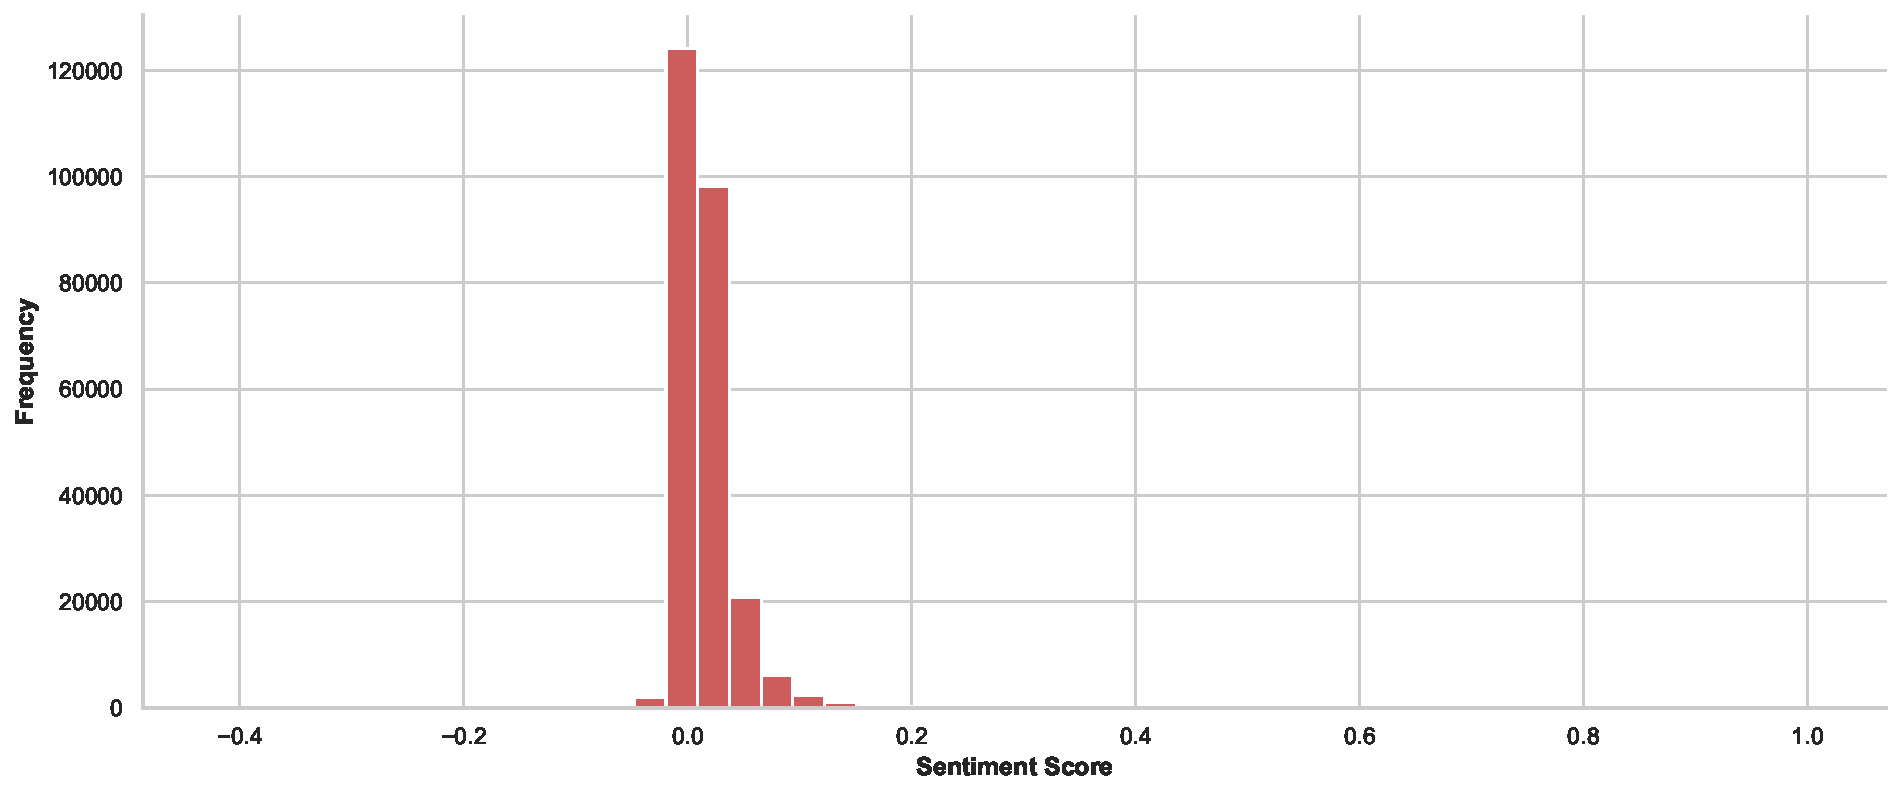
\includegraphics[width=\textwidth]{Figures/distribution_afinn.pdf} % Adjust the file path and width as needed
      \caption{AFINN}
      \label{fig:afinn sentiment distribution}
  \end{subfigure}
  \hfill
  \begin{subfigure}{0.32\textwidth} % Adjust the width based on the number of figures
      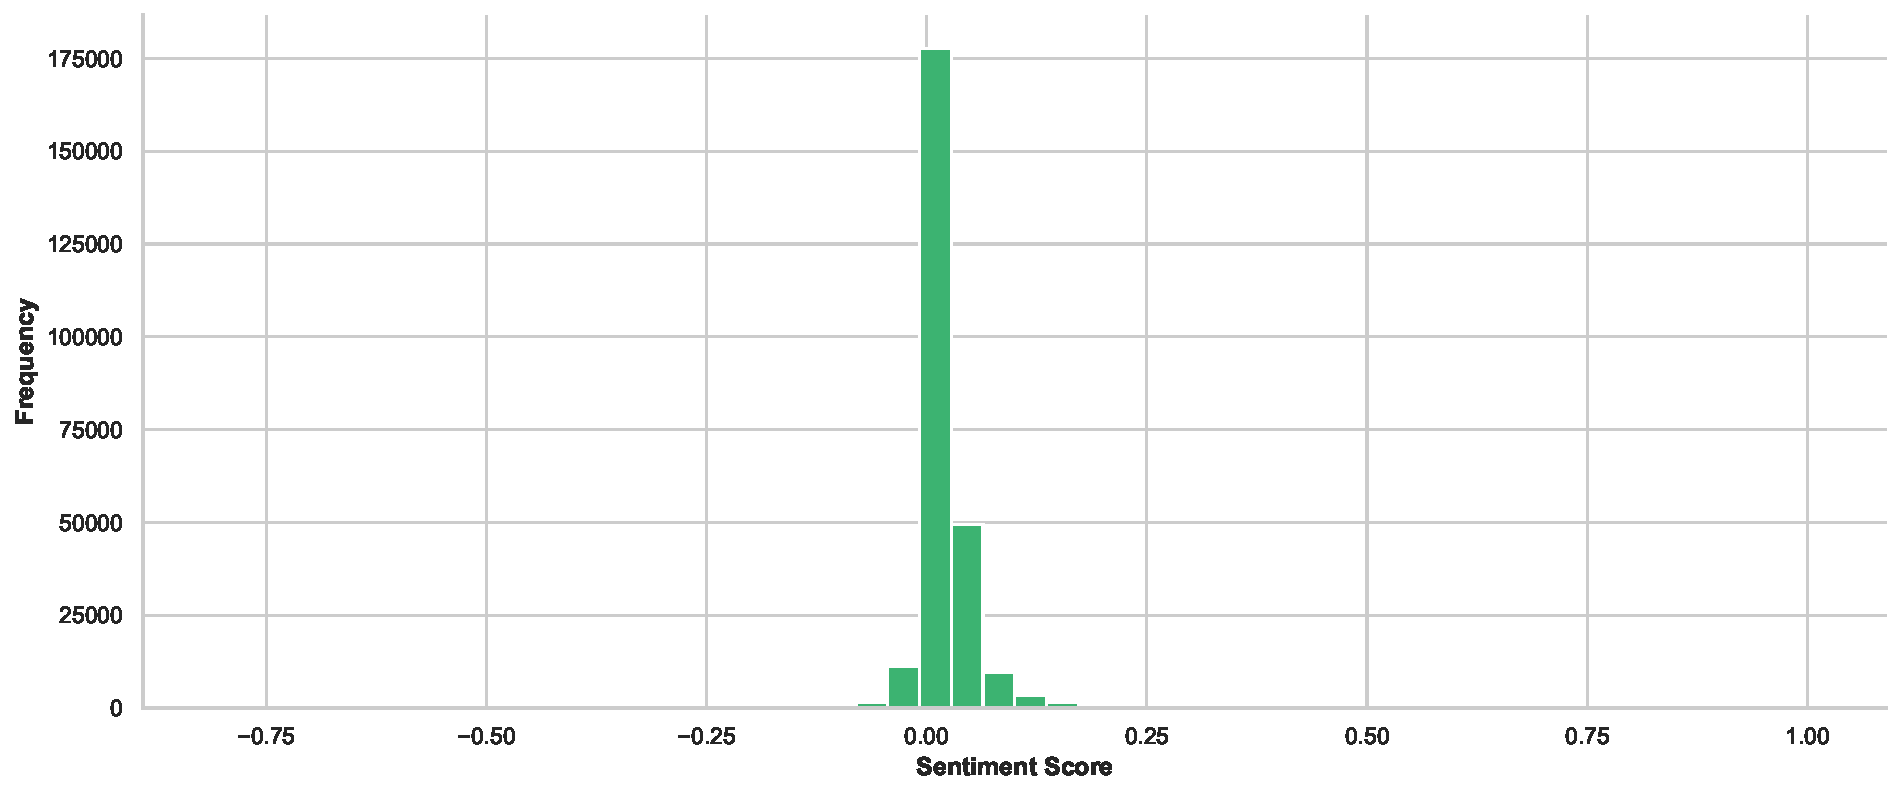
\includegraphics[width=\textwidth]{Figures/distribution_bing.pdf} % Add the path to the third figure
      \caption{BING} % Add a caption for the third figure
      \label{fig:bing sentiment distribution} % Add a label for the third figure
  \end{subfigure}
  \hfill
  \begin{subfigure}{0.32\textwidth} % Adjust the width based on the number of figures
      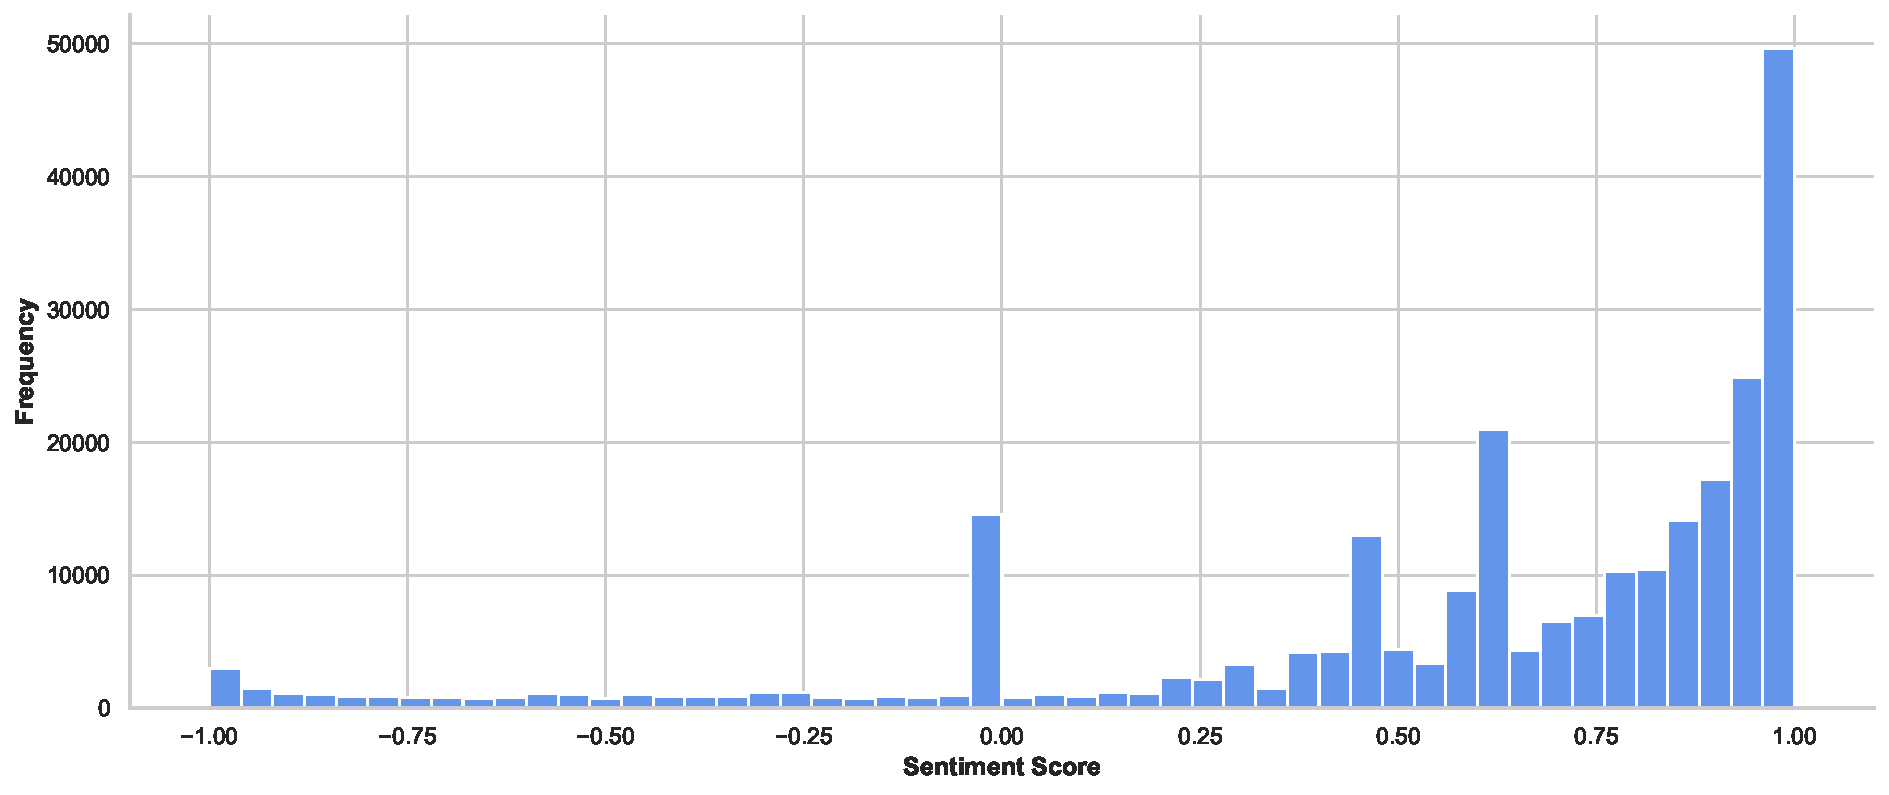
\includegraphics[width=\textwidth]{Figures/distribution_vader.pdf} % Adjust the file path and width as needed
      \caption{VADER}
      \label{fig:vader sentiment distribution}
  \end{subfigure}
  \caption{Distribution of Sentiment Scores for AFINN, BING and VADER algorithms.} % Update the caption accordingly
  \label{fig:comparison_sentiments}
\end{figure}

In Figures \ref{fig:top 10 products sentiments} and \ref{fig:bottom 10 products sentiments}, we identify the the top 10 products and bottom 10 products based on their average sentiment scores. We see that the top products have very similar mean sentiment scores. In contrast, there is a clearer difference between the bottom 10 products. Additionally, Tables \ref{tab:top 10 products statistics} and \ref{tab:bottom 10 products statistics} illustrates that the ratings for the top 10 and bottom 10 products (by sentiment) line up quite well. This is indicative of a consistent correlation between product (VADER) sentiment and user ratings, suggesting that products with higher sentiment scores tend to receive more positive ratings, while those with lower sentiment scores align with lower ratings. 

\begin{figure}[h]
  \centering
  \begin{subfigure}{0.48\textwidth}
      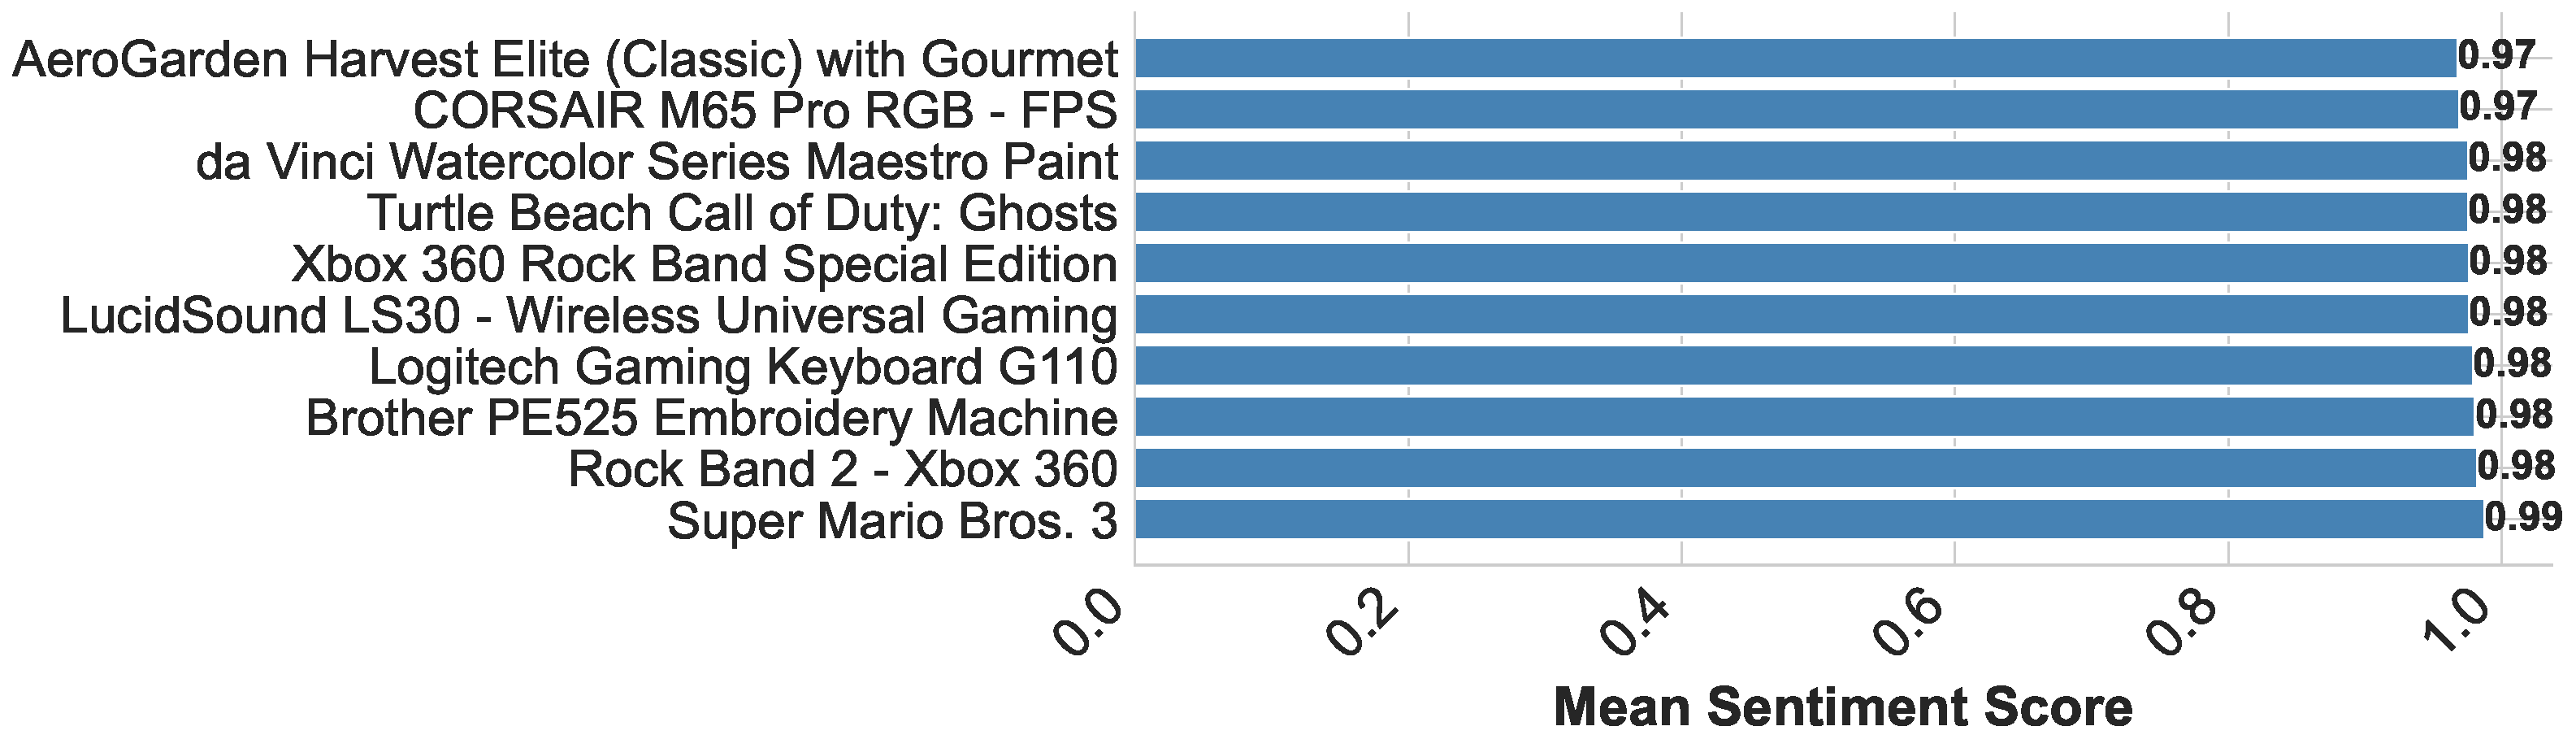
\includegraphics[width=\textwidth]{Figures/Top_10_Products_Sentiments.pdf} % Adjust the file path and width as needed
      \caption{Top 10 Products Sentiments}
      \label{fig:top 10 products sentiments}
  \end{subfigure}
  \hfill
  \begin{subfigure}{0.48\textwidth}
      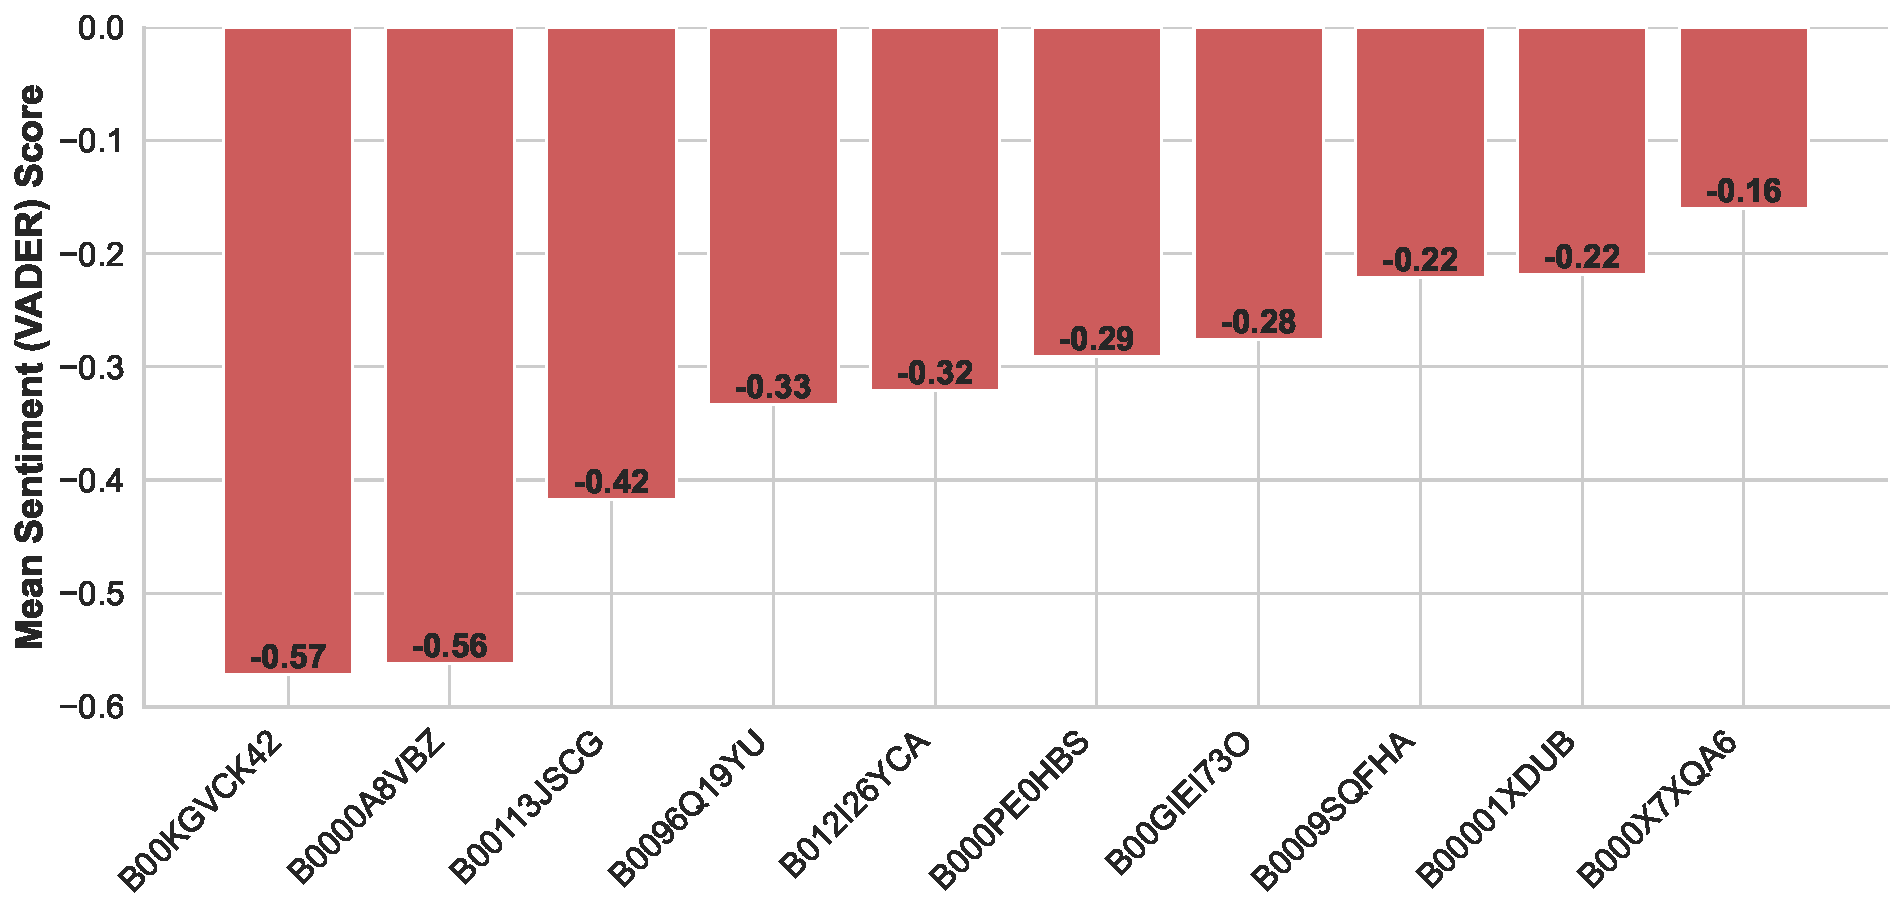
\includegraphics[width=\textwidth]{Figures/Bottom_10_Products_Sentiments.pdf} % Adjust the file path and width as needed
      \caption{Bottom 10 Products Sentiments}
      \label{fig:bottom 10 products sentiments}
  \end{subfigure}
  \caption{Comparison of Sentiments for Top and Bottom 10 Products}
  \label{fig:comparison_sentiments_top_10s}
\end{figure}

\begin{table}[h]
  \centering
  \begin{tabular}{cccc}
      \hline
      \textbf{ASIN} & \textbf{Count of Reviews} & \textbf{Mean Rating} & \textbf{Mean Sentiment} \\
      \hline
      B00RBQV2XK & 13 & 4.538 & 0.981 \\
      B000TT4GBG & 16 & 4.312 & 0.977 \\
      B000WINB56 & 17 & 4.235 & 0.977 \\
      B00LYYMXF6 & 14 & 5     & 0.977 \\
      B00BB5HU6K & 13 & 4.462 & 0.976 \\
      B00D96BNGM & 19 & 4.526 & 0.976 \\
      B0171155ZU & 13 & 4.923 & 0.975 \\
      B00KAYDYE0 & 14 & 4.857 & 0.974 \\
      B0007TFCFW & 13 & 4.923 & 0.974 \\
      B00004U9MS & 12 & 3.917 & 0.974 \\
      \hline
  \end{tabular}
  \caption{Details about the Top 10 Products by Average Sentiment}
  \label{tab:top 10 products statistics}
\end{table}


\begin{table}[h]
  \centering
  \begin{tabular}{cccc}
      \hline
      \textbf{ASIN} & \textbf{Count of Reviews} & \textbf{Mean Rating} & \textbf{Mean Sentiment} \\
      \hline
      B00KGVCJX4 & 16 & 3.875 & -0.312 \\
      B00004SPW9 & 13 & 3.9230 & -0.323 \\
      B00005JO16 & 13 & 3.461 & -0.325 \\
      B000059HCH & 14 & 3.643 & -0.341 \\
      B000VKL6Z2 & 16 & 3.938 & -0.371 \\
      B0011G6FDI & 15 & 3.467 & -0.397 \\
      B000XJO78Y & 13 & 2.769 & -0.462 \\
      B0096Q19YU & 18 & 3.444 & -0.479 \\
      B00KGVCK42 & 16 & 4.375 & -0.492 \\
      B00008DDVU & 12 & 3.833 & -0.670 \\
      \hline
  \end{tabular}
  \caption{Details about the Bottom 10 Products by Average Sentiment}
  \label{tab:bottom 10 products statistics}
\end{table}

The products with high sentiments (see Figure \ref{fig:top 10 products sentiments}) have received high positive feedback from users and furthermore, from Table \ref{tab:top 10 products statistics} we see that these products also have at least a mean rating of 4 (and more often than not closer to 5). This further reinforces the positive sentiment towards these products, indicating that they are well-received by users in terms of both ratings and review sentiments. We can say the same for the for bottom 10 products shown in Figure \ref{fig:bottom 10 products sentiments}  and Table \ref{fig:bottom 10 products sentiments} - these low mean sentiments achieved by these products reviews are also reflected in their mean ratings being mostly below 4.

To end off this visual analysis, Figure \ref{fig:correlation heat map sentiments} is a correlation heat map displaying the relationship between the various sentiment scores generated from AFINN, BING and VADER as well as the ratings and review word count. The goal here is to illustrate  whether there is a correlation between any of these sentiment scores with the ratings, and whether review length has a correlation with sentiments or ratings. From Figure \ref{fig:correlation heat map sentiments}, it is clear that VADER has the highest correlation with rating (0.32), suggesting a moderate positive relationship. This indicates that as the VADER sentiment score increases, the rating tends to increase as well. This is an important observation and was pivotal to our decision to use VADER as the sentiment analysis method of choice to generate sentiments to be used in our model Specifically, AFINN and BING have lower correlations with rating (0.09 and 0.13 respectively), indicating weaker relationships with the rating.  Word count has a negative correlation with rating (-0.13), suggesting that longer reviews tend to have lower ratings - albeit the correlation is very weak. However, it has positive correlations with all three sentiment analysis techniques, with the highest being with AFINN (0.59). However, this is also an expected result, as AFINN (and BING) assign sentiment scores to each word in a review, and the cumulative score is influenced by the number of words \cite{haque2018sentiment}. Consequently, reviews with more words have a greater chance of containing positive words, resulting in higher sentiment scores. 

Ultimately, this section has provided us with a holistic understanding of the dataset's inherent structures and offers context-rich insights that will guide subsequent modelling, interpretation and discussions. However, before we detail the next steps, it is important to establish what data is used to train our models and what data is used to validate our models - this is studied in the next section. 

\begin{figure}[h]
  \centering
  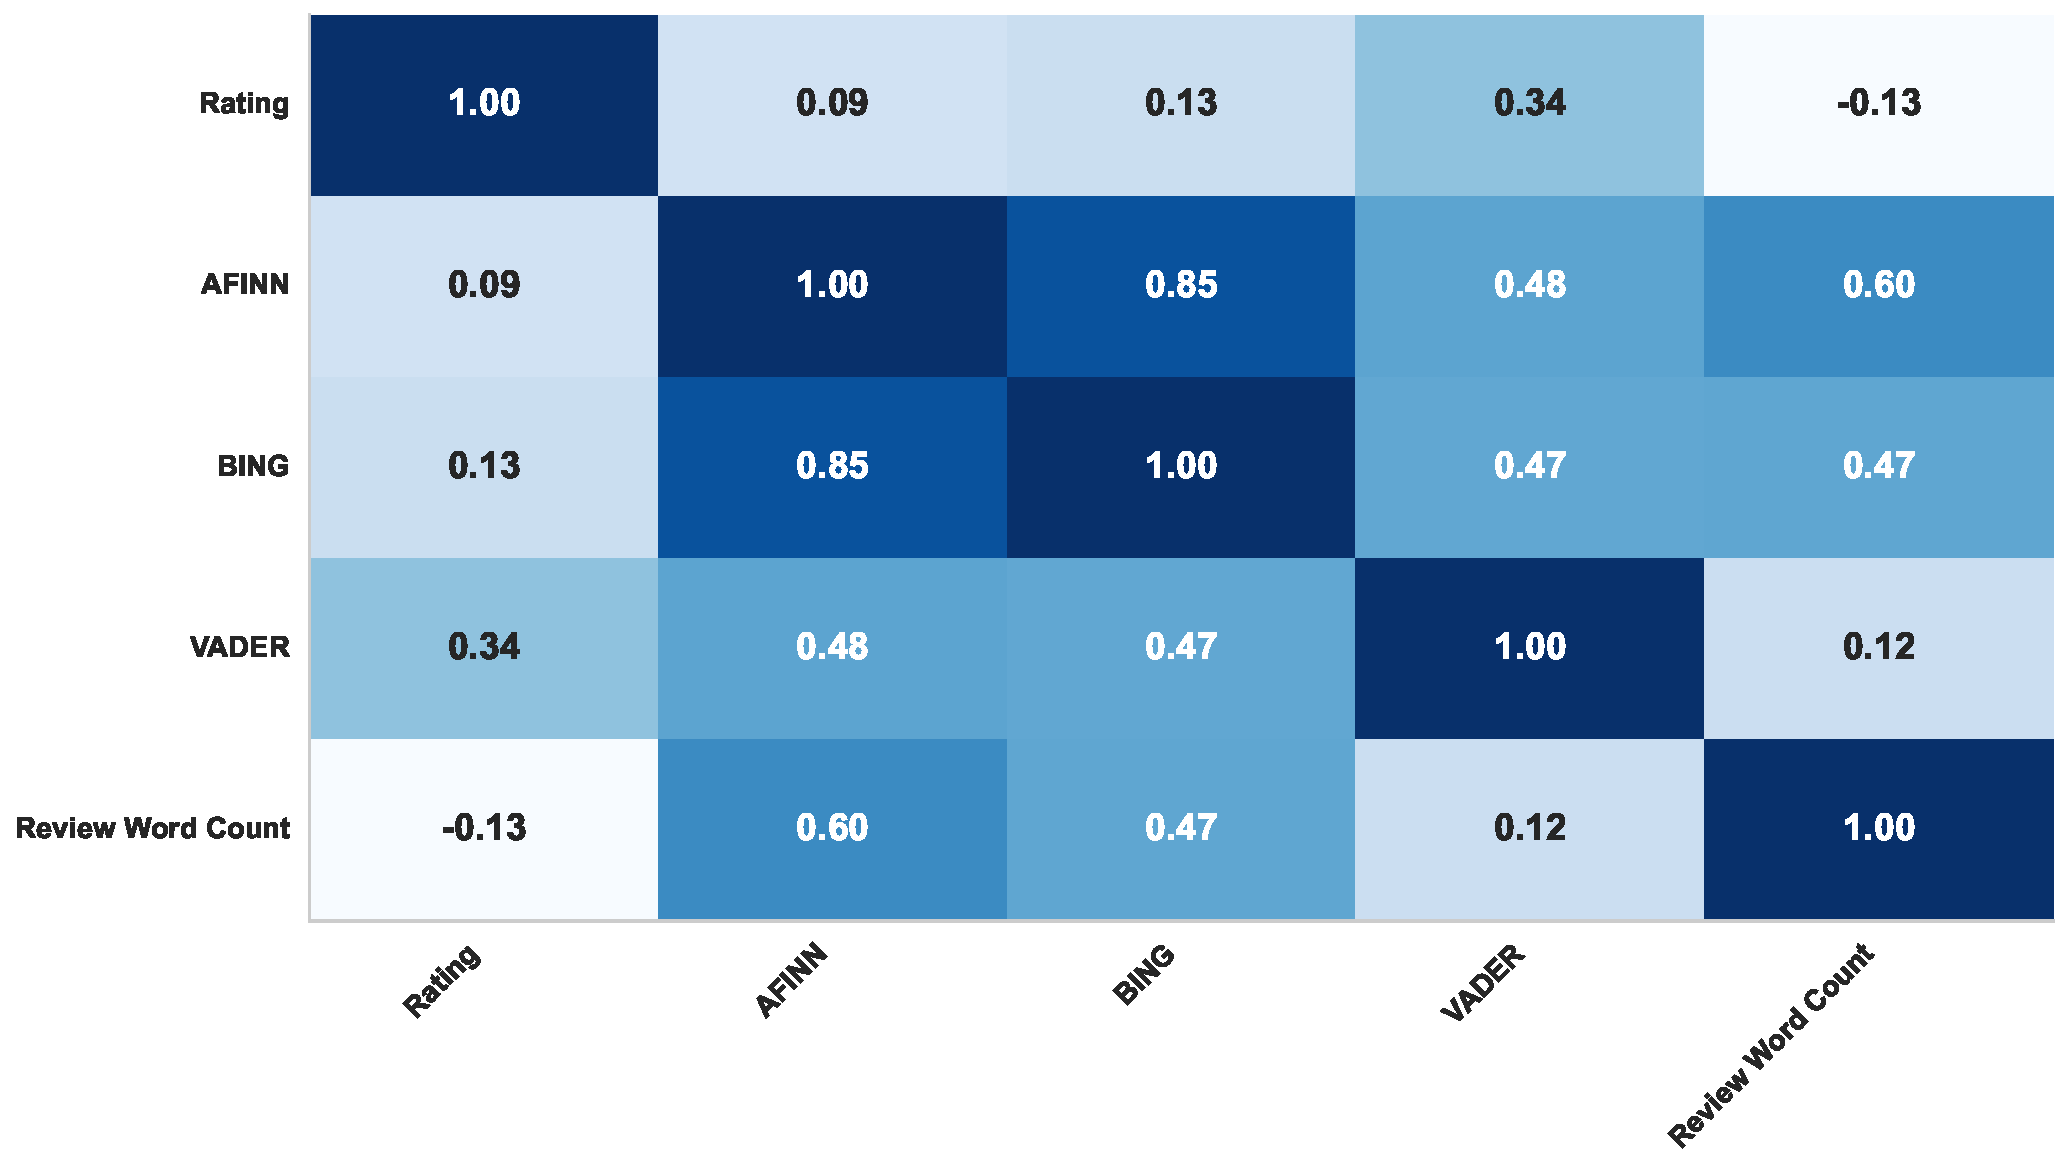
\includegraphics[width=0.9\textwidth]{Figures/correlation_between_ratings_sentiment_scores_review_length.pdf} % Adjust the width as needed
  \caption{Relationship Between Lexicon-Based Methods and Ratings.}
  \label{fig:correlation heat map sentiments}
\end{figure}


\section{Data Partitioning}
\label{sec:3 Data Partitioning}

When analysing a recommendation model, we are more concerned with its future performance on new (unseen) data, rather than in its performance on past data \cite{witten2005practical}. In order to test future performance and estimate the prediction error, we must properly partition the original dataset into training and test subsets. This section outlines the data partitioning strategy employed for this thesis, considering the cleaned and transformed reviews dataset consisting of over 250,000 records. 

Training data refers to the data that is used by one or more learning methods to develop the model and the test data is used to evaluate the quality of the model by giving the trained model this unseen (test) data \cite{witten2005practical}. The test set must be different and independent from the training set in order to obtain a reliable estimate of the true error \cite{witten2005practical}. It is very important that performance is estimated on data which take no part in the formulation of the model. Some learning schemes, such as in the case of ours, need also a validation set in order to optimise the model parameters. In summary, to evaluate the performance of our recommender models, we need to train, validate (to optimise) and test our recommender model using different data. To do so, is not as simple as randomly allocating reviews (records) into three distinct sets. 

For recommender systems, the partitioning is performed by randomly selecting some ratings from all (or some of) the users. That is, for each user, we randomly select some ratings they have given and hide them, whilst keeping their remaining ratings in tact and to be used for training. The selected ratings constitute the test set, while the remaining ones are the training set. This method is called leave-$k$-out\footnote{method involves selecting a subset of $k$ ratings from the dataset as the test set, while the remaining ratings form the training set}. In \cite{sarwar2002incremental}, they split the dataset into 80\% training and 20\% test data following this leave-$k$-out approach. In \cite{herlocker1999algorithmic} the test set is made by 10\% of users: here only 5 ratings for each user in the test set are withheld. This leave-$k$-out approach is in fact also the method that we employ in our paper. 

We opted to hide 3 random ratings from each user and allocate these to the test set, and 2 (again random) ratings to the validation set, and allocate the remaining reviews for the user to the training set. To further ensure the integrity of the partitioning process, we also ensured that the reviews for each user were randomly shuffled before allocating them to the respective subsets. This randomisation helps to mitigate any potential biases that may be present in the original dataset and ensures a representative distribution of user-item interactions across the subsets. We used a seed of 2207 to ensure reproducibility of the results. Note, there are other methods of splitting the dataset such as $k$-fold cross-validation\footnote{$k$-fold cross-validation divides the dataset into $k$ equally sized folds. The model is trained $k$ times, each time using $k-1$ folds for training and one fold for validation. The performance is then averaged over the $k$ iterations.}, however for our research we opted to use leave-$k$-out due to its simplicity and popularity in recommender research.

The choice for the partition was made to ensure that the recommender system is trained on a large enough dataset to capture the underlying patterns and relationships between users and items, whilst also ensuring that the test set is large enough to provide a reliable estimate of the model's performance. To that end, the training data, the largest partition of the data containing at least 9 reviews per user, comprises approximately 72 percent of the dataset, or close to 185 000 reviews. The validation set comprises of approximately 13 percent of the dataset (35,000 reviews. Finally, the test set is represented by approximately 13 percent of the dataset (35,000 reviews). These datasets are summarised in Table \ref{tab:partition summary}.

\begin{table}[h]
  \centering
  \begin{tabular}{|l|l|l|l|}
  \hline
  \textbf{Dataset} & \textbf{Purpose} & \textbf{Number of Reviews} & \textbf{Proportion of Reviews} \\
  \hline
  Training & Training the model  & 186 675 & 72.7\% \\
  \hline
  Validation & Model validation  & 35 025 & 13.64\% \\
  \hline
  Testing & Model evaluation  & 35 025 & 13.64\% \\
  \hline
  \end{tabular}
  \caption{Dataset Partition}
  \label{tab:partition summary}
  \end{table}

  The partitioning of the dataset into training, validation, and test sets is crucial for achieving reliable and accurate results. It helps to evaluate the recommender system's performance on unseen data and provides an estimate of its effectiveness in real-world scenarios. The training set facilitates the learning of user preferences, the validation set aids in fine-tuning the model, and the test set provides an independent assessment of the system's performance. Having established this partitioning process, our data is ready to be used for our analysis. 




\section{Conclusion}
\label{sec:3 Conclusion}

In this chapter we have discussed a variety of aspects of the Amazon product review dataset, ranging from data collection and preparation to exploratory data analysis and data partitioning for recommender systems. 

Specifically, in Section \ref{subsec:3 Amazon Review Dataset}, we provided some background and context on the Amazon Product Reviews dataset, which we have chosen for this thesis. In this same section we also dived into the details of the type of user feedback that we have in the dataset and explained that we are using explicit feedback provided through numerical ratings and review text variables. In section \ref{sec:3 Variable Description}, we provided a brief overview of the variables in the dataset and gave some descriptions of these. 

The data that consists of over 142 million reviews over an 18-year period. Through data management and filtering (see Section \ref{sec:3 Data Collection and Preprocessing}), we were able to extract a subset of the data that contains 91 235 reviews from 3801 unique users and 3283 unique products. In this same section, we also explained in detail the preprocessing steps taken to ready the data for further analysis, which included handling of nulls and duplicate amongst other steps. Subsection \ref{subsec:3 Text Analysis and Cleaning}and \ref{subsec:3 Sentiment Analysis} summarised the work done to analyse and clean the textual data - the user review text. These sections outlined the text cleaning steps taken from normalising  to lemmatising the review text. We also covered what sentiment analysis is (see Section \ref{subsec:3 Sentiment Analysis}) and why we opted for the VADER lexicon-based approach to generate the sentiment feature for the dataset. At this stage we had filtered our dataset to 83 139 reviews in the dataset, where we had 3668 unique users and 3249 unique products 

Sections \ref{sec:3 Data Summary} and \ref{sec:3 Trends and Patterns} provided a brief high level visual summary of the dataset from different angles, looking at user engagement, review text and ratings data. We looked at the distributions and identified any trends in the data. Over the entire cleaned data set of reviews (approximately 83 139 reviews), the average ratings are 4.4 - where the ratings are on a five-point scale. We also identified that the general sentiment of users vary, however they are majority positive. Lastly, we outlined the method of partition of our dataset in Section \ref{sec:3 Data Partitioning}. Data partitioning is a pivotal step in the development and evaluation of recommender systems, serving to gauge the system's ability to generalise to unseen user-item interactions. We opted for the leave-$k$-out approach where we simply, hid or removed 5 ratings at random from each user and allocated 2 of those hidden ratings to a validation set and 3 of them to a testing set, the balance of the ratings were used as the training set. 

As we transition to the next chapter on methodology, we build upon this foundational understanding of the dataset to look into the intricacies of our approach for building and evaluating recommender systems.

 \chapter{Methodology} % Main chapter title
\label{Chapter4}





\section{Modelling Approach}
\label{sec:Modelling Approach}

\subsection{Formulating the Problem}
\label{subsec:Formulating the Problem}

\subsection{Implementation and Approach}
\label{subsec:Implementation and Approach}























\section{Neural Collaborative Filtering}
\label{sec:Neural Collaborative Filtering}

\subsection{Background}
\label{subsec:Background}

\subsection{Algorithm Formulation}
\label{subsec:Algorithm Formulation for NCF}

\subsubsection{User and Item Embeddings}
\label{subsubsec:User and Item Embeddings}

\subsubsection{Neural Network Architecture}
\label{subsubsec:Neural Network Architecture}

\subsubsection{Loss Function}
\label{subsubsec:Loss Function}


\subsection{Algorithm Summary}
\label{subsec:Algorithm Summary}

\subsubsection{Model Training}
\label{subsubsec:Model Training}

\subsubsection{Hyperparameter Tuning}
\label{subsubsec:Hyperparameter Tuning}

\subsection{Incorporating Text and Sentiments}
\label{subsec:Incorporating Text and Sentiments}

\subsubsection{User Review Text}
\label{subsubsec:User Review Text}

\subsubsection{User Review Sentiments}
\label{subsubsec:User Review Sentiments}


\subsection{Training Results}
\label{subsec:Training Results}

\subsection{Final Model Specifications}
\label{subsec:Final Model Specifications}

\subsection{Summary}
\label{sec:Summary for NCF}

\section{Benchmark Models}
\label{sec:Benchmark Models}

\subsection{Non-Negative Matrix Factorisation}
\label{subsec:Non-Negative Matrix Factorisation}

\subsubsection{Algorithm Formulation}
\label{subsubsec:Algorithm Formulation}

\subsubsection{Adjusting for Sparsity and Regularisation}
\label{subsubsec:Adjusting for Sparsity and Regularisation}


\subsubsection{Algorithm Summary}
\label{subsubsec:Algorithm Summary}



\subsubsection{Adjusting for Bias}
\label{subsubsec:Adjusting for Bias}


\subsection{Item-Based Collaborative Filtering}
\label{subsec:Item-Based Collaborative Filtering}


\subsubsection{Algorithm Formulation}
\label{subsubsec:Algorithm Formulation}

\subsubsection{Algorithm Summary}
\label{subsubsec:Algorithm Summary}


\subsection{User-Based Collaborative Filtering}
\label{subsec:User-Based Collaborative Filtering}


\subsubsection{Algorithm Formulation}
\label{subsubsec:Algorithm Formulation}


\subsubsection{Algorithm Summary}
\label{subsubsec:Algorithm Summary}

\section{Evaluation}
\label{sec:Evaluation}


\subsection{Evaluation Approach}
\label{subsec:Evaluation Approach}


\subsubsection{Predictive Accuracy}
\label{subsubsec:Predictive Accuracy}


\subsubsection{Top-N Evaluation}
\label{subsubsec:Top-N Evaluation}


\subsection{Evaluation Metrics}
\label{subsec:Evaluation Metrics}

\subsubsection{MSE, RMSE and MAE}
\label{subsubsec:MSE, RMSE and MAE}


\subsubsection{HR and NDCG}
\label{subsubsec:HR and NDCG}


\section{Conclusion}
\label{sec:Conclusion for Methodology}
 
 % Chapter Template

\chapter{Model Specification and Analysis} % Main chapter title

\label{Chapter5} % Change X to a consecutive number; for referencing this chapter elsewhere, use \ref{ChapterX}



\begin{figure}[h]
\centering
  \includegraphics[scale =0.9]{/Users/pavansingh/Google Drive (UCT)/STA Honours/Project/Thesis/Python Coding/Figures/Methods/Untitled Diadsdsdsgram.pdf}
  \caption{Diagram illustrating the models and whole experimental procedure followed.}
  \label{}
\end{figure}

All 42 variables, including mix of stock data (open, high, low, close and volume), as well several technical indicators. were used as inputs to our. models. Our feed-forward and long-short term memory neural networks were configured as classification models, while our ensemble trees, where configured as regression problems. As such, since we want to assess these models on their ability to predict the movements of daily log returns of stocks, we had to convert our predictions from our ensemble models to binary output. This was done, by coding returns equal to or greater than zero as one and any negative returns as zero.

%----------------------------------------------------------------------------------------
%	SECTION 1
%----------------------------------------------------------------------------------------

\section{Model Architectures}

Hyper-parameters are the parameters that are set prior to the learning process (Nelson \textit{et al.}, 2017). They are not derived via training. Hyper-parameter optimisation allows for improving and - in some cases - correcting an algorithm’s performance. One of the main characteristics to consider when optimising hyper-parameters is the model's complexity (Nti \textit{et al.}, 2020). If the model is over-complex, it might be prone to overfitting and thus will not generalise well. On the other hand, if it is too simplistic, the model might not fit the data correctly or be able to capture the relationship between input and output sufficiently under-fitting (Nelson \textit{et al.}, 2017).

There are several approaches to find the model hyper-parameters that yield the best score on the validation set metric. In our paper, we opted for using a grid search and in some cases,  manually searching for optimal hyper-parameters. 

\subsection{Long Short-Term Memory Neural Network}

The network is based on a sequential model. We used a cross validation grid search \footnote{Grid Search CV tries all combinations of parameters grid for a model and returns with the best set of parameters having the best performance score} from Scikit-Learn module to try out several values for our hyper-parameters and compare the results. 

Hyper-parameters tuned with grid search, with the accompanied combination of values tried, is shown in the table below.

\begin{table}[h]
\centering
\begin{tabular}{ll}
\hline
Hyper-parameter     &  Value \\
\hline
Batch Size      & 4, 12, 24 \\
Dropout & 0.2, 0.3, 0.4 \\
Learning Rate & 0.1, 0.01, 0.001 \\
LSTM Units & 20, 50, 100 \\
Dense Units & 1, 5, 20\\
\hline
\end{tabular}
\caption{Hyper-Parameters and their corresponding combination of values used in grid search for our LSTM.}
\end{table}

\begin{itemize}
\item  \verb|batch_size|: defines the number of samples that will be propagated through the network
\item  \verb|dropout|: a regularisation technique, which helps with reducing overfitting
\item  \verb|LSTM units|:  number of neurons in a LSTM layer
\item  \verb|Dense units|:  number of neurons in dense layers
\item \verb|Learning Rate|: controls how much to change the model in response to the estimated error each time the model weights are updated
\end{itemize}

Our final model has two LSTM layers, each followed by a dropout layer with dropout value of 0.2. Dropout is a regularisation technique for neural network, where randomly selected neurons are ignored during training. As such, the contribution of those selected neurons to the activation of downstream neurons is temporally removed on the forward pass. Thus any weight updates are not applied to the neuron on the backward pass. Ultimately,  this helps in reducing the possibility of over-fitting the network (Nelson \textit{et al.}, 2017). In addition, we have two dense layers in our model architecture. The dense layer is the most frequently used layer which is basically a layer where each neuron receives input from all neurons in the previous layer (Nelson \textit{et al.}, 2017). 

The loss function used was the binary cross entropy function - as it was appropriate the type of problem we have - supervised binary classification. With regards to the number of neurons (units) in the hidden layers, there is no straightforward approach one should use. We chose to grid search with 20, 50 and 100 units in the LSTM layers. The final model has 100 units in the LSTM layer.  

With respect to the models fit and architecture, we also consider the activation function and choice of optimiser. We used both a rectified linear unit (ReLU) and sigmoid activation function in the final model architecture. The ReLU activation function is specified for all except the output layer. The sigmoid activation function is used in the final output layer, satisfying our binary classification solution. The optimiser used for this model was stochastic gradient descent (SGD). 

Our grid search results suggested we use a learning rate of 0.01. We note that setting a higher learning rate accelerates the learning but the model may not converge. Conversely, a lower rate will slow down the learning drastically as steps towards the minimum of loss function will be tiny, but will allow the model to converge smoothly.  Finally, we specified 100 epochs \footnote{the number of iterations (forward and back propagation) our model needs to make.} and set a stopping method, which stops training once the model performance stops improving by a pre-set threshold on the validation set. The final model architecture is summarised in the table below:

\begin{table}[h]
\centering
\begin{tabular}{ll}
\hline
Hyper-parameter     &  Value \\
\hline
Epochs     & 100  \\
Batch Size      & 12 \\
Dropout & 0.2 \\
Dropout Layers & 2 \\
Activation Function & ReLU and Sigmoid \\
Learning Rate & 0.01 \\
Optimiser & Binary Cross Entropy \\
LSTM Units & 100\\
LSTM Layers & 2\\
Dense Layers & 2\\
Dense Units & 5 and 1 \\
\hline
\end{tabular}
\caption{Chosen hyper-parameters for LSTM. We used a grid search with cross validation to select the number of units in the LSTM layer, the dropout, learning rate and batch size.}
\end{table}


A rectified linear unit (ReLU) function is written as: 
\begin{equation}
f(x)=\left\{\begin{array}{ll}
0 & \text { if } x \leq 0 \\
x & \text { otherwise }
\end{array}\right.
\end{equation}

The ReLU activates a node with the same input value only when the input is above zero.




\subsection{Feed-Forward Neural Network}

The hyper-parameters for our feed-forward neural network (FFNN), are similar to that of our LSTM model. However, we do not have dropout layer nor do we have LSTM layers in our architecture for the FFNN.  We again used a grid search with cross validation from Scikit-Learn module to try out several values for our hyper-parameters and compare the results. The combination of values in the grid are shown in Table 5.3.

\begin{table}[h]
\centering
\begin{tabular}{ll}
\hline
Hyper-parameter     &  Value \\
\hline
Batch Size      & 4, 12, 24 \\
Learning Rate & 0.1, 0.01, 0.005, 0.001 \\
Dense Units & 1, 10, 20, 50\\
\hline
\end{tabular}
\caption{Hyper-Parameters and their corresponding combination of values used in grid search for our FFNN.}
\end{table}


For our optimisation algorithm, we again opted for SGD. We tuned the learning rate, and found that 0.01 produced the best model performance on the validation set. The selection of the rest of our hyper-parameters, as well as the final model architecture is shown in table 5.4. 



\begin{table}[h]
\centering
\begin{tabular}{ll}
\hline
Hyper-parameter     &  Value \\
\hline
Epochs       & 100  \\
Batch Size      & 0.01 \\
Activation Function & 1 (default) \\
Learning Rate & 1 (default) \\
Optimiser & 1 (default) \\
Dense Layers & 2\\
Dense Units & 5, 1\\
\hline
\end{tabular}
\caption{Chosen Hyper-Parameters for FFNN. We used a grid search with cross validation to select the number of units in the dense layers, the learning rate and batch size.}
\end{table}


\subsection{Random Forest}

The hyper-parameters for our random forest were found by implementing a grid search with cross validation as well. The hyper-parameters we are concerned with for this model include:
\begin{itemize}
\item \verb|n_estimators|: the number of decision trees in the forest
\item  \verb|max_features|: max number of features considered for splitting a node
\item  \verb|max_depth|: max number of levels in each decision tree
\item  \verb|min_samples_split|:  number of data points placed in a node before the node is split
\end{itemize}

By building forests with a large number of trees (high number of estimators) we can create a more robust aggregate model with less variance. This comes at the cost of a greater training time (Ampomah \textit{et al.}, 2020). We also note that due to the randomness of Random Forests, if you have a lot of features and a small number of trees some features with high predictive power could get left out of the forest and not be used whatsoever (Ampomah \textit{et al.}, 2020). 

With respect to the maximum features considered at each node split, we have to be careful in deciding upon a value.  A small value (less features considered when splitting at each node) will reduce the variance of the ensemble, at the cost of higher individual tree bias (Nti \textit{et al.}, 2020). Increasing the maximum number of random features considered in a split tends to decrease the bias of the model, as there is a better chance that good features will be included, however this can come at the cost of increased variance. Given that we have many features we chose a combination of values for this parameter, shown in figure 5.2. For max depth of trees, if we increase this value,  this would increase the possible number of feature combinations that are taken into account. The deeper the tree, the more splits it has and the more information about the data it takes into account (Ampomah \textit{et al.}, 2020).

\begin{figure}[h]
\centering
  \includegraphics[scale =0.37]{/Users/pavansingh/Google Drive (UCT)/STA Honours/Project/Thesis/Python Coding/Figures/RF AND BOOST/VAL/RandomForestGRID.pdf}
  \caption{Grid search results using different combination of values for hyper-parameters of Random Forest. We select a max depth of 20 and minimum sample split of 2.}
  \label{}
\end{figure}

Figure 5.2 depicts the optimal hyper-parameters for our Random Forest model on the validation set. It can be observed, that as the maximum depth of the decision tree increases and as minimum sample leaf decreases, the algorithm tend to overfit. This results in an optimistic training-validation set performance and decreased generalisation performance on the test set. Thus, in order to obtain the best performing model, we need to determine both the optimal tree depth as well as the minimum sample leaves at the same time. After hyper-parameter tuning, we were able to obtain the parameters for our final Random Forest model. These can be seen in table 5.5.

 
\begin{table}[h]
\centering
\begin{tabular}{ll}
\hline
Hyper-parameter   &  Value \\
\hline
Max Number Estimators       & 250  \\
Max Depth & 20 \\
Min Samples Split & 2 \\
\hline
\end{tabular}
\caption{Chosen model hyper-parameters for Random Forest model. We found the minimum samples split and max depth, by implementing a cross validation grid search.}
\end{table}




\subsection{AdaBoost Model}

Similar to our Random Forest, we need to specify the number of estimators for our AdaBoost algorithm. That is, the maximum number of estimators (trees) at which boosting is terminated. In contrast to Random Forests, we have to specify a learning rate - how fast the tree learns. 

We also have to specify the base estimator. The default value is none, which equates to a decision tree with max depth of 1 (a stump). For the hyper-parameters of our AdaBoost model we applied a grid search over a combination of values. The results of which are shown in figure 5.3. 

\begin{figure}[h]
\centering
  \includegraphics[scale =0.34]{/Users/pavansingh/Google Drive (UCT)/STA Honours/Project/Thesis/Python Coding/Figures/RF AND BOOST/VAL/Best_Model_Boosting_2.pdf}
  \caption{Grid Search Results using Different Combination of Values for Hyper-parameters of Adaboost Model. The chosen hyper-parameters, were a max depth of ten and minimum samples leaf of ten.}
  \label{}
\end{figure}

We chose to vary the learning rate to penalise our model against overfitting. The results of using a learning rate of 0.01 and 1 are shown in the appendix C. After hyper-parameter tuning, we were able to obtain the parameters for our final model. These can be seen in the Table 5.6.

\begin{table}[h]
\centering
\begin{tabular}{ll}
\hline
Hyper-parameter     &  \\
\hline
Max Number Estimators       & 250  \\
Learning Rate        & 0.01 \\
Max Depth & 1 (default) \\
\hline
\end{tabular}
\caption{Chosen Hyper-Parameters for AdaBoost Model}
\end{table}

For both ensemble decision tree models, we constructed regression trees. We predicted the daily log eturns to infer the movement of the stocks. Our binary prediction was set such that zero indicated a negative return and a one indicated a positive return.


\newpage
\subsection{Auto Regressive Integrated Moving Average}

The modelling procedure for fitting our ARIMA model is as follows (): 

\begin{itemize}
\item Plot the data and identify any unusual observations.
\item If necessary, transform the data (using a Box-Cox transformation) to stabilise the variance.
\item If the data are non-stationary, take first differences of the data until the data are stationary.
\item Examine the ACF/PACF: Is an ARIMA $(p, d, 0)$ or ARIMA $(0, d, q)$ model appropriate?
\item Try your chosen model(s), and use the AIC to search for a better model.
\item Check the residuals from your chosen model by plotting the ACF of the residuals, and doing a portmanteau test of the residuals. If they do not look like white noise, try a modified model.
\item Once the residuals look like white noise, calculate forecasts.
\end{itemize}

As such, we used AIC to determine the order of the ARIMA model (Binner \textiot{et al.}, 2005). AIC is written as: 

\begin{equation}
\mathrm{AIC}=-2 \log (L)+2(p+q+k+1), 
\end{equation}

where $L$ is the likelihood of the data, $k=1$ if $c \neq 0$ and $k=0$ if $c=0$. Good models are obtained by minimising the AIC. 
We looked at a combination of different p and q values. The results of our analysis are shown in the table below:

\begin{table}[h]
\centering
\begin{tabular}{ll}
\hline
Model Specification & AIC        \\
\hline
(1, 0, 1)           & -10549.128 \\
(1, 0, 0)           & -10545.228 \\
(2, 0, 0)           & -10551.196 \\
(2, 0, 2)           & -10551.033 \\
(3, 0, 1)           & -10548.880 \\
(2, 0, 1)           & -10554.112 \\
\hline
\end{tabular}
\caption{Combination of different ARIMA model specifications used to find the optimal architecture}
\end{table}

Of these models shown in Table 5.7, the ARIMA(2,0,1) has the smallest AIC value, hence it is our chosen model. Figure 5.3 shows the residual diagnostic plots from the ARIMA(2,0,1) model. 

\begin{figure}[h]
\centering
  \includegraphics[scale =0.34]{/Users/pavansingh/Google Drive (UCT)/STA Honours/Project/Thesis/Python Coding/Figures/ARIMA/DiagnosticsARIMA_301_FORD.pdf
}
  \caption{Model diagnostics for the ARIMA(2,0,1) model.}
  \label{}
\end{figure}

We see from the plot in the top right of figure 5.4, that. the residuals have a mean close to 0.  Pots in figure 5.4 shows that all autocorrelations are within the threshold limits, indicating that the residuals are behaving like white noise. Any autocorrelation would imply that there is some pattern in the residual errors which are not explained in the model. 

We note that the QQ-plot indicates that the distribution of the residuals deviate from normality in the tails.  We apply the Box-Ljung test \footnote{Tests whether any of a group of autocorrelations of a time series are different from zero. Null hypothesis is that the data are random.} to the residuals from the ARIMA(2,0,1) model fit to determine whether residuals are random. We received a p-value of 0.008 indicating that the residuals are random and that the model provides an adequate fit to the data. The top left plot in figure 5.4, illustrates the standardised residuals.  These residual errors seem to fluctuate around a mean of zero and for the most part have a uniform variance. 


%----------------------------------------------------------------------------------------
%	SECTION 1
%----------------------------------------------------------------------------------------

\section{Validation Analysis}

The validation data set provides an un-biased evaluation of a model fit on the training data set while tuning the model's hyper-parameters. Using our optimised models, we illustrate the validation curves for our LSTM and FFNN models on the Ford Motors stock.

The loss (or cost) measures our model error. Specifically, the training loss indicates how well the model is fitting the training data, while the validation loss indicates how well the model fits new data.  

%\begin{figure}[h]
%\centering
%  \includegraphics[scale =0.30]{/Users/pavansingh/Google Drive (UCT)/STA Honours/Project/Thesis/Python Coding/Figures/ANN/LOSS/ModelLoss_ANN_Google.pdf}
%  \caption{Loss Curve for Tuned LSTM Network on Ford Data.}
  %\label{}
%\end{figure}

\begin{figure}[h]
    \centering
    \subfloat[Multivariate LSTM]{\label{fig:2:a}\includegraphics[width=0.5\textwidth]{/Users/pavansingh/Google Drive (UCT)/STA Honours/Project/Thesis/Python Coding/Figures/ANN/LOSS/ModelLoss_ANN_Google.pdf}}
    \subfloat[Multivariate FFNN]{\label{fig:2:b}\includegraphics[width=0.5\textwidth]{/Users/pavansingh/Google Drive (UCT)/STA Honours/Project/Thesis/Python Coding/Figures/ANN/LOSS/ModelLoss_ANN_Ford.pdf}}    
\label{}
\end{figure}


We note that the loss curve for our training data decreases quickly over each iteration, and flattens out after around 6 iterations. Similarly, we see that our validation curve decreases as we iterate through the data. The validation curve reaches the training loss curve at the 9th iteration. After the 12th iteration the validation curve flattens. 

%\begin{figure}[h]
%\centering
%  \includegraphics[scale =0.30]{/Users/pavansingh/Google Drive (UCT)/STA Honours/Project/Thesis/Python Coding/Figures/ANN/LOSS/ModelLoss_ANN_Ford.pdf}
%    \caption{Loss Curve for Tuned FF Network on Ford Data.}
%  \label{}
%\end{figure}

%----------------------------------------------------------------------------------------
%	SECTION 1
%----------------------------------------------------------------------------------------

\section{Variable Feature Importance}

The feature importance captures how much the splits produced by the feature helped to optimise the model's metric used to evaluate the split quality, which in our case is the mean square error (Ampomah \textit{et al.}, 2020). 


\begin{figure}[h]
        \begin{adjustwidth}{-1.2cm}{}

    \subfloat{\label{fig:2:f}\includegraphics[width=0.55\textwidth]{/Users/pavansingh/Google Drive (UCT)/STA Honours/Project/Thesis/Python Coding/Figures/RF AND BOOST/BOOST_importance.pdf}}
     \subfloat{\label{fig:2:f}\includegraphics[width=0.55\textwidth]{//Users/pavansingh/Google Drive (UCT)/STA Honours/Project/Thesis/Python Coding/Figures/RF AND BOOST/RF_importance.pdf}}
    \caption{\small{Variable importance plots from our ensemble decision tree models. }}
\label{}
 \end{adjustwidth}    

\end{figure}



Across both of our models we see that Moving Average Convergence Divergence (MACD) was the most significant predictive variable. Coincidentally, this happens to be one of the most popular technical indicators used in practice. The MACD is a trend following momentum indicator which shows the relationship between two different moving averages on our stocks price. It essentially serves as a signal to indicate when a price has risen/dropped by too much and will correct back to its 26- day moving average. In addition, another strongly predictive feature was the 21-day Exponential Moving Average (EMA). Essentially, an EMA is just a moving average of a stock’s returns where the last few days are given larger weights (Ampomah \textit{et al.}, 2020).


%----------------------------------------------------------------------------------------
%	SECTION 1
%----------------------------------------------------------------------------------------

 
  % Chapter Template

\chapter{Conclusion} % Main chapter title
\label{Chapter6} % Change X to a consecutive number; for referencing this chapter elsewhere, use \ref{ChapterX}

In Chapter \ref{Chapter5}, we looked into the results from this thesis and their implications concerning our research questions, including a deeper discussion of what was observed from our analysis in general. In this chapter, we aim to offer a comprehensive overview of the primary findings derived from this thesis, representing the culmination of our analysis, and outlining their implications moving forward.

The chapter begins with an overview of the results in Section \ref{sec:6 Summary of Results and Findings}. Following this, Section \ref{sec:6 Limitations} addresses the limitations of the thesis, both from a perspective of limited experimentation, as well as from a perspective of the various assumptions made. These identified shortcomings pave the way for Section \ref{sec:6 Future Work}, which explores potential avenues for further exploration or enhancement of the methodologies employed. Finally, we draw this thesis to a close with Section \ref{sec:6 Conclusion for Conclusion}, which serves to summarise and raise key points to conclude this thesis. 


\section{Summary of Results and Findings}
\label{sec:6 Summary of Results and Findings}


In Section \ref{sec:5 Results}, we evaluated the results from our study for two problems: rating prediction and top-$n$ generation. We summarise the key findings from our study. 



\textbf{Rating Prediction}
\begin{itemize}
    \item The NCF model outperformed all benchmark models across all predictive accuracy metrics, including MAE, RMSE, and MSE.
    \item The review-aware NCF model, integrating ratings and review text, exhibited the best performance, achieving an MAE of 0.490 and RMSE of 0.769.
    \item The inclusion of sentiment analysis alongside reviews marginally decreased performance, resulting in marginally higher RMSE and MAE values (MAE of 0.492 and RMSE of 0.779).
    \item A one-sample paired t-tests showed that there is evidence that the NCF model significantly outperforms all benchmark models at a significance level of $p<0.01$.
    \item Users with more reviews had lower MAE and RMSE values, indicating that the NCF model performed better for users with more reviews.
    \item The predictive accuracy did not change significantly for items with more reviews, indicating that the NCF model performed similarly for items with varying review counts.
    \item  Reviews with fewer words had lower MAE and RMSE values, indicating that the NCF model performed better for reviews with fewer words.
    \end{itemize}
    

\textbf{Top-$N$ Generation}
\begin{itemize}
    \item The NCF model struggled to recommend relevant products for users' top-$n$ recommendations, particularly within the Top-100 list.
    \item All models performed poorly on the top-$n$ tasks, although the NCF model outperformed the benchmarks models.
\end{itemize}


\textbf{Computational Details}
\begin{itemize}
    \item The NCF model with review text and sentiments required only 13 minutes for model training
    \item The slowest NCF model, NCF model with reviews, was quicker (13 minutes) than the fastest benchmark model, user-based collaborative filtering (125 minutes).
    \item NMF took the longest runtime at 457 minutes.
    \item The efficiency of the NCF models was particularly noteworthy with respect to computation, with shorter run-times compared to benchmark models, even when augmented with additional information such as review text and sentiments. Largely attributed to using TensorFlow for NCF, whilst the benchmark models were built from scratch.
\end{itemize}


Directly addressing our research questions, the incorporation of review text enhanced rating prediction performance within recommender systems. However, the addition of sentiments did not yield further improvements. Moreover, the efficacy of the NCF models was evident, performing better than all the benchmark models across the predictive accuracy metrics used. Furthermore, the efficiency of the NCF models was particularly noteworthy with respect to computation, with shorter run-times compared to benchmark models, even when augmented with additional information such as review text and sentiments. 


\section{Limitations}
\label{sec:6 Limitations}

In building our recommender system, our primary focus centered on rating predictions aimed at minimising the disparity between actual and predicted ratings. The overarching goal was to develop a recommendation system capable of accurately predicting unknown ratings for items, leveraging a training set to discern user preferences, and assessing the system's efficacy by evaluating its performance on a testing set containing concealed ratings provided by users for various items. This evaluation process involved measuring predictive accuracy metrics such as RMSE and MAE. Having achieved predicted ratings for all unrated items for each user we were able to identify a list of items (top-$n$) by sorting the ratings for unrated items to identify a top-$n$ list of recommendations for each user. We measured this list using metrics such as recall@$n$ and precision@$n$. The results of which were not impressive. In hindsight, these observations shed light on several limitations inherent in our study, prompting a critical re-evaluation of our methodologies and approaches.

Firstly, we built the model for a specific goal - rating prediction, however we tested its capability on different task - top-$n$ generation. We have established that there is no one universal recommender system \cite{lu2012recommender} and that a recommender's performance is not transferable from one objective to another. Consequently, the results obtained from the top-$n$ generation task offer limited insights into the effectiveness of our review-aware NCF model in this specific use case. Indeed, while our recommender system performed relatively well in predicting ratings for unknown products, its performance in generating top-$n$ recommendations was considerably less satisfactory. That is to say, we observed that the model struggled to recommend relevant (items in test set) products for a users Top-100. In fact, the performance was not better than random recommender. Thus, given the misalignment between the model's training objective and the evaluation task, the results obtained from the top-$n$ generation task should be interpreted with caution, and the conclusions drawn from them should be viewed in light of this limitation. 

To that end, the misalignment between the training objective and the evaluation task underscores the importance of aligning the recommender system's training and evaluation objectives to ensure that the model is optimised for the task at hand. With the evolving understanding that recommendation accuracy alone does not guarantee an effective and satisfying user experience, our approach of generating a recommender solely for predicting unrated items provides a limited scope for building a good or useful recommender system. To address this limitation, it becomes imperative to extend beyond simple accuracy metrics and optimise recommenders for tasks beyond rating prediction. This necessitates a more nuanced evaluation approach that encompasses multiple dimensions of performance, rather than focusing solely on rating prediction accuracy. Such multi-objective recommenders can be designed to optimise for a range of criteria, including diversity, novelty, serendipity, and user satisfaction, thereby ensuring a more comprehensive recommendation capability. 


Another key challenge and limitation encountered in this study pertained to the computational resources allocated to meet the thesis's requirements. For loading and handling the dataset, we relied on our local machine, which presented several challenges in managing the data effectively and efficiently. Thus, we limited our dataset by sampling records from the original repository, which contained over 140 million records. Additionally, we further restricted the dataset to users with 13 or more ratings and items with 13 or more reviews. While these constraints were necessary to ensure the feasibility of our analysis on the local machine, they also introduced limitations that may have impacted the performance and utility of our recommender system. 

With respect to the computational restrictions, beyond dataset handling, the model building and training occurred on our local machine, which inhibited the path of additional experimentation. Despite our efforts, all the benchmark models were restricted (due to their excessive run-times and memory allocations) in their tuning capabilities, with hyperparameter adjustments limited to only two or three options for each parameter. While it is not expected that the performance will be substantially improved had we been able to perform a more extensive hyperparameter search, it could be worthwhile trying to quantify how much improvement can be gained by performing a large hyperparameter search as compared to using a standard set of hyperparameters. Additionally, we compared an NCF model with extensive hyperparameter tuning with benchmark models that had minimal hyperparameter tuning. This comparison could have been more equitable had we performed a more extensive hyperparameter search for the benchmark models. Ultimately, the computational constraints as well as the limited time dictated a lot of the decisions made in the methodology. This challenge also touches upon a broader issue of scalability, an aspect that was acknowledged in Section \ref{subsec:2 Scalability} but was not addressed within the scope of this thesis. Nonetheless, given the context of the recommender system within e-commerce, scalability emerges as a primary concern. Addressing this concern could significantly enhance the run-times of benchmark models, particularly matrix factorisation approaches, by leveraging packages specifically designed to handle the inherent sparsity of the user-item matrix. The benchmark models, detailed in Section \ref{sec:4 Benchmark Models}, were constructed from scratch in Python, with minimal effort directed towards mitigating scalability issues or managing the computational overhead of training. 

One final limitation inherent in our thesis is the omission of addressing the cold start problem. We chose to mitigate the cold start problem, or rather circumvent it entirely, by restricting the dataset to users with 13 or more ratings and items with 13 or more reviews. While this approach provides a starting point, it limits the generalisability of our findings and the applicability of our recommender system to real-world scenarios. The cold start problem is a pervasive challenge in recommender systems, particularly for new users or items with limited interaction history. Addressing this challenge requires the development of innovative strategies to handle users or items with limited historical data. While the cold start problem was not the primary focus of our study, it represents a critical limitation that warrants further exploration and consideration in future research.


\section{Future Work}
\label{sec:6 Future Work}

\subsection{Developing Multi-Objective Recommender Systems}
\label{subsec:6 Multi-Objective Recommender Systems}

We have stablished the importance of a comprehensive evaluation approach to recommender systems, one that extends beyond rating prediction accuracy to encompass a broader range of performance metrics. Avenues for developing multi-objective recommenders that optimise for diverse criteria, including diversity, novelty, serendipity, and user satisfaction, represent a promising direction for future research. By adopting a more holistic evaluation approach, recommender systems can be designed to cater to a wider range of user preferences and needs, thereby enhancing the overall user experience. This approach aligns with the evolving understanding that recommendation accuracy alone does not guarantee an effective and satisfying user experience, underscoring the need for a more nuanced evaluation framework that captures the multifaceted nature of recommender systems. Various strategies can be employed to address this, including direct enhancement of recommendation list diversity and the integration of hybrid recommendation methods to meet different task objectives (\cite{smyth2001similarity};\cite{ziegler2005improving};\cite{hurley2011novelty};\cite{zhou2010solving}). Ultimately, future endeavors should prioritise the adoption of a more comprehensive approach to developing multi-objective recommender systems,and hence, evaluating recommenders based on a broader range of performance metrics.

\subsection{Enhancing Neural Collaborative Filtering with NeuMF}
\label{subsec:6 Enhancing Neural Collaborative Filtering with NeuMF}

The development of our NCF was based off the framework established by \cite{he2017neural}. The findings from our analysis underscored the improvements in predictive accuracy achieved by the NCF model when compared to conventional collaborative filtering methods. The work in this thesis can be extended to hybridising the architecture of NCF by incorporating matrix factorisation, resulting in the algorithm Neural Matrix Factorisation (NeuMF) - as detailed by \cite{he2017neural}. The rationale behind this approach stems from the recognition that traditional matrix factorisation can be viewed as a specialised instance of NCF. Therefore, by fusing the neural interpretation of matrix factorisation with Multilayer Perceptron (MLP), NeuMF emerges as a more generalised model harnessing the linearity of matrix factorisation and the non-linearity of MLP to enhance recommendation quality. Notably, the empirical findings from studies such as \cite{zhang2019deep} and \cite{he2017neural} corroborate the performance benefits offered by NeuMF over NCF. This naturally extends our comparative analysis, inviting us to integrate and adapt the advancements put forth by \cite{he2017neural} to incorporate NeuMF into our framework. This avenue for future can further be extended by investigating the augmentation of review text and sentiments within this enhanced framework — an area that, to the best of our knowledge, has not yet been explored.


\subsection{Exploring Advanced Word Embedding and Sentiment Analysis Techniques}

For our analysis, we employed a simple word embedding technique (USE) to convert review text into numerical vectors, which were subsequently integrated into our NCF model. However, the choice of word embedding technique can significantly impact the performance of the recommender system \cite{asudani2023impact}, with advanced methods such as Word2Vec, GloVe, and BERT offering more sophisticated representations of textual data (\cite{mikolov2013distributed}; \cite{pennington2014glove}; \cite{devlin2018bert}). Therefore, it stands to reason that exploring additional word embedding techniques beyond the simple implementation undertaken in this thesis would represent a natural extension of our research efforts. Similarly, the sentiment analysis component of our study was based on a lexicon-based approaches only, which may not capture the full complexity and nuances of user sentiments. By incorporating more advanced sentiment analysis techniques, such as deep learning-based models, we can possibly enhance the accuracy and granularity of sentiment analysis within our recommender system. Notably, the choice of sentiment analysis technique has been documented as an important determinant in feature creation for subsequent analysis in existing literature \cite{ahuja2019impact}. 

Ultimately, the integration of advanced word embedding and more sophisticated sentiment analysis techniques can enrich the insights derived from user reviews, thereby enhancing the effectiveness of the recommender system. Such an approach can perhaps lead to more representative sentiments from the review text, thereby furnishing the model with richer insights into user preferences. Thus, by experimenting with more methodologies, there is an opportunity to further enhance the effectiveness of our recommender system.



\subsection{Addressing the Cold Start Problem}
\label{subsec:6 Addressing the Cold Start Problem}

A natural extension to our analysis is to address the cold start problem, a challenge in recommender systems that arises when new users or items with limited interaction history are introduced. While we circumvented this issue by restricting our dataset to users with 13 or more ratings and items with 13 or more reviews, this approach limits the generalisability of our findings. To address the cold start problem, innovative strategies can be employed to handle users or items with limited historical data, thereby enhancing the robustness and versatility of the recommender system. For instance, hybrid recommendation approaches that combine collaborative filtering with content-based filtering can be employed to mitigate the cold start problem by leveraging the strengths of both methods. Content-based filtering methods can be leveraged to provide recommendations based on item attributes or user profiles, thereby circumventing the need for historical interaction data \cite{claypool1999combing}. By addressing the cold start problem, the developed recommender systems can cater to a wider range of users and items, thereby enhancing their utility and effectiveness in real-world scenarios. This avenue for future research represents a critical step towards developing more comprehensive and generalisable recommender systems capable of handling the challenges posed by the cold start problem.

\subsection{Leveraging Additional Data Modalities}
\label{subsec:6 Leveraging Additional Data Modalities}

The Amazon Product Review Data (Section \ref{subsec:3 Amazon Review Dataset}) utilised in this study presents additional opportunities for experimentation. Notably, each product within the dataset is accompanied by an image feature — an input that has garnered attention in research within several industries, particularly fashion E-commerce, where images have been leveraged to enrich the top-$n$ generation process (\cite{tuinhof2019image};\cite{kurt2017image}). By augmenting our recommender system to incorporate an additional data modality, such as images, there is opportunity for enhancing the efficacy of the model, building upon the foundation laid in this thesis. Furthermore, the dataset offers a valuable temporal dimension, with each review provided by a user being timestamped, spanning a considerable time frame from 1996 to 2018. Harnessing this temporal aspect and tracking trends in user preferences over time could furnish the recommender system with valuable insights, enabling it to adapt and evolve in response to shifting user preferences. This not only facilitates a more comprehensive evaluation of the recommender system but also ensures its relevance and efficacy under realistic and dynamic conditions. 

\section{Conclusion}
\label{sec:6 Conclusion for Conclusion}


Recommender systems play a crucial role in modern digital landscapes, acting as indispensable tools that guide users towards items they are likely to find valuable based on their individual preferences and the vast array of available options \cite{jannach2010recommender}. By doing so, these systems empower users to efficiently navigate through many options, connecting them with products, services, or knowledge that resonate with their needs and interests \cite{jannach2010recommender}. This ability to streamline the decision-making process has large implications for businesses, ranging from increased cross-selling opportunities to heightened customer satisfaction, ultimately translating into tangible gains in revenue and market competitiveness \cite{leino2007case}.

Collaborative filtering stands as one of the cornerstone paradigms within the realm of recommender systems \cite{burke2015robust}. At its core, collaborative filtering operates on the principle of leveraging user-generated ratings and feedback to generate personalised recommendations. By harnessing the collective 'wisdom' (history) of users who have rated items they've interacted with, this technique effectively identifies patterns and similarities among user preferences \cite{burke2015robust}. This approach, traditionally involved calculating and using similarity metrics, or perhaps matrix factorisation methods to build models to predict interest. However, there has been a growing interest in adapting traditional collaborative filtering framework to incorporate deep learning-based approaches - one such approach is neural collaborative filtering \cite{he2017neural}.


The focal point of this thesis was centered on harnessing a neural network-based approach for collaborative filtering, NCF, with the objective of adapting the framework provided by \cite{he2017neural} to accommodate nuanced user preferences by incorporating review text and sentiments. The primary goals of the thesis were to assess whether the incorporation of a neural network architecture in collaborative filtering enhances performance and whether augmenting a recommender with review text and sentiments yields similar improvements. Leveraging the Amazon product review dataset, extensive text cleaning and pre-processing, including word embedding and sentiment analysis, were conducted to prepare the data for integration into our neural architectures within the recommender models. Adhering to the widely adopted leave-$k$-out approach, we partitioned our data and designated 3 items from each user to form the test set. Our evaluation involved comparing the performance of our NCF systems with that of traditional collaborative filtering methods, namely IBCF, UBCF, as well as NMF. All recommender models were constructed and trained for rating prediction task, with the NCF model featuring a relatively simple MLP neural architecture augmented with additional layers to accommodate additional data inputs. Evaluation metrics such as MAE and RMSE were employed to assess the models' rating prediction capabilities. Additionally, we leveraged predicted ratings to generate top-$n$ recommendations for each user and evaluated the recommender systems' effectiveness using recall@$n$ and precision@$n$ metrics.

The outcomes of this study underscored that incorporating review text into the NCF model enhances its predictive accuracy, with the NCF model with reviews and ratings outperforming all benchmark models across all predictive accuracy metrics. Incorporating sentiments alongside review text did not yield further improvements, with the sentiment-augmented NCF model exhibiting marginally higher RMSE and MAE values. For the top-$n$ generation task, all the models struggled to recommend relevant products for users within the Top-100 list, however, the NCF models outperformed the benchmark models for this task. Additionally, we found that incorporating sentiments alongside review text did not increase the runtimes of the models significantly. 

This thesis concluded by addressing both the limitations inherent in the study and outlined potential avenues for future research that could build upon the current efforts. One of the primary limitations identified was the misalignment between the training objective and the evaluation task, which underscored the importance of aligning the recommender system's training and evaluation objectives to ensure that the model is optimised for the task at hand. To that end, potential avenues for future research include the development of multi-objective recommender systems. In addition, we addressed possibly enhancing the NCF model with NeuMF, exploring advanced word embedding and sentiment analysis techniques, addressing the cold start problem, and leveraging additional data modalities. These avenues represent promising directions for future research that could build upon the current study's findings and enhance the effectiveness and utility of recommender systems in real-world scenarios.

In culmination, this thesis aimed to make incremental contributions to the evolving landscape of recommender systems, with a specific focus on harnessing textual information to augment recommendation accuracy. While our endeavor sought to pave the way for enhanced recommendation accuracy, we acknowledge the hurdles and constraints inherent in crafting recommendation systems capable of adeptly catering to user preferences and item characteristics. The avenues for future work lay bare and offer great potential for expanding the scope of our endeavors and enriching recommendation algorithms. 
  % Chapter Template

\chapter{Discussion} % Main chapter title

\label{Chapter7} % Change X to a consecutive number; for referencing this chapter elsewhere, use \ref{ChapterX}


%----------------------------------------------------------------------------------------
%	SECTION 1
%----------------------------------------------------------------------------------------

\section{Example}



%----------------------------------------------------------------------------------------
%	SECTION 2
%----------------------------------------------------------------------------------------

\section{Example}




%----------------------------------------------------------------------------------------
%	SECTION 3
%----------------------------------------------------------------------------------------

\section{Example}


 




%----------------------------------------------------------------------------------------
%	THESIS CONTENT - APPENDICES
%----------------------------------------------------------------------------------------

\appendix 

% Appendix A

\chapter{} % Main appendix title

\section{Example}


% Appendix A

\chapter{} % Main appendix title
\section{Example}

\newpage
\section{Example}
% Appendix A



\label{} % For referencing this appendix elsewhere, use \ref{AppendixA}

\section{Random Forest Algorithm}

Random Forest for Regression or Classification (Brillinger, 2001).

\begin{enumerate}
\item For $b=1$ to $B$
	\item Draw a bootstrap sample $\mathbf{Z}^{*}$ of size $N$ from the training data.
	\item Grow a random-forest tree $T_{b}$ to the bootstrapped data, by re- cursively repeating the following steps for each terminal node of the tree, until the minimum node size $n_{\min }$ is reached.
		\item Select $m$ variables at random from the $p$ variables.
		\item Pick the best variable/split-point among the $m$.
		\item Split the node into two daughter nodes.

\item Output the ensemble of trees $\left\{T_{b}\right\}_{1}^{B}$.
\end{enumerate}

To make a prediction at a new point $x$ :
\begin{itemize}
\item Regression: $\hat{f}_{\mathrm{rf}}^{B}(x)=\frac{1}{B} \sum_{b=1}^{B} T_{b}(x)$.\\
\item Classification: Let $\hat{C}_{b}(x)$ be the class prediction of the $b$ th random tree. Then $\hat{C}_{\mathrm{rf}}^{B}(x)=$ majority vote $\left\{\hat{C}_{b}(x)\right\}_{1}^{B}$.
\end{itemize}

\section{Technical Indicators Used in Analysis}

The following technical indicators were used in. our study. The definitions were scraped from Lo and Hasanhodzic (2010).

\textbf{Standard Deviation} (SD): measures market volatility and is used in statistics to describe the variability or dispersion of a set of data around the average.



\textbf{Relative Strength Index} (RSI): is a momentum indicator used in technical analysis that measures the magnitude of recent price changes to evaluate overbought or oversold conditions in the price of a stock or other asset.


\textbf{Average Directional Index }(ADX): is a technical analysis indicator used by some traders to determine the strength of a trend.


\textbf{Moving Average}(MA): is a stock indicator that is commonly used in technical analysis. The reason for calculating the moving average of a stock is to help smooth out the price data over a specified period of time by creating a constantly updated average price.



\textbf{Exponential Moving Average }(EMA): is a technical chart indicator that tracks the price of an investment (like a stock or commodity) over time.

\textbf{Momentum} (MTM): is a technical indicator which shows the trend direction and measures the pace of the price fluctuation by comparing current and past values.

\textbf{Average True Range} (ATR): is a market volatility indicator used in technical analysis. It is typically derived from the 14-day simple moving average of a series of true range indicators.


\textbf{Bollinger Bands} (BB): are envelopes plotted at a standard deviation level above and below a simple moving average of the price.


\textbf{Stochastic Oscillator} (SO): is a momentum indicator comparing a particular closing price of a security to a range of its prices over a certain period of time.


\textbf{Triple Exponential Average} (TRIX): is an oscillator used to identify oversold and overbought markets, and it can also be used as a momentum indicator.


\textbf{Moving Average Convergence Divergence} (MACD): It is designed to reveal changes in the strength, direction, momentum, and duration of a trend in a stock's price. 



\textbf{Mass Index }(MI): used in technical analysis to predict trend reversals.


\textbf{Vortex Indicator }(VI): is used to spot trend reversals and confirm current trends.


\textbf{True Strength Index} (TSI): is a technical momentum oscillator used to identify trends and reversals.

\textbf{Chaikan Oscillator} (CO): is the difference between the 3-day and 10-day EMAs of the Accumulation Distribution Line.


\textbf{Force Index }(FI): measures the amount of power used to move the price of an asset.

\textbf{Ease of Movement} (EOM): is a technical study that attempts to quantify a mix of momentum and volume information into one value.


\textbf{Commodity Channel Index }(CCI): is a technical indicator that measures the difference between the current price and the historical average price.

\textbf{Keltner Channel }(KC): technical indicator that day traders can use to help assess the current trend and provide trading signals.

\textbf{Ultimate Oscillator} (UO): is a range-bound indicator with a value that fluctuates between 0 and 100.  Used to identify oversold or over bought assets.



% Appendix A

\chapter{Boosting Grid Search Learning Rates} % Main appendix title







\begin{figure}[h]
    \centering
    \subfloat[Learning Rate: 0.01]{\label{fig:2:a}\includegraphics[width=0.6\textwidth]{/Users/pavansingh/Google Drive (UCT)/STA Honours/Project/Thesis/Python Coding/Figures/RF AND BOOST/VAL/Best_Model_Boosting_0.pdf}}\\
    \subfloat[Learning Rate: 0.1]{\label{fig:2:b}\includegraphics[width=0.6\textwidth]{/Users/pavansingh/Google Drive (UCT)/STA Honours/Project/Thesis/Python Coding/Figures/RF AND BOOST/VAL/Best_Model_Boosting_1.pdf}}    \\
    \subfloat[Learning Rate: 1]{\label{fig:2:d}\includegraphics[width=0.6\textwidth]{/Users/pavansingh/Google Drive (UCT)/STA Honours/Project/Thesis/Python Coding/Figures/RF AND BOOST/VAL/Best_Model_Boosting_2.pdf}} \\
    \caption{\small{Grid search results for using different learning rates on our AdaBoost model.}}
\label{}
\end{figure}


\chapter{Validation and Loss Curves for LSTM} % Main appendix title


\begin{figure}[h]
    \centering
    \subfloat[Multivariate LSTM Ford]{\label{fig:2:a}\includegraphics[width=0.6\textwidth]{/Users/pavansingh/Google Drive (UCT)/STA Honours/Project/Thesis/Python Coding/Figures/ANN/LOSS/ModelLoss_ANN_Ford.pdf}}\\
    \subfloat[Multivariate LSTM Ford]{\label{fig:2:b}\includegraphics[width=0.6\textwidth]{/Users/pavansingh/Google Drive (UCT)/STA Honours/Project/Thesis/Python Coding/Figures/ANN/LOSS/ModelLoss_ANN_Motorola.pdf}}    \\
    \subfloat[Multivariate LSTM Ford]{\label{fig:2:d}\includegraphics[width=0.6\textwidth]{/Users/pavansingh/Google Drive (UCT)/STA Honours/Project/Thesis/Python Coding/Figures/ANN/LOSS/ModelLoss_ANN_Google.pdf}} \\
    \caption{\small{Grid search results for using different learning rates on our AdaBoost model.}}
\label{}
\end{figure}
% Appendix A

\chapter{Confusion Matrices} % Main appendix title




\begin{figure}[h]
    \centering
    \subfloat[Random Forest]{\label{fig:2:a}\includegraphics[width=0.3\textwidth]{/Users/pavansingh/Google Drive (UCT)/STA Honours/Project/Thesis/Python Coding/Figures/RF AND BOOST/CONF/ConfidenceMatrix_RF_Google.pdf}}
    \subfloat[AdaBoost]{\label{fig:2:b}\includegraphics[width=0.3\textwidth]{/Users/pavansingh/Google Drive (UCT)/STA Honours/Project/Thesis/Python Coding/Figures/RF AND BOOST/CONF/ConfidenceMatrix_Ada_Google.pdf}}    
    \subfloat[Univariate Feed-Forward]{\label{fig:2:d}\includegraphics[width=0.3\textwidth]{/Users/pavansingh/Google Drive (UCT)/STA Honours/Project/Thesis/Python Coding/Figures/ANN/CONF/ConfidenceMatrix_FFNN_Uni_Google.pdf}} \\
    \subfloat[Multivariate Feed-Forward]{\label{fig:2:e}\includegraphics[width=0.3\textwidth]{/Users/pavansingh/Google Drive (UCT)/STA Honours/Project/Thesis/Python Coding/Figures/ANN/CONF/ConfidenceMatrix_FFNN_Multi_Google.pdf}}    
    \subfloat[Univariate LSTM]{\label{fig:2:f}\includegraphics[width=0.3\textwidth]{/Users/pavansingh/Google Drive (UCT)/STA Honours/Project/Thesis/Python Coding/Figures/LSTM/CONF/ConfidenceMatrix_LSTM_Uni_Google.pdf}}
     \subfloat[Multivariate LSTM]{\label{fig:2:f}\includegraphics[width=0.3\textwidth]{/Users/pavansingh/Google Drive (UCT)/STA Honours/Project/Thesis/Python Coding/Figures/LSTM/CONF/ConfidenceMatrix_LSTM_Multi_Google.pdf}}
    \caption{\small{Confusion matrixes for the various machine learning models for Google only. Left axes depicts the true movement of the daily log returns, while the bottom axes depicts the predicted movement}}
\label{}
\end{figure}



\begin{figure}[h]
    \centering
    \subfloat[Random Forest]{\label{fig:2:a}\includegraphics[width=0.3\textwidth]{/Users/pavansingh/Google Drive (UCT)/STA Honours/Project/Thesis/Python Coding/Figures/RF AND BOOST/CONF/ConfidenceMatrix_RF_Motorola.pdf}}
    \subfloat[AdaBoost]{\label{fig:2:b}\includegraphics[width=0.3\textwidth]{/Users/pavansingh/Google Drive (UCT)/STA Honours/Project/Thesis/Python Coding/Figures/RF AND BOOST/CONF/ConfidenceMatrix_Ada_Motorola.pdf}}    
    \subfloat[Univariate Feed-Forward]{\label{fig:2:d}\includegraphics[width=0.3\textwidth]{/Users/pavansingh/Google Drive (UCT)/STA Honours/Project/Thesis/Python Coding/Figures/ANN/CONF/ConfidenceMatrix_FFNN_Uni_Motorola.pdf}} \\
    \subfloat[Multivariate Feed-Forward]{\label{fig:2:e}\includegraphics[width=0.3\textwidth]{/Users/pavansingh/Google Drive (UCT)/STA Honours/Project/Thesis/Python Coding/Figures/ANN/CONF/ConfidenceMatrix_FFNN_Multi_Motorola.pdf}}    
    \subfloat[Univariate LSTM]{\label{fig:2:f}\includegraphics[width=0.3\textwidth]{/Users/pavansingh/Google Drive (UCT)/STA Honours/Project/Thesis/Python Coding/Figures/LSTM/CONF/ConfidenceMatrix_LSTM_Uni_Motorola.pdf}}
     \subfloat[Multivariate LSTM]{\label{fig:2:f}\includegraphics[width=0.3\textwidth]{/Users/pavansingh/Google Drive (UCT)/STA Honours/Project/Thesis/Python Coding/Figures/LSTM/CONF/ConfidenceMatrix_LSTM_Multi_Motorola.pdf}}
    \caption{\small{Confusion matrixes for the various machine learning models for Motorola only. Left axes depicts the true movement of the daily log returns, while the bottom axes depicts the predicted movement}}
\label{}
\end{figure}





% % Appendix A

\chapter{} % Main appendix title
\section{Example}

\newpage
\section{Example}
% % Appendix A



\label{} % For referencing this appendix elsewhere, use \ref{AppendixA}

\section{Random Forest Algorithm}

Random Forest for Regression or Classification (Brillinger, 2001).

\begin{enumerate}
\item For $b=1$ to $B$
	\item Draw a bootstrap sample $\mathbf{Z}^{*}$ of size $N$ from the training data.
	\item Grow a random-forest tree $T_{b}$ to the bootstrapped data, by re- cursively repeating the following steps for each terminal node of the tree, until the minimum node size $n_{\min }$ is reached.
		\item Select $m$ variables at random from the $p$ variables.
		\item Pick the best variable/split-point among the $m$.
		\item Split the node into two daughter nodes.

\item Output the ensemble of trees $\left\{T_{b}\right\}_{1}^{B}$.
\end{enumerate}

To make a prediction at a new point $x$ :
\begin{itemize}
\item Regression: $\hat{f}_{\mathrm{rf}}^{B}(x)=\frac{1}{B} \sum_{b=1}^{B} T_{b}(x)$.\\
\item Classification: Let $\hat{C}_{b}(x)$ be the class prediction of the $b$ th random tree. Then $\hat{C}_{\mathrm{rf}}^{B}(x)=$ majority vote $\left\{\hat{C}_{b}(x)\right\}_{1}^{B}$.
\end{itemize}

\section{Technical Indicators Used in Analysis}

The following technical indicators were used in. our study. The definitions were scraped from Lo and Hasanhodzic (2010).

\textbf{Standard Deviation} (SD): measures market volatility and is used in statistics to describe the variability or dispersion of a set of data around the average.



\textbf{Relative Strength Index} (RSI): is a momentum indicator used in technical analysis that measures the magnitude of recent price changes to evaluate overbought or oversold conditions in the price of a stock or other asset.


\textbf{Average Directional Index }(ADX): is a technical analysis indicator used by some traders to determine the strength of a trend.


\textbf{Moving Average}(MA): is a stock indicator that is commonly used in technical analysis. The reason for calculating the moving average of a stock is to help smooth out the price data over a specified period of time by creating a constantly updated average price.



\textbf{Exponential Moving Average }(EMA): is a technical chart indicator that tracks the price of an investment (like a stock or commodity) over time.

\textbf{Momentum} (MTM): is a technical indicator which shows the trend direction and measures the pace of the price fluctuation by comparing current and past values.

\textbf{Average True Range} (ATR): is a market volatility indicator used in technical analysis. It is typically derived from the 14-day simple moving average of a series of true range indicators.


\textbf{Bollinger Bands} (BB): are envelopes plotted at a standard deviation level above and below a simple moving average of the price.


\textbf{Stochastic Oscillator} (SO): is a momentum indicator comparing a particular closing price of a security to a range of its prices over a certain period of time.


\textbf{Triple Exponential Average} (TRIX): is an oscillator used to identify oversold and overbought markets, and it can also be used as a momentum indicator.


\textbf{Moving Average Convergence Divergence} (MACD): It is designed to reveal changes in the strength, direction, momentum, and duration of a trend in a stock's price. 



\textbf{Mass Index }(MI): used in technical analysis to predict trend reversals.


\textbf{Vortex Indicator }(VI): is used to spot trend reversals and confirm current trends.


\textbf{True Strength Index} (TSI): is a technical momentum oscillator used to identify trends and reversals.

\textbf{Chaikan Oscillator} (CO): is the difference between the 3-day and 10-day EMAs of the Accumulation Distribution Line.


\textbf{Force Index }(FI): measures the amount of power used to move the price of an asset.

\textbf{Ease of Movement} (EOM): is a technical study that attempts to quantify a mix of momentum and volume information into one value.


\textbf{Commodity Channel Index }(CCI): is a technical indicator that measures the difference between the current price and the historical average price.

\textbf{Keltner Channel }(KC): technical indicator that day traders can use to help assess the current trend and provide trading signals.

\textbf{Ultimate Oscillator} (UO): is a range-bound indicator with a value that fluctuates between 0 and 100.  Used to identify oversold or over bought assets.



% % Appendix A

\chapter{Boosting Grid Search Learning Rates} % Main appendix title







\begin{figure}[h]
    \centering
    \subfloat[Learning Rate: 0.01]{\label{fig:2:a}\includegraphics[width=0.6\textwidth]{/Users/pavansingh/Google Drive (UCT)/STA Honours/Project/Thesis/Python Coding/Figures/RF AND BOOST/VAL/Best_Model_Boosting_0.pdf}}\\
    \subfloat[Learning Rate: 0.1]{\label{fig:2:b}\includegraphics[width=0.6\textwidth]{/Users/pavansingh/Google Drive (UCT)/STA Honours/Project/Thesis/Python Coding/Figures/RF AND BOOST/VAL/Best_Model_Boosting_1.pdf}}    \\
    \subfloat[Learning Rate: 1]{\label{fig:2:d}\includegraphics[width=0.6\textwidth]{/Users/pavansingh/Google Drive (UCT)/STA Honours/Project/Thesis/Python Coding/Figures/RF AND BOOST/VAL/Best_Model_Boosting_2.pdf}} \\
    \caption{\small{Grid search results for using different learning rates on our AdaBoost model.}}
\label{}
\end{figure}


\chapter{Validation and Loss Curves for LSTM} % Main appendix title


\begin{figure}[h]
    \centering
    \subfloat[Multivariate LSTM Ford]{\label{fig:2:a}\includegraphics[width=0.6\textwidth]{/Users/pavansingh/Google Drive (UCT)/STA Honours/Project/Thesis/Python Coding/Figures/ANN/LOSS/ModelLoss_ANN_Ford.pdf}}\\
    \subfloat[Multivariate LSTM Ford]{\label{fig:2:b}\includegraphics[width=0.6\textwidth]{/Users/pavansingh/Google Drive (UCT)/STA Honours/Project/Thesis/Python Coding/Figures/ANN/LOSS/ModelLoss_ANN_Motorola.pdf}}    \\
    \subfloat[Multivariate LSTM Ford]{\label{fig:2:d}\includegraphics[width=0.6\textwidth]{/Users/pavansingh/Google Drive (UCT)/STA Honours/Project/Thesis/Python Coding/Figures/ANN/LOSS/ModelLoss_ANN_Google.pdf}} \\
    \caption{\small{Grid search results for using different learning rates on our AdaBoost model.}}
\label{}
\end{figure}

%----------------------------------------------------------------------------------------
%	BIBLIOGRAPHY
%----------------------------------------------------------------------------------------

%\bibliographystyle{elsarticle-harv}
\bibliographystyle{plain}
%\bibliography{/Users/pavansingh/Library/CloudStorage/GoogleDrive-sngpav003@myuct.ac.za/My Drive/Masters 2022/Dissertation/Masters-Dissertation/Writing/Thesis.bib}
%\nocite{*}
\bibliography{}


%----------------------------------------------------------------------------------------

\end{document}  
